\chapter{\ifproject%
\ifenglish Project Structure and Methodology\else โครงสร้างและขั้นตอนการทำงาน\fi
\else%
\ifenglish Project Structure\else โครงสร้างของโครงงาน\fi
\fi
}

\section{โครงสร้างของระบบ}
\subsection{System Architecture}
\subsubsection{Development Tools}
แพลตฟอร์ม Flowy และ Flowider พัฒนาในรูปแบบของระบบ client-server โดยในฝั่ง client พัฒนาด้วย React TS ควบคู่กับ Sass ที่เขียนผ่าน styled-component ในการทำหน้าที่สำหรับ styling ซึ่งการ initiate project เราได้ใช้งาน vite ซึ่งเป็น package provider ที่ขึ้นชื่อเรื่องความเร็วในการใช้งาน

สำหรับ server พัฒนาด้วย Express.js และ Node.js โดยมี Stripe ที่เป็น Payment Gateway Library มาช่วยในการพัฒนาส่วนของการชำระค่าบริการบนแพลตฟอร์ม ซึ่ง Stripe นั้นรองรับการชำระเงินที่หลากหลายรูปแบบและครอบคลุมหลากหลายประเทศทั่วโลก เช่น บัตรเครดิต/เดบิต, PromptPayQR เป็นต้น

และสุดท้ายสำหรับ database ได้เลือกใช้  MySQL ที่เป็นฐานข้อมูลแบบ relational database ควบคู่กับ Sequelize.js ในการ optimize แต่ละ query ให้มีประสิทธิภาพยิ่งขึ้น

\subsubsection{Deployment Tools}
ในด้านของการ deployment ทีมผู้พัฒนาได้เลือกใช้ Netlify ในการ publish ตัวของ user interface สำหรับฝั่ง server เราได้ใช้บริการของ Railway ในการทำ deploy API server และใช้ Amazon RDS, Firebase Storage ในเก็บข้อมูลที่เป็น relational database และไฟล์รูปภาพที่ใช้งานบนแพลตฟอร์ม ตามลำดับ
\begin{figure}[!ht]
    \begin{center}
    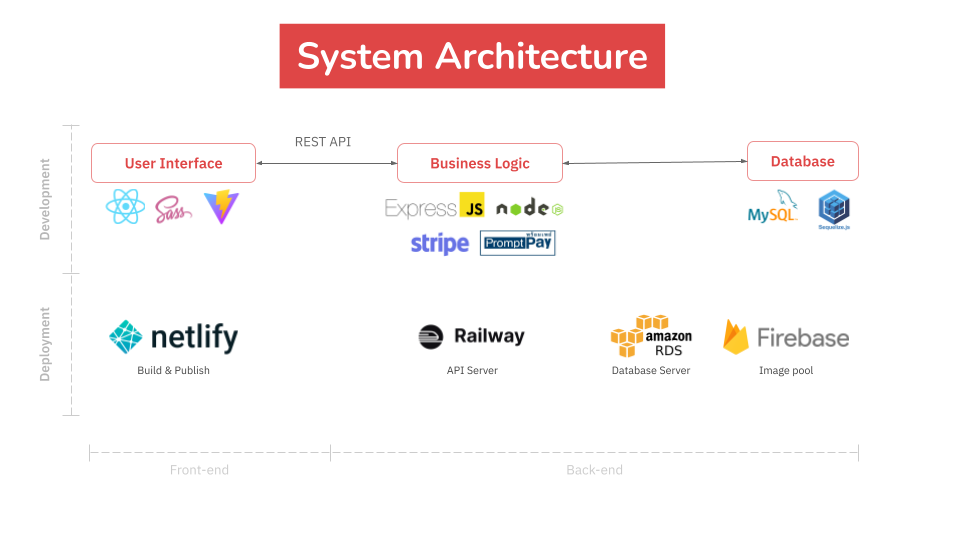
\includegraphics[width=\linewidth]{./image/System_Architecture.png}
    \end{center}
    \caption[System Architecture]{ภาพแสดงสถาปัตยกรรมระบบ}
    \label{fig:System_Architecture}
\end{figure}

\subsubsection{REST API}
แพลตฟอร์มของเราได้พัฒนาในรูปแบบของ MVC หรือ Model-View-Controller โดย Model คือ Database, Controller คือส่วนของ business logic หรือ server และสุดท้ายคือ View หรือ user interface อันเป็นส่วนที่ติดต่อกับผู้ใช้งาน

โดยการเชื่อมต่อระหว่างส่วนของ controller และส่วนของ view นั้น ได้เชื่อมต่อกันด้วย REST API กล่าวคือ หากจะต้องกระทำ business logic ใด ๆ หรือการ manipulate ใด ๆ กับ database ต้องกระทำด้วยการเรียกใช้งาน API endpoint ผ่าน HTTP methods เท่านั้น เช่น GET/POST/PUT/DELETE

ซึ่งประโยชน์ของการพัฒนาด้วย REST API คือการที่เราสามารถแยกส่วนของ user interface และ business logic ออกจากกันได้อย่างสิ้นเชิง โดยจุดนี้ได้อำนวยความสะดวกทีมผู้พัฒนาในการพัฒนาแต่ละส่วนโดยไม่จำเป็นต้องรอให้ส่วนใดส่วนหนึ่งพัฒนาเสร็จสิ้นก่อนจึงจะดำเนินการต่อได้ \\ \\
\begin{figure}[!ht]
    \begin{center}
    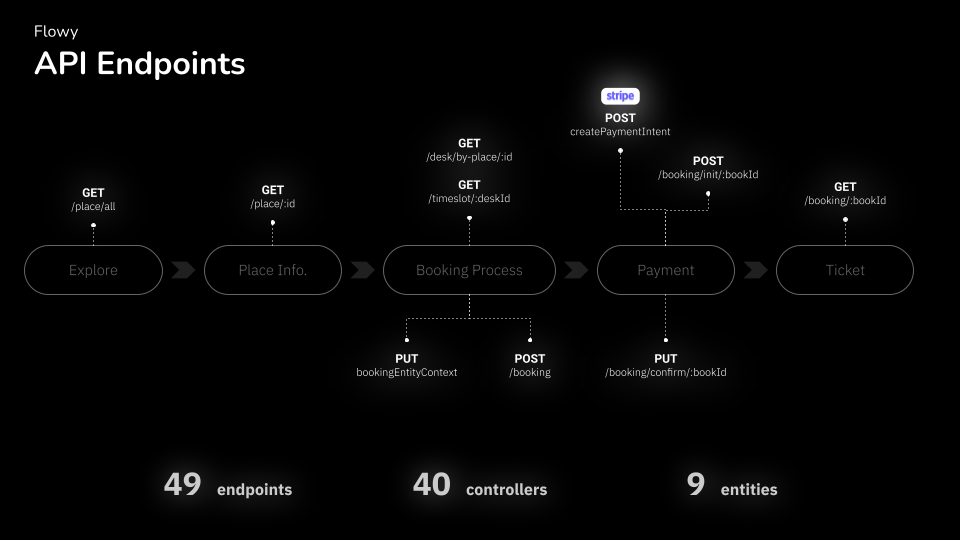
\includegraphics[width=\linewidth]{./image/API_Endpoints.png}
    \end{center}
    \caption[API Endpoints]{ภาพแสดงตัวอย่างของ API endpoint บางส่วนที่ได้ใช้งานบทแอปพลิเคชัน Flowy}
    \label{fig:API_Endpoints}
\end{figure}

\subsection{Database Design \& Schema}
ฐานข้อมูลที่เลือกใช้เป็นฐานข้อมูลประเภท SQL โดยมีองค์ประกอบดังรูปที่~\ref{fig:Database_schema_1} และมีรายละเอียดของข้อมูลดังต่อไปนี้ โดยเรียงลำดับตามแนวคิด parent entity ไปยัง children entity

\subsubsection{User}
เป็น entity ที่ใช้เก็บข้อมูลประจำตัวทั่วไปของผู้ใช้งานฝั่ง Flowy เพื่อใช้ระบุตัวตน (เมื่อทางราชการขอความร่วมมือ) และการเพื่ออำนวยความปลอดภัยให้กลับผู้ให้เช่าหรือ Flowider เมื่อเกิดเหตุการณ์ไม่พึงประสงค์ขึ้น ประกอบไปด้วย

\subsubsection{Flowider}
เป็น entity ที่ใช้เก็บข้อมูลประจำตัวทั่วไปของผู้ใช้งานฝั่ง Flowy เพื่อใช้ระบุตัวตน (เมื่อทางราชการขอความร่วมมือ), เพื่อทำการโอนเงินค่าใช้บริการจาก User และการเพื่ออำนวยความปลอดภัยให้กลับผู้เช่าหรือ Flowy เมื่อเกิดเหตุการณ์ไม่พึงประสงค์ขึ้น

\subsubsection{Place}
เป็น entity ที่ใช้เก็บข้อมูลรายละเอียดของสถานที่ที่ Flowider เป็นเจ้าของ เช่น ชื่อสถานที่, พิกัดของสถานที่, ที่อยู่เป็นลายลักษณ์อักษร, เวลาเปิด-ปิด เป็นต้น

\subsubsection{Amenity และ Specification}
เป็น 2 entities ที่ใช้เก็บรายละเอียดเพิ่มเติมของสถานที่นั้น ๆ ว่ามีลักษณะเป็นอย่างไร, เหมาะกับการใช้งานแบบไหนและมีสิ่งอำนวยความสะดวกใดให้บริการบ้าง เพื่อให้ user ใช้ประกอบการตัดสินใจได้ดียิ่งขึ้น

\subsubsection{Desk}
เป็น entity ที่ใช้เก็บข้อมูลจำเพาะของโซนโตะที่ให้บริการ โดยแนวคิดคือพื้นที่ของร้านต่าง ๆ จะถูกแบ่งออกเป็นโซนให้บริการ และเราจะเรียกแต่ละโซนเหล่านั้นว่า Desk ซึ่งแต่ละ Desk ใน entity นี้นั้นไม่จำเป็นต้องมีแค่โต๊ะเดียวตามชื่อของ entity ก็ได้

ซึ่ง attribute ในนี้จะเก็บค่าที่จำเป็นต่อการจองต่าง ๆ เช่น ที่นั่งต่ำสุดที่เข้าใช้งานได้รวมถึงจำนวนคนสูงสุดที่จะเข้าใช้งานได้, ประเภทของโต๊ะว่าเป็น Hot Desk รึเปล่า เป็นต้น (Hot Desk คือรูปแบบการจัดพื้นที่สำนักงานโต๊ะส่วนกลาง ที่เน้นตอบโจทย์เรื่องของ Open Space และความยืดหยุ่นในการทำงานและอิสระของพนักงานมากยิ่งขึ้นโดยให้พนักงานในองค์กรสามารถมาใช้โต๊ะทำงานส่วนกลางในเวลาใดก็ได้ ตำแหน่งไหนก็ได้)

\subsubsection{Timeslot}
เป็น entity ที่ใช้เก็บ time slot ทั้งหมดที่ถูก generate โดยอัตโนมัติจากเวลาที่ตั้งไว้บน server และค่าที่เปลี่ยนแปลงได้มีเพียงแค่ status และ occupied\_seat ที่บ่งบอกสถานะการใช้งานและจำนวนคนที่เข้าใช้งานตามลำดับ

\subsubsection{Booking}
เป็น entity ที่ใช้เก็บรายละเอียดสำคัญที่เกี่ยวข้องการจองทั้งหมดรวมถึงรายละเอียดและสถานะของการชำระค่าบริการด้วยเช่นกัน

\begin{landscape}
    \begin{figure}[ht]
        \begin{center}
            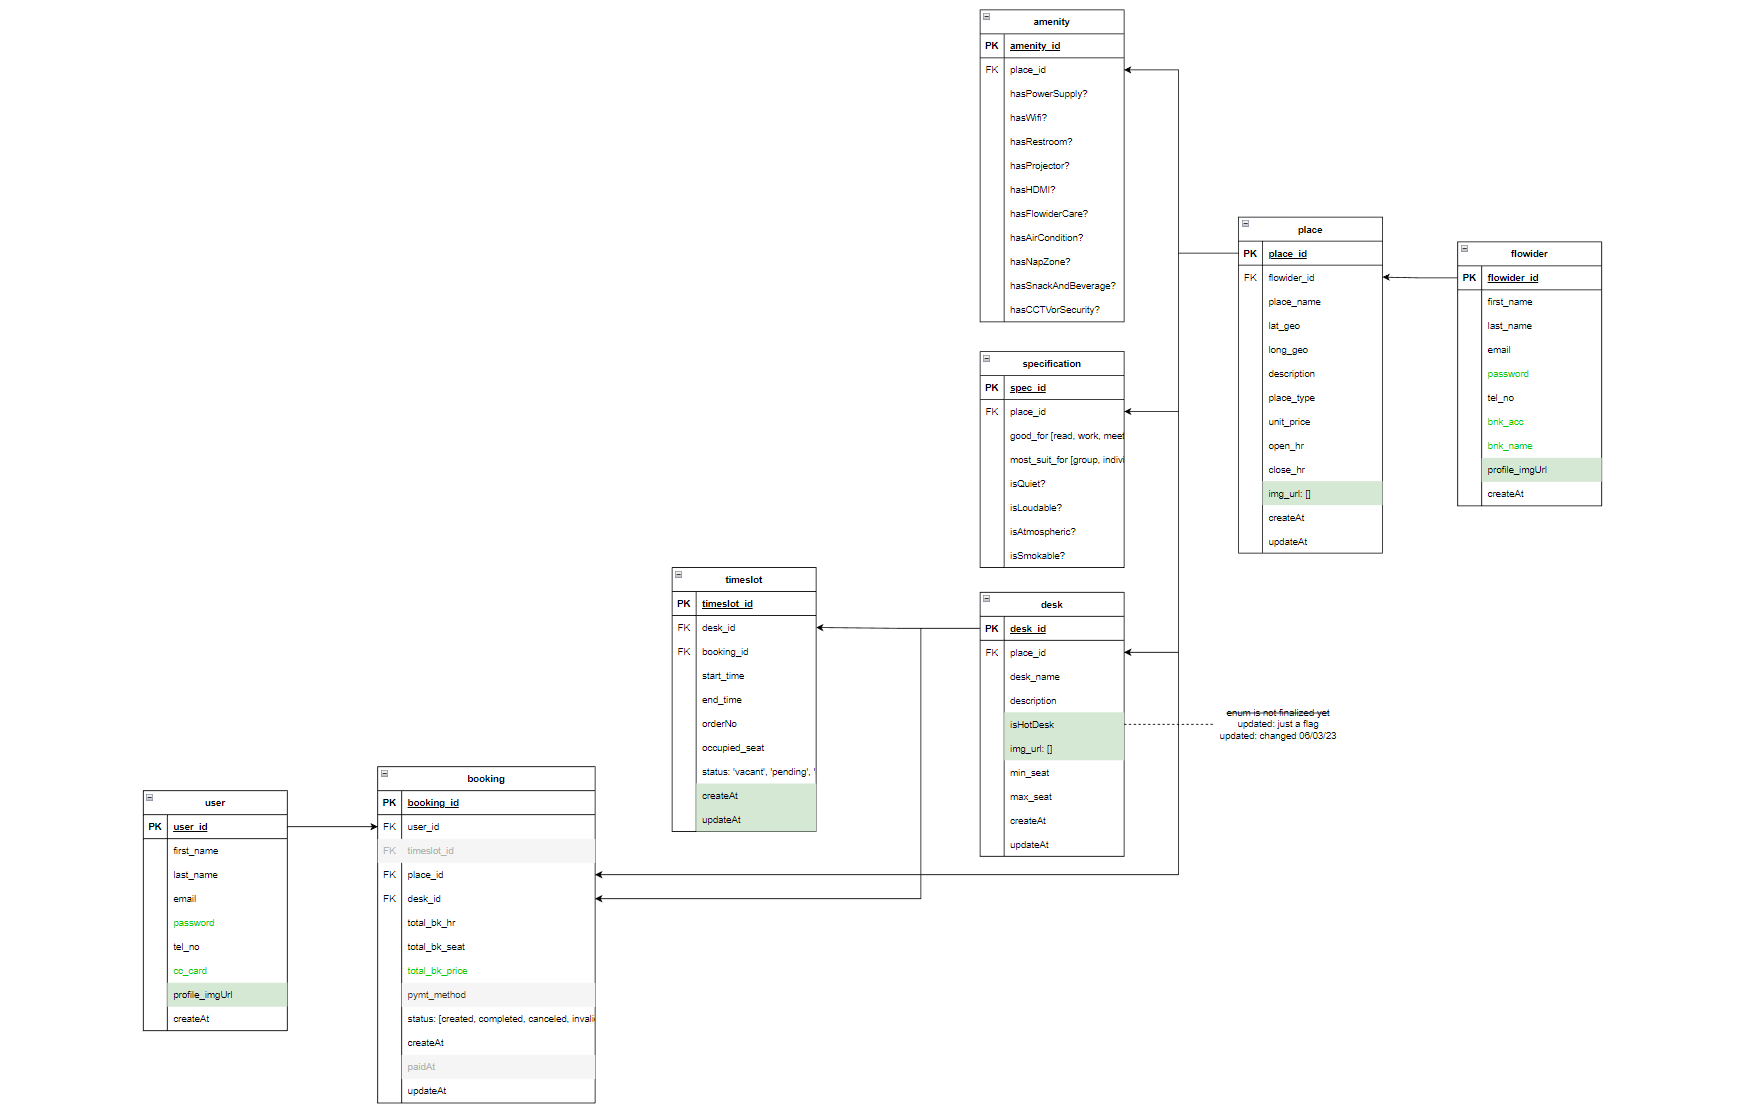
\includegraphics[width=8.1in]{./image/Database_schema_1.png}
        \end{center}
        \caption[Database Schema]{แผนภาพแสดงโครงสร้างของฐานข้อมูล}
        \label{fig:Database_schema_1}
    \end{figure}
\end{landscape}

\subsection{Time Slot Design}
\subsubsection{Generation Logic}
การออกแบบการทำงานของการเลือกช่วงเวลาใช้บริการที่แยกตามแต่ละ Desk นั้นถือเป็นหนึ่งในความท้าทายของโครงงานนี้ เนื่องจากมีแนวคิดหลากหลายรูปแบบที่เราสามารถนำมาปรับใช้ได้ โดยเบื้องต้นเราได้นึกถึงการจองตั๋วเพื่อเข้าชมภาพยนตร์ แต่แนวคิดนี้ก็ตกไปเนื่องจากติดปัญหาในส่วนของผังที่นั่งที่จัดวางไม่เหมือนกันในแต่ละร้าน ซึ่งแตกต่างกับโรงภาพยนตร์ที่มีผังที่นั่งชัดเจนอย่างสิ้นเชิง

ในแนวความคิดต่อมาคือเพิ่มความ abstract มากขึ้นด้วยการเปลี่ยนเป็นแสดงผลแค่ช่วงเวลาอย่างเดียว แล้วให้ผู้ใช้งานกดเลือกช่วงเวลาที่ต้องการใช้งานเท่านั้น แต่เริ่มต้นเราต้องการให้ฝั่งของ user interface เป็นฝ่าย generate time slot ทั้งหมดตามเงื่อนไขเวลาเปิด-ปิดทำการของสถานที่นั้น เมื่อผู้ใช้งานเลือกก็ส่งรายละเอียดต่าง ๆ เข้ามายัง entity Timeslot ก็เป็นอันเสร็จสิ้น แต่แนวคิดนี้ก็ตกไปเช่นกันเนื่องจากการทำงานที่หนักเกินไปของฝั่ง user interface และติดปัญหาเรื่อง reference เวลาทำ payment process

สุดท้ายเราจึงเลือกวิธีการ generate time slot ทั้งหมดโดยอัตโนมัติผ่านการทำงานของ business logic โดยมีหลักการคิดคือคำนวณหาผลต่างของเวลาเปิด-ปิด (usable window) ของแต่ละสถานที่ แล้วนำไปสร้าง time slot ใหม่ให้แต่ละโต๊ะ ในทุก ๆ โต๊ะ, ทุก ๆ ร้าน และทุก ๆ วัน

\begin{equation}
    amt.\;of\;timeslot = places\;amt.\;entire\;DB\times desks\;amt.\;entire\;DB \times usable\;window
\end{equation}

ตัวอย่างเช่น หากแพลตฟอร์มของเรามีทั้งหมด 10 สถานที่ แต่ละที่มี usable window จากการคำนวณเวลาเปิด-ปิด 10 ชั่วโมงเหมือนกันทุกร้าน และแต่ละสถานที่มีทั้งหมด 10 โต๊ะเหมือนกันหมด ก็จะคำนวณได้ว่า

\begin{equation}
    amt.\;of\;timeslot = 10 \times 10 \times 10
\end{equation}

ในวันต่อ ๆ ไปหากไม่มีจำนวนร้านหรือโต๊ะเพิ่มขึ้นเลย แต่ละวันจะมี time slot ถูก generate ขึ้นวันละ 1000 time slots ซึ่งเราได้ทำการเขียนคำสั่งที่คอยลบ time slot ที่มีสถานะ *vacant* ไว้แล้วในทุก ๆ สัปดาห์ เพื่อลดปัญหาการใช้พื้นที่ฐานข้อมูลเกินจำเป็น

ซึ่งจากวิธีการนี้ทำให้เราลดภาระการทำงานของ user interface ได้ รวมถึงลดความยุ่งยากของทีมผู้พัฒนาด้วยเช่นกัน

\subsubsection{Component Design}
เมื่อเราได้วิธีการในการสร้าง time slot แล้ว ในส่วนต่อไปคือการออกแบบการทำงานของ user interface ที่จะทำให้การปรับเปลี่ยนรายละเอียดของ time slot มีประสิทธิภาพที่สุด เราจะได้ใช้หลักแนวคิดแบบ immutable component กล่าวคือเราจะไม่ทำการปรับเปลี่ยนค่าใด ๆ ของ time slot ทั้งสิ้น และยกหน้าที่การเปลี่ยนแปลงค่าต่าง ๆ ให้กับ business logic เท่านั้น

เพราะฉะนั้นสิ่งที่เราทำคือการสร้าง array ออกมา 1 arrays คือ chosenTimeSlot ที่เป็น array ของ time slot ที่ถูกกดเลือกเอาไว้ เพื่อเก็บ object ของ time slot เอาไว้ เตรียมส่งกลับไปให้ business logic ดำเนินการต่อ

เมื่อผู้ใช้งานทำการกดเลือก เราจะทำการ push object ของ time slot นั้น เข้าสู่ chosenTimeSlot และทำการ pop ออกจาก chosenTimeSlot เมื่อมีการกดอีกครั้งหนึ่ง (เป็นการยกเลิกการเลือก) ในขณะเดียวกันกับที่เกิด action เหล่านี้ ก็ต้องทำการเปลี่ยน styling ที่แสดงผล time slot ที่ถูกเลือกด้วยการใช้งาน state ของ React TS ด้วยเช่นกัน เมื่อสิ้นสุดการเลือกแล้ว ค่าใน chosenTimeSlot คือสิ่งที่เราจะใช้ต่อไปในส่วนของ business logic

\subsection{Payment Process}
ระบบชำระค่าบริการเป็นส่วนที่ท้าทายที่สุดในโครงงานนี้ เนื่องจากเป็นส่วนที่ละเอียดอ่อนและต้องทำงานกับ credential ของผู้ใช้งาน หากเกิดปัญหาจากการใช้งานอาจทำให้เกิดการฟ้องร้องเอาผิดขึ้นมาได้ ทางทีมผู้พัฒนาจึงใช้บริการของ Stripe ซึ่งเป็น payment gateway provider ที่ผู้ประกอบการหรือนักพัฒนาซอฟต์แวร์ทั่วโลกเลือกใช้งาน ตัวอย่างประโยชน์ของการใช้งาน Stripe เช่น
\begin{itemize}
    \item มีตัวเลือกการชำระเงินครอบครัวเกือบทุกรูปแบบในทุกประเทศทั่วโลก
    \item มี documentation ที่ดี ปฏิบัติตามได้อย่างไม่สับสน
    \item มี developer community ที่กว้างขวาง พร้อมช่วยเหลือเมื่อเกิดปัญหา เนื่องจาก Stripe ถูกใช้งานกว่า 1,000,000 เว็บไซต์ทั่วโลก
    \item implementation ง่าย ขั้นตอนไม่ยุ่งยาก
\end{itemize}
เนื่องจากทีมผู้พัฒนาไม่มีประสบการณ์การทำระบบชำระค่าบริการมาก่อน จึงต้องการทำความเข้าใจโดยละเอียดทั้งหมดถึงกระบวนการจองไปจนถึงการชำระค่าบริการ ว่าเราจะต้องทำการส่งผ่าน/เปลี่ยนค่าของรายละเอียดการจองอย่างไร และจะติดต่อกับ Stripe API, Flowy API ได้อย่างไร

เราจึงทำการวาด service blueprint ดังรูปที่~\ref{fig:service_blueprint} เพื่อทำให้ทีมผู้พัฒนาเห็นภาพร่วมกันว่า ลักษณะโครงสร้างการทำงานจะมีลักษณะเช่นไร และทำให้ผู้พัฒนาสามารถปรับปรุงการส่งผ่านรายละเอียดการจองเป็นไปได้อย่างมีประสิทธิภาพมากยิ่งขึ้น

\subsection{UX/UI Design}
\subsubsection{Flowy}
\begin{itemize}
    \item Login: หน้าเข้าสู่ระบบสําหรับผู้ใช้งาน (รูปที่~\ref{fig:Flowy_login})
    \item Register: หน้าสมัครสมาชิกสําหรับผู้ใช้งาน (รูปที่~\ref{fig:Flowy_register})
    \item Explore: หน้าแสดงสเปซที่ให้บริการบนแพลตฟอร์ม Flowy (รูปที่~\ref{fig:Flowy_explore})
    \item Place information: หน้าแสดงรายระเอียดของสเปซ (รูปที่~\ref{fig:Flowy_info_1} และ~\ref{fig:Flowy_info_2})
    \item Booking
    \begin{itemize}
        \item Booking customer amount: หน้าระบุจํานวนผู้เข้าใช้บริการ (รูปที่~\ref{fig:Flowy_book_ctm_amt})
        \item Booking desk: หน้าเลือกโต๊ะสําหรับทํากิจกรรมต่าง ๆ (รูปที่~\ref{fig:Flowy_book_desk})
        \item Booking time slot: หน้าระบุเวลาเข้าใช้บริการ (รูปที่~\ref{fig:Flowy_book_time_slot})
    \end{itemize}
    \item Payment: หน้าชําระค่าบริการ (รูปที่~\ref{fig:Flowy_payment})
    \item Ticket: หน้าแสดงรายระเอียดตั๋ว (รูปที่~\ref{fig:Flowy_ticket_1} และ~\ref{fig:Flowy_ticket_2})
    \item Account: หน้าแสดงบัญชีผู้ใช้ (รูปที่~\ref{fig:Flowy_account})
    \item Booking history: หน้าแสดงประวิติการจองสเปซ (รูปที่~\ref{fig:Flowy_book_history})
\end{itemize}

\subsubsection{Flowider}
\begin{itemize}
    \item Login: หน้าเข้าสู่ระบบสําหรับผู้ใช้งาน (รูปที่~\ref{fig:Flowider_login})
    \item Register: หน้าสมัครสมาชิกสําหรับผู้ใช้งาน (รูปที่~\ref{fig:Flowider_register})
    \item Booking management: หน้าจัดการรายการจอง (รูปที่~\ref{fig:Flowider_booking_mgmt})
    \item Schedule: หน้าแสดงรายระเอียดการจองของแต่ละสเปซ (รูปที่~\ref{fig:Flowider_schedule})
    \item Account: หน้าแสดงบัญชีผู้ใช้ของผู้ใช้บริการ (รูปที่~\ref{fig:Flowider_account})
    \item Edit account: หน้าแก้ไขข้อมูลส่วนตัวของผู้ให้บริการ (รูปที่~\ref{fig:Flowider_edit_account})
    \item Space management: หน้าจัดการสเปซ (รูปที่~\ref{fig:Flowider_space_mgmt})
    \item Edit Space: หน้าแก้ไขข้อมูลของสเปซ (รูปที่~\ref{fig:Flowider_space_edit_1} และ~\ref{fig:Flowider_space_edit_2})
    \item Create place
    \begin{itemize}
        \item Onboarding: หน้าเตรียมข้อมูลของสเปซก่อนทําการลงทะเบียน (รูปที่~\ref{fig:Flowider_onboarding_1}) และหน้าเตรียมข้อมูลของโต๊ะก่อนทําการลงทะเบียน (รูปที่~\ref{fig:Flowider_onboarding_2})
        \item Place category: หน้าระบุประเภทของสเปซ (รูปที่~\ref{fig:Flowider_place_category})
        \item Place information: หน้าระบุรายละเอียดของสเปซ (รูปที่~\ref{fig:Flowider_place_info_1} และ~\ref{fig:Flowider_place_info_2})
        \item Specification: หน้าระบุความเฉาะเจาะจง (รูปที่~\ref{fig:Flowider_place_Specification})
        \item Amenity: หน้าระบุสิ่งอํานวยความสะดวก (รูปที่~\ref{fig:Flowider_place_amenity})
        \item Place image upload: หน้าเพิ่มรูปภาพของสเปซ (รูปที่~\ref{fig:Flowider_place_img})
        \item Place location: หน้าระบุตําแหน่งของสเปซ (รูปที่~\ref{fig:Flowider_place_location})
        \item Desk: หน้าระบุรายระเอียดของโต๊ะ (รูปที่~\ref{fig:Flowider_desk_1} และ~\ref{fig:Flowider_desk_2})
    \end{itemize}
\end{itemize}

\section{ขั้นตอนการดำเนินงาน}
\subsection{ทำความเข้าใจปัญหา}
เนื่องจากพวกเราเป็นนักศึกษามหาวิทยาลัย ทุกช่วงที่การสอบกลางภาคหรือปลายภาคใกล้เข้ามา เรามันจะปัญหาในเรื่องของการไม่มีพื้นที่ที่เพียงพอสำหรับทำกิจกรรมต่าง ๆ เช่น การอ่านหนังสือ, ทำงานกลุ่มหรือประชุม เป็นต้น ทำให้เราเริ่มมีความคิดว่า ``ปัญหานี้มักจะเกิดมาจากปริมาณการใช้งานในเวลาที่ใกล้เคียงกันโดยอุปทานหรือพื้นที่ที่ให้ใช้สอยมีไม่เพียงพอต่อความต้องการ''

เมื่อเราพบเจอกับปัญหาเช่นนี้แล้ว เราจึงคิดต่อไปว่าอยากที่จะแก้ไขปัญหานี้ แต่ก่อนที่จะเริ่มขั้นตอนการพัฒนาผลิตภัณฑ์หรือ solution ใดที่จะเข้ามาแก้ปัญหา เราต้องการแน่ใจก่อนว่าปัญหาที่เราเจอไม่ได้มีเพียงเราเจอแค่กลุ่มเดียวหรือแค่กลุ่มเล็ก ๆ เท่านั้น เราจึงทำการออกแบบสำรวจเพื่อทำการสำรวจปัญหาและทำความเข้าใจปัญหาเพิ่มเติมในเชิงลึกขึ้นถึงความต้องการที่แท้จริงของผู้ประสบปัญหาที่คล้ายคลึงกับเรา

โดยทั้งหมดที่กล่าวมานี้ คือขั้นตอนแรกของกระบวนการ Design Thinking นั่นคือ ``การทำความเข้าอกเข้าใจ (Empathize)''

\subsection{กำหนดปัญหาและทำแบบสำรวจ}
ในการทำแบบสำรวจได้ถูกแบ่งออกเป็น 3 ส่วนด้วยกัน ดังนี้
\begin{enumerate}
    \item คำถามทั่วไป (General Question)
    \begin{itemize}
        \item เพศ
        \item อายุ
        \item อาชีพ
        \item รับดับการศึกษาสูงสุด
        \item ชื่อสถานศึกษา
        \item คณะที่กำลังศึกษา
        \item รายได้เฉลี่ยในแต่ละเดือน
    \end{itemize}
    \item คำถามเชิงพฤติกรรม (Behavioral Question)
    \begin{itemize}
        \item โดยลักษณะนิสัยของท่านแล้ว ท่านชอบอ่านหนังสือ / ทำงานคนเดียวหรือเป็นกลุ่ม
        \item โดยปกติแล้วคุณอ่านหนังสือเพื่อเตรียมตัวสอบที่ใด
        \item โดยปกติแล้วคุณทำงานกลุ่ม / ทำงานบริษัทที่ใด
        \item ความสะดวกจากการใช้งานสถานที่เหล่านั้น
        \item ท่านมักเจอปัญหาอะไรจากสถานที่ที่คุณใช้บริการอ่านหนังสือ / ทำงานบ้าง
        \item โดยปกติแล้วท่านแก้ไขปัญหาเหล่านั้นอย่างไร
    \end{itemize}
    \item คำถามเพื่อหาวิธีการแก้ไขปัญหา (Solution Finding)
    \begin{itemize}
        \item หากมีตัวช่วยที่สามารถแก้ไขปัญหาการหาที่อ่านหนังสือ / ทำงานดังที่ท่านได้ระบุก่อนหน้านี้ได้ ท่านมีความสนใจมาก-น้อยเท่าใด
        \item ตัวช่วยดังกล่าวจะมีลักษณะคล้ายคลึงกับ Airbnb สำหรับการหาที่อ่านหนังสือ / ทำงาน (คือมีลักษณะเป็นการเช่าพื้นที่ของเจ้าของที่พักเป็นรายชั่วโมง แทนที่จะเป็นการเช่าที่พักรายคืนเหมือน Airbnb) ท่านมีความสนใจที่จะใช้งานมากเพียงใด
        \item ความเร่งด่วนที่ต้องการตัวช่วยนี้เข้ามาทำให้ชีวิตคุณสะดวกมากขึ้น มีมาก-น้อยเพียงใด
        \item คุณต้องการใช้งานตัวช่วยนี้ผ่านอุปกรณ์ประเภทใดมากที่สุด
        \item คุณต้องการให้สถานที่อ่านหนังสือ / ทำงานนั้นๆ ต้องมีสิ่งอำนวยความสะดวกอะไรบ้าง
        \item ราคาในใจสูงสุดที่จะยอมจ่ายเพื่อเช่าสถานที่นั้น จะมีราคาเท่าใดต่อ 1 ชั่วโมง
        \item ท่านมีแนวโน้มจะใช้ตัวช่วยนี้กับเพื่อนของคุณมากน้อยเพียงใด
        \item ท่านคาดหวังที่จะได้ประสบการณ์การใช้งาน (user experience) จากตัวช่วยนี้อย่างไรบ้าง
        \item คำแนะนำเพิ่มเติมถึงผู้พัฒนา
    \end{itemize}
\end{enumerate}

\subsection{ออกแบบ Proof of Concept}
เมื่อได้ผลสำรวจมาแล้ว เราจึงเริ่มออกแบบตัวต้นแบบของเราด้วยการวิเคราะห์ปัญหาและความต้องการของผู้ทำแบบสำรวจ เพื่อให้การใช้งานและประสบการณ์ใช้งานราบรื่นที่สุด
\begin{itemize}
    \item ออกแบบตัวต้นแบบ UX/UI ด้วย \href{https://www.figma.com/file/y0b4Wo3axU0TD5uoZHBhZM/Flowy?node-id=0-1&t=JYeTFmvNhNrmnj4b-0}{Figma}
    \item ออกแบบโครงสร้างแพลคฟอร์มและฐานข้อมูลด้วย \href{https://app.diagrams.net/#G1SVEf5xnuNXJhE77jdD0Rvaj5KxYkY-5y}{Draw.io}
\end{itemize}

\subsection{พัฒนาระบบ}
\begin{itemize}
    \item พัฒนาในส่วนของ user interface ตามที่ได้ทำการออกแบบ UX/UI
    \item พัฒนาในส่วนของ server ตามกระบวนการพื้นฐาน CRUD โดยใช้โปรแกรม Postman ในการทดสอบ API endpoint ต่าง ๆ
    \item พัฒนาโครงสร้างของ database ตาม schema ที่ได้ทำการออกแบบ โดยทดสอบหรือ query ตรวจสอบความถูกต้องของข้อมูลโดยไม่ผ่าน API endpoint ด้วย MySQL Workbench 8.0 CE ที่เชื่อมต่อโดยตรงกับ AWS RDS
\end{itemize}

\subsection{การทดสอบใช้งาน}
\begin{itemize}
    \item ทำการทดสอบระบบในแต่ละ function ในแต่ละหน้าทั้งแพลตฟอร์ม Flowy และ Flowider ว่าสามารถทำงานได้ถูกต้อง
    \item ทำการทดสอบการใช้งานในแต่ละ feature ของทั้งแพลตฟอร์ม Flowy และ Flowider ว่าการใช้งานราบรื่น ไม่มีส่วนใดผิดปกติ
    \item วางแผนการทดสอบการใช้งานแบบสาธารณะในเดือนมีนาคม 2566
\end{itemize}

% \begin{landscape}
%     \begin{figure}[ht]
%         \begin{center}
%             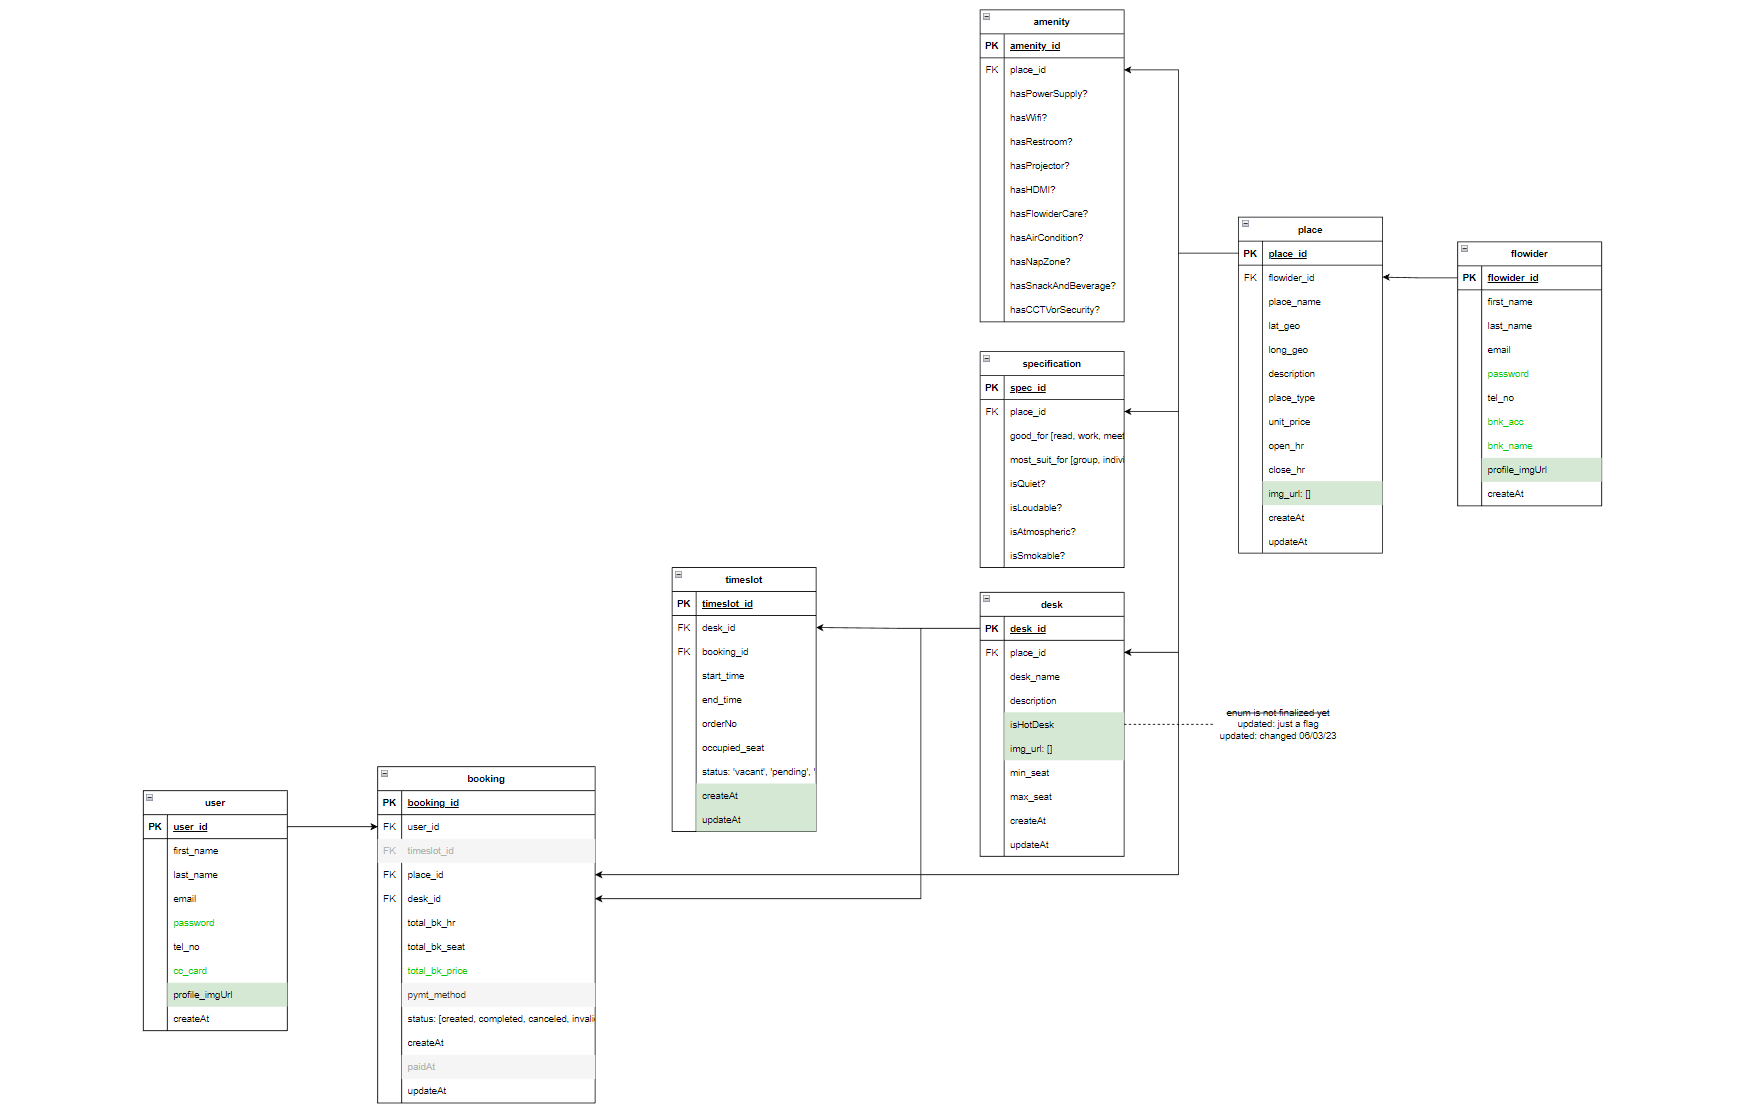
\includegraphics[width=8.1in]{./image/Database_schema_1.png}
%         \end{center}
%         \caption[Database Schema]{แผนภาพแสดงโครงสร้างของฐานข้อมูล}
%         \label{fig:Database_schema_1}
%     \end{figure}
% \end{landscape}
\begin{landscape}
    \begin{figure}[ht]
        \begin{center}
        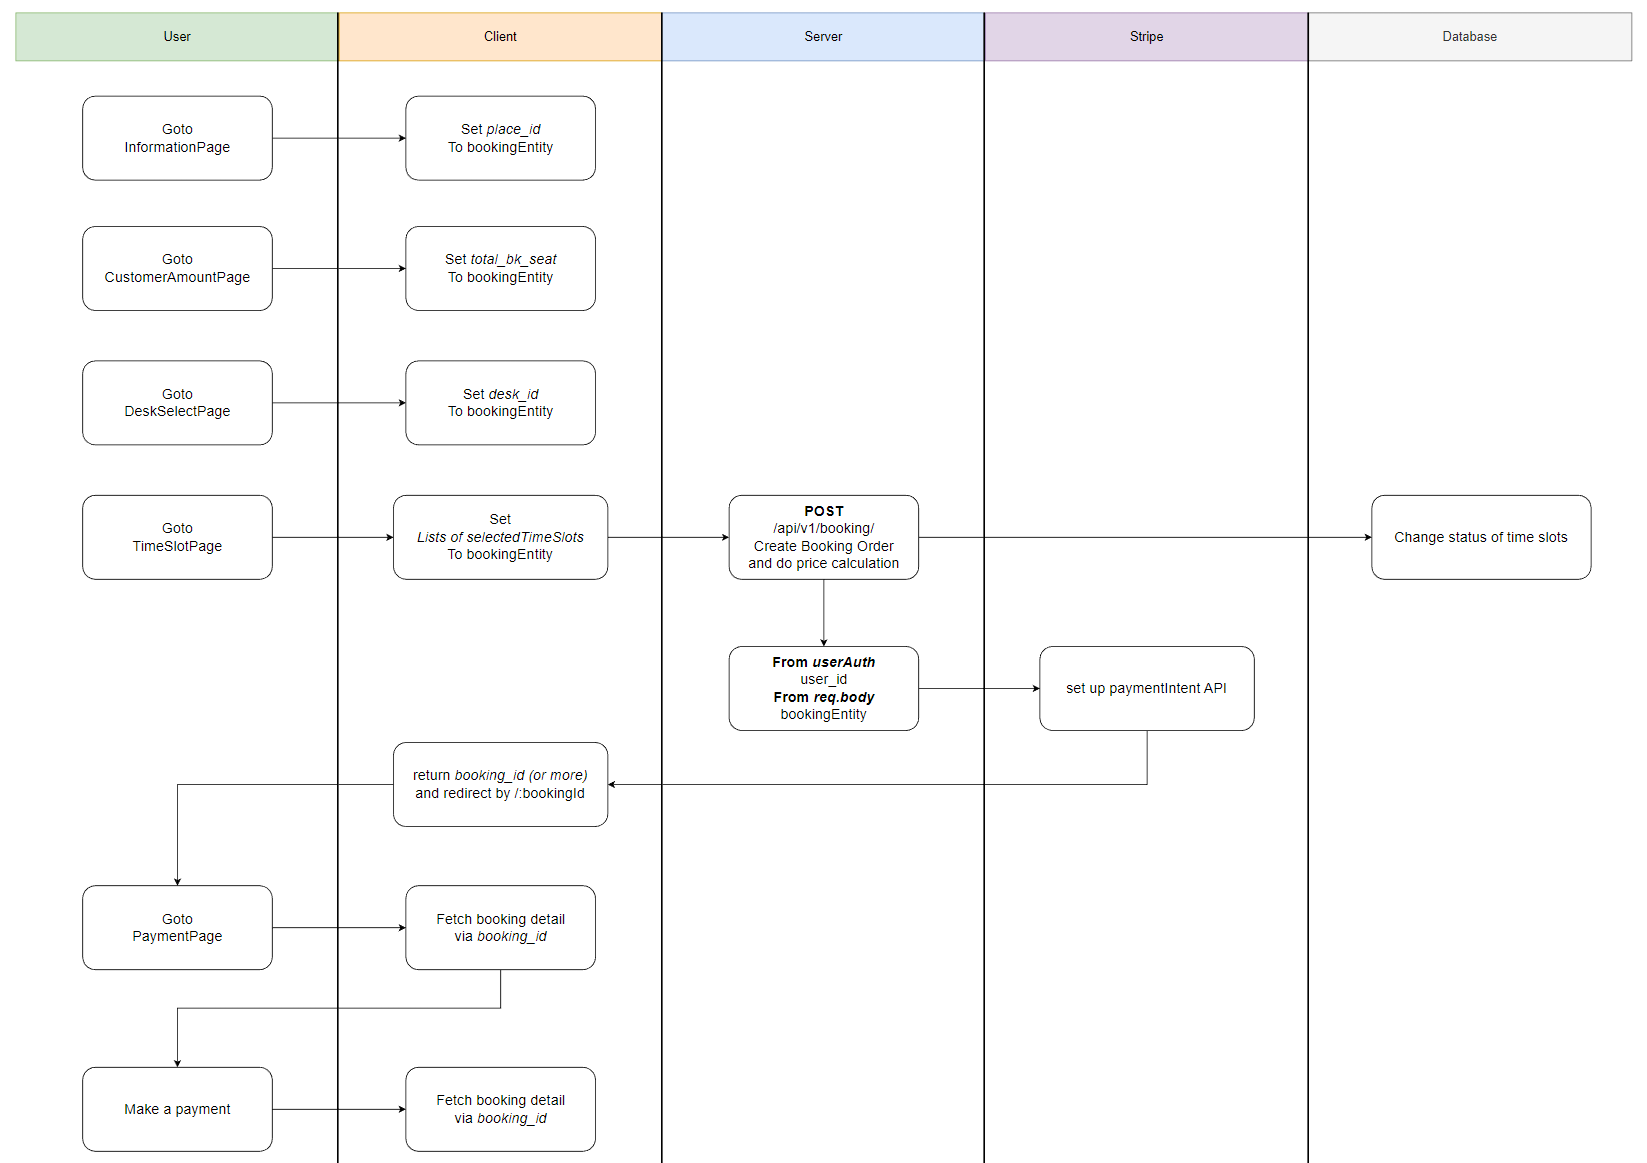
\includegraphics[width=7in]{./image/service_blueprint.png}
        \end{center}
        \caption[Payment service blueprint]{แผนผัง service blueprint การทำงานทั้งหมดของกระบวนการจองตั้งแต่เริ่มต้นจนถึงชำระค่าบริการ}
        \label{fig:service_blueprint}
    \end{figure}
\end{landscape}
\begin{figure}[t]
    \begin{center}
    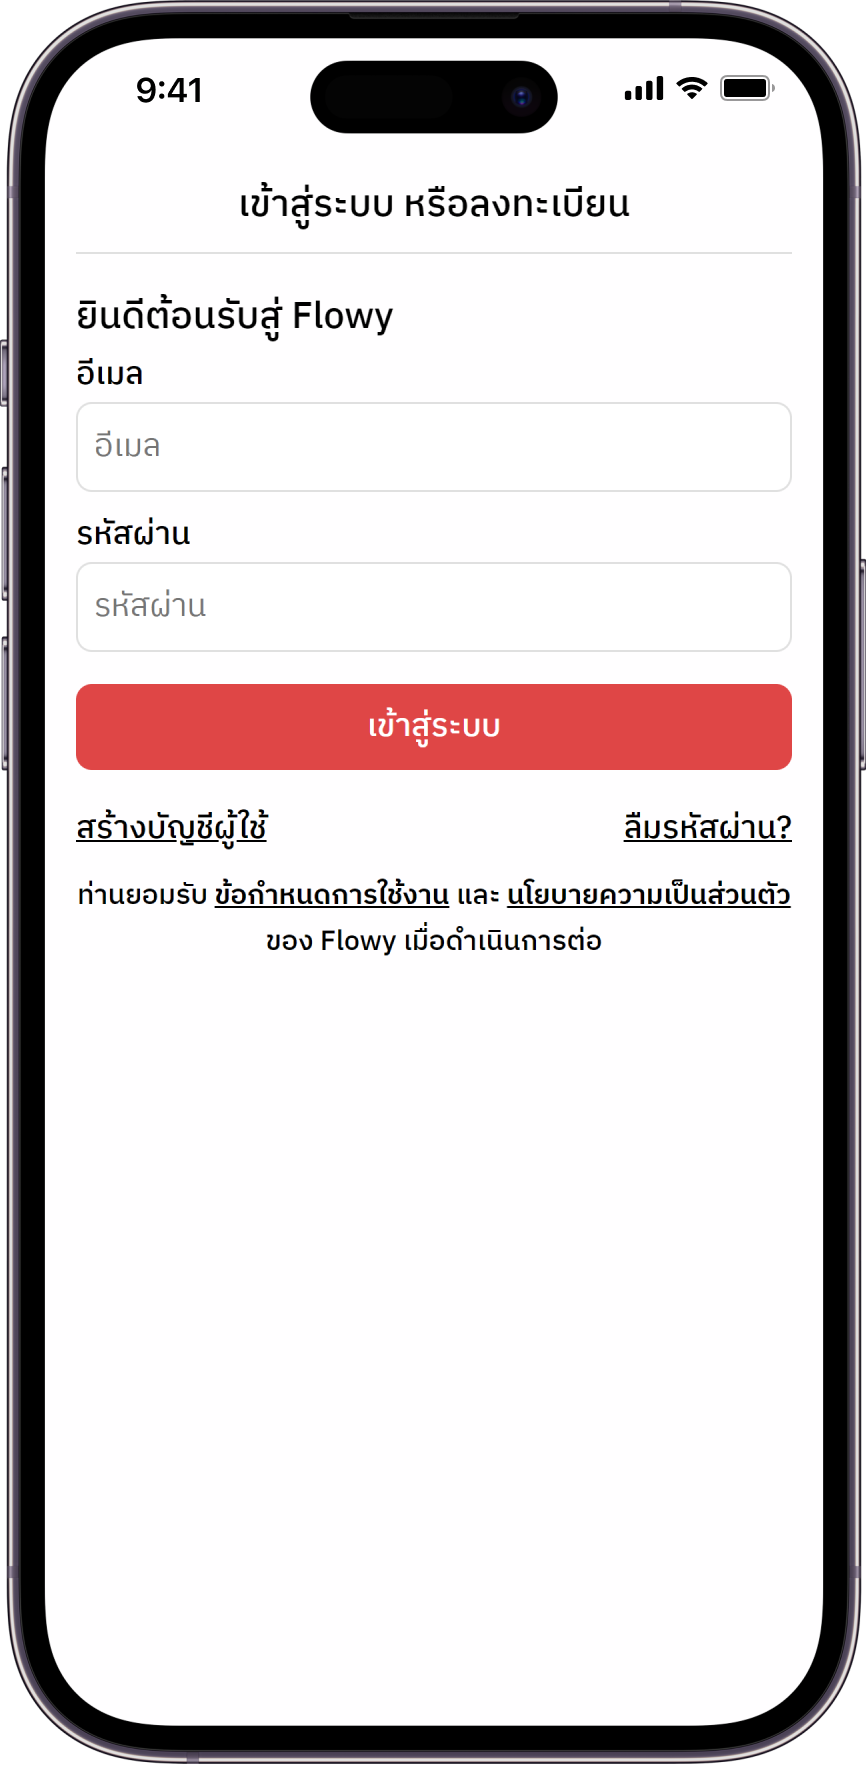
\includegraphics[width=1.9in]{./image/Flowy_login.png}
    \end{center}
    \caption[Flowy login]{หน้าเข้าสู่ระบบสำหรับผู้ใช้งาน (Flowy)}
    \label{fig:Flowy_login}
\end{figure}
\begin{figure}[ht]
    \begin{center}
    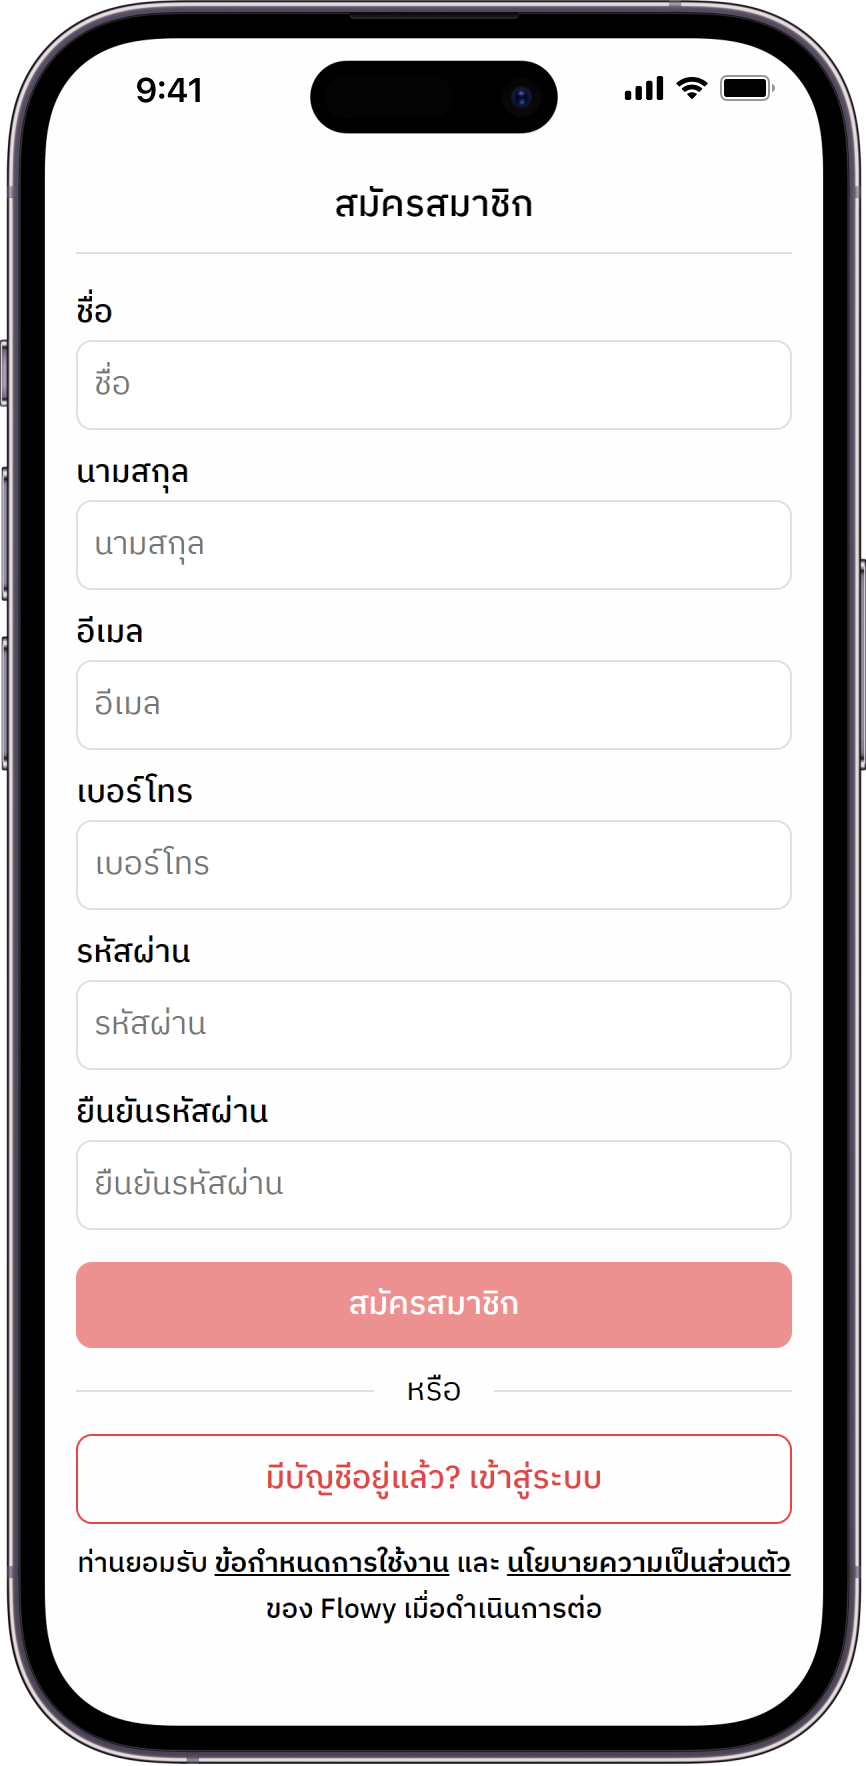
\includegraphics[width=1.9in]{./image/Flowy_register.png}
    \end{center}
    \caption[Flowy register]{หน้าสมัครสมาชิกสำหรับผู้ใช้งาน (Flowy)}
    \label{fig:Flowy_register}
\end{figure}
\begin{figure}[ht]
    \begin{center}
    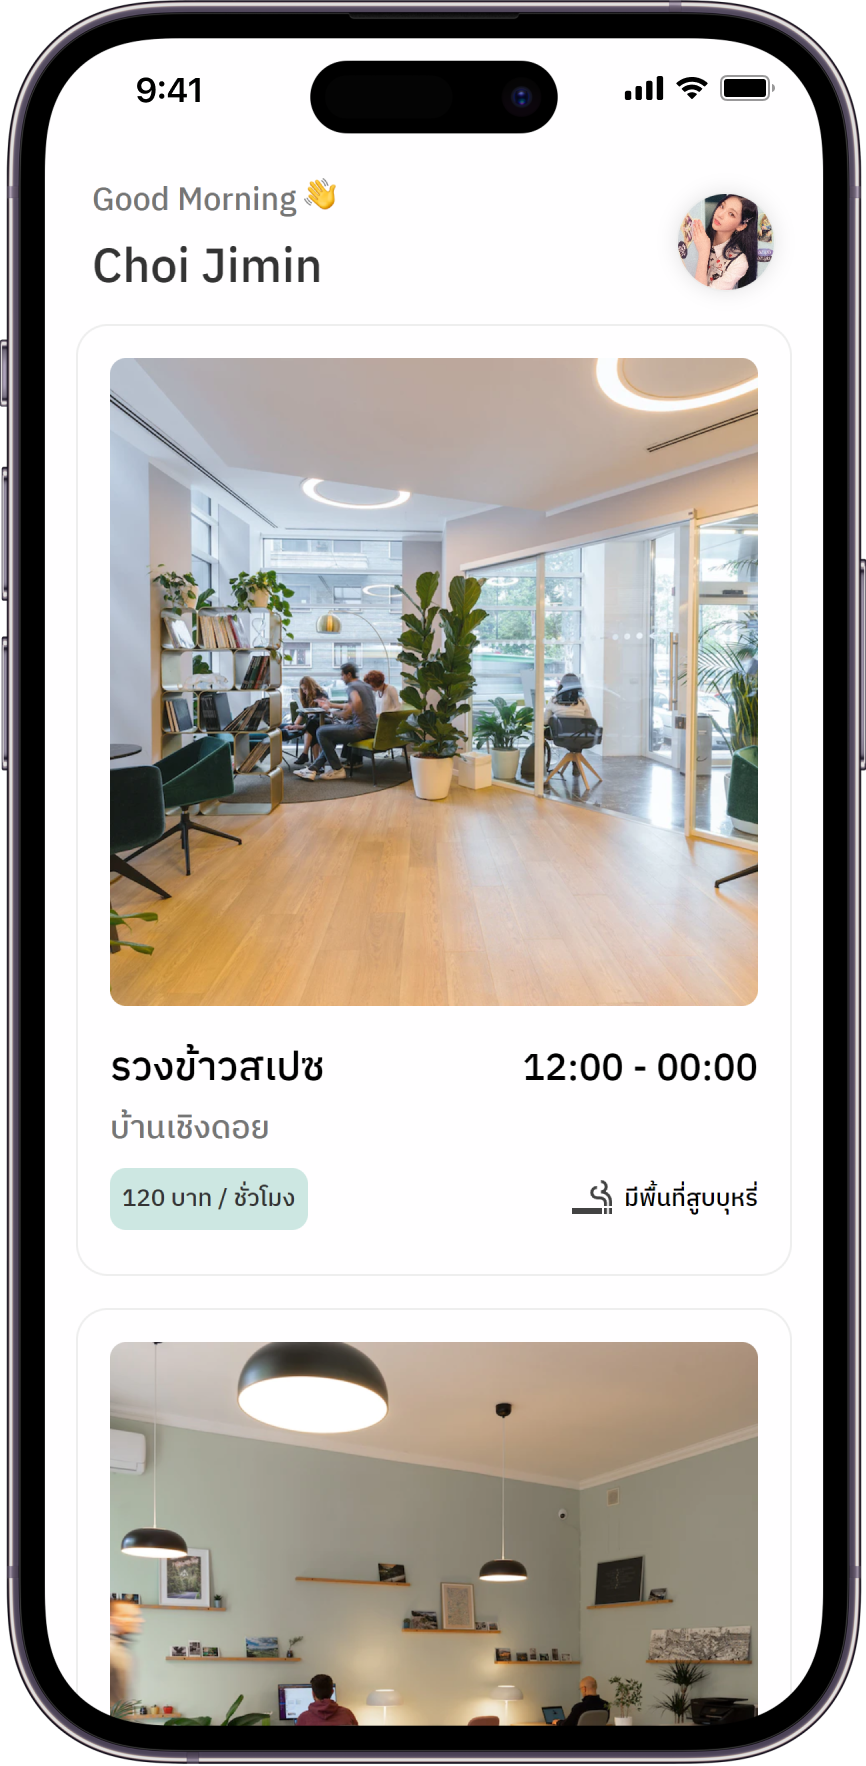
\includegraphics[width=1.9in]{./image/Flowy_explore.png}
    \end{center}
    \caption[Flowy explore]{หน้าแสดงสเปซที่ให้บริการบนแพลตฟอร์ม Flowy}
    \label{fig:Flowy_explore}
\end{figure}
\begin{figure}[ht]
    \begin{center}
    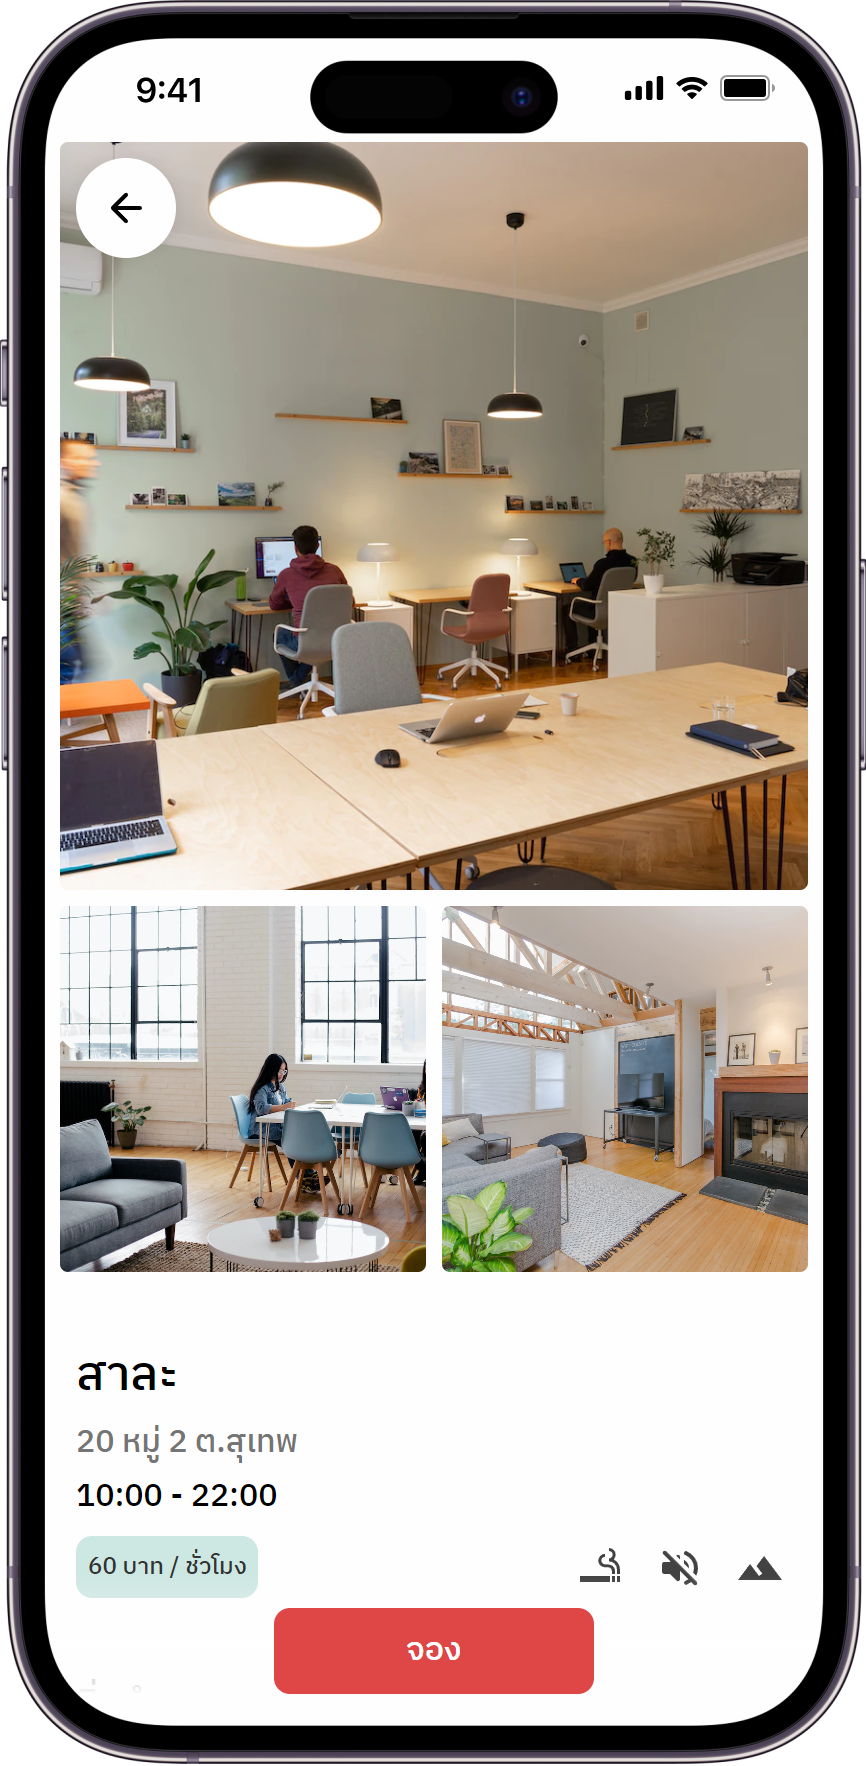
\includegraphics[width=1.9in]{./image/Flowy_info_1.png}
    \end{center}
    \caption[Flowy info 1]{หน้าแสดงรายระเอียดของสเปซ}
    \label{fig:Flowy_info_1}
\end{figure}
\begin{figure}[ht]
    \begin{center}
    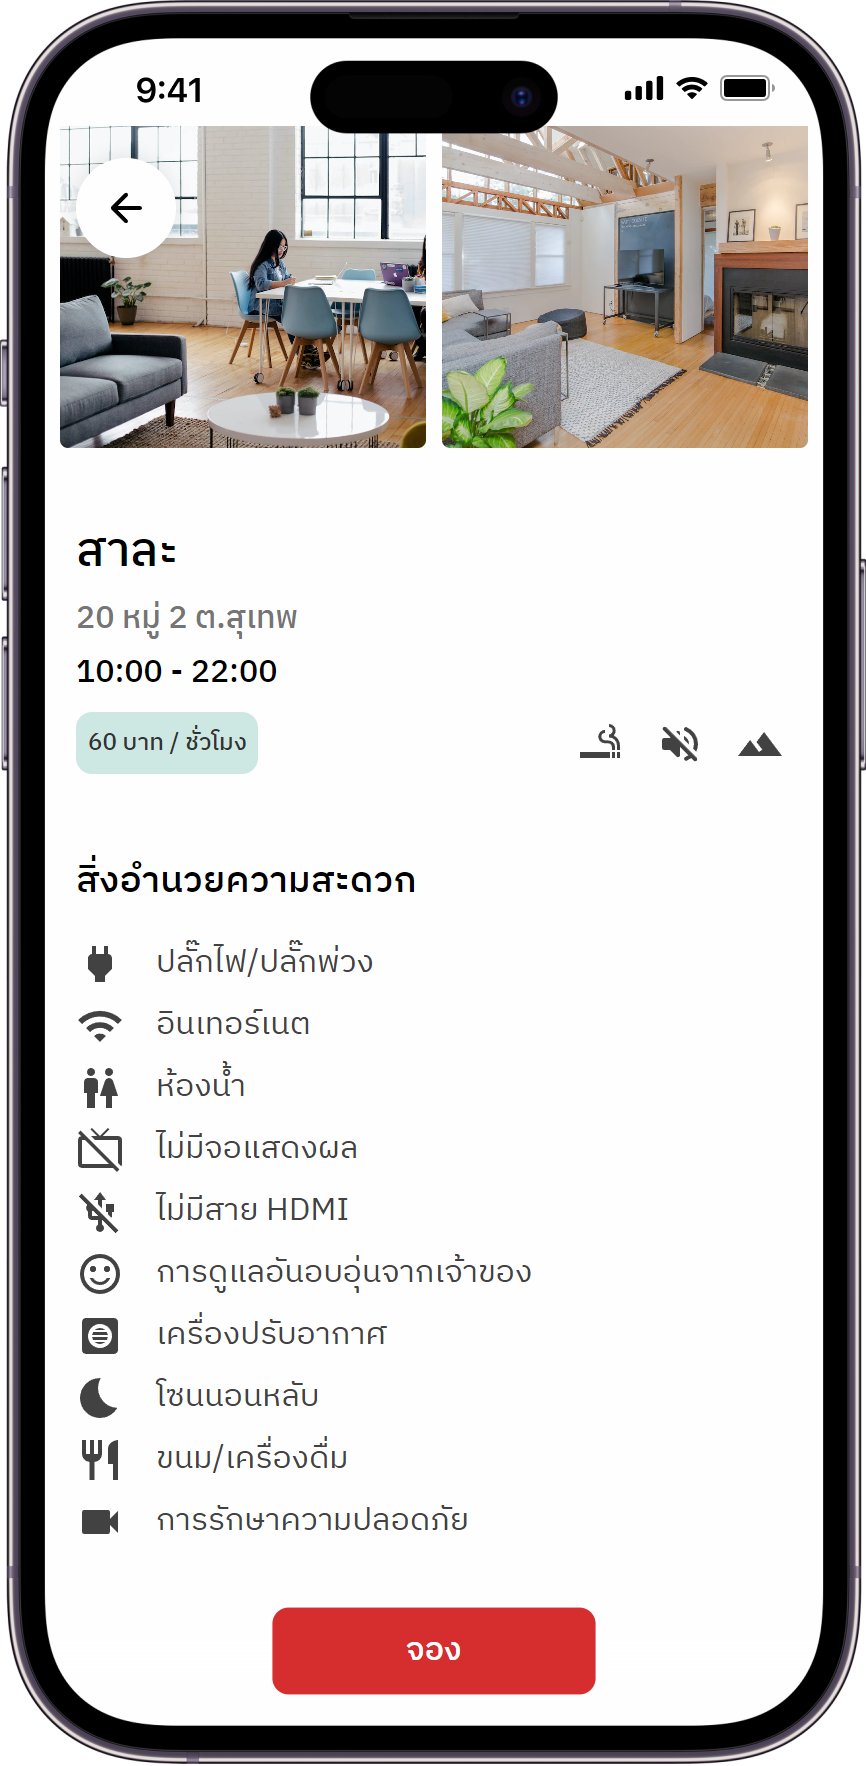
\includegraphics[width=1.9in]{./image/Flowy_info_2.png}
    \end{center}
    \caption[Flowy info 2]{หน้าแสดงรายระเอียดของสเปซ (ต่อ)}
    \label{fig:Flowy_info_2}
\end{figure}
\begin{figure}[ht]
    \begin{center}
    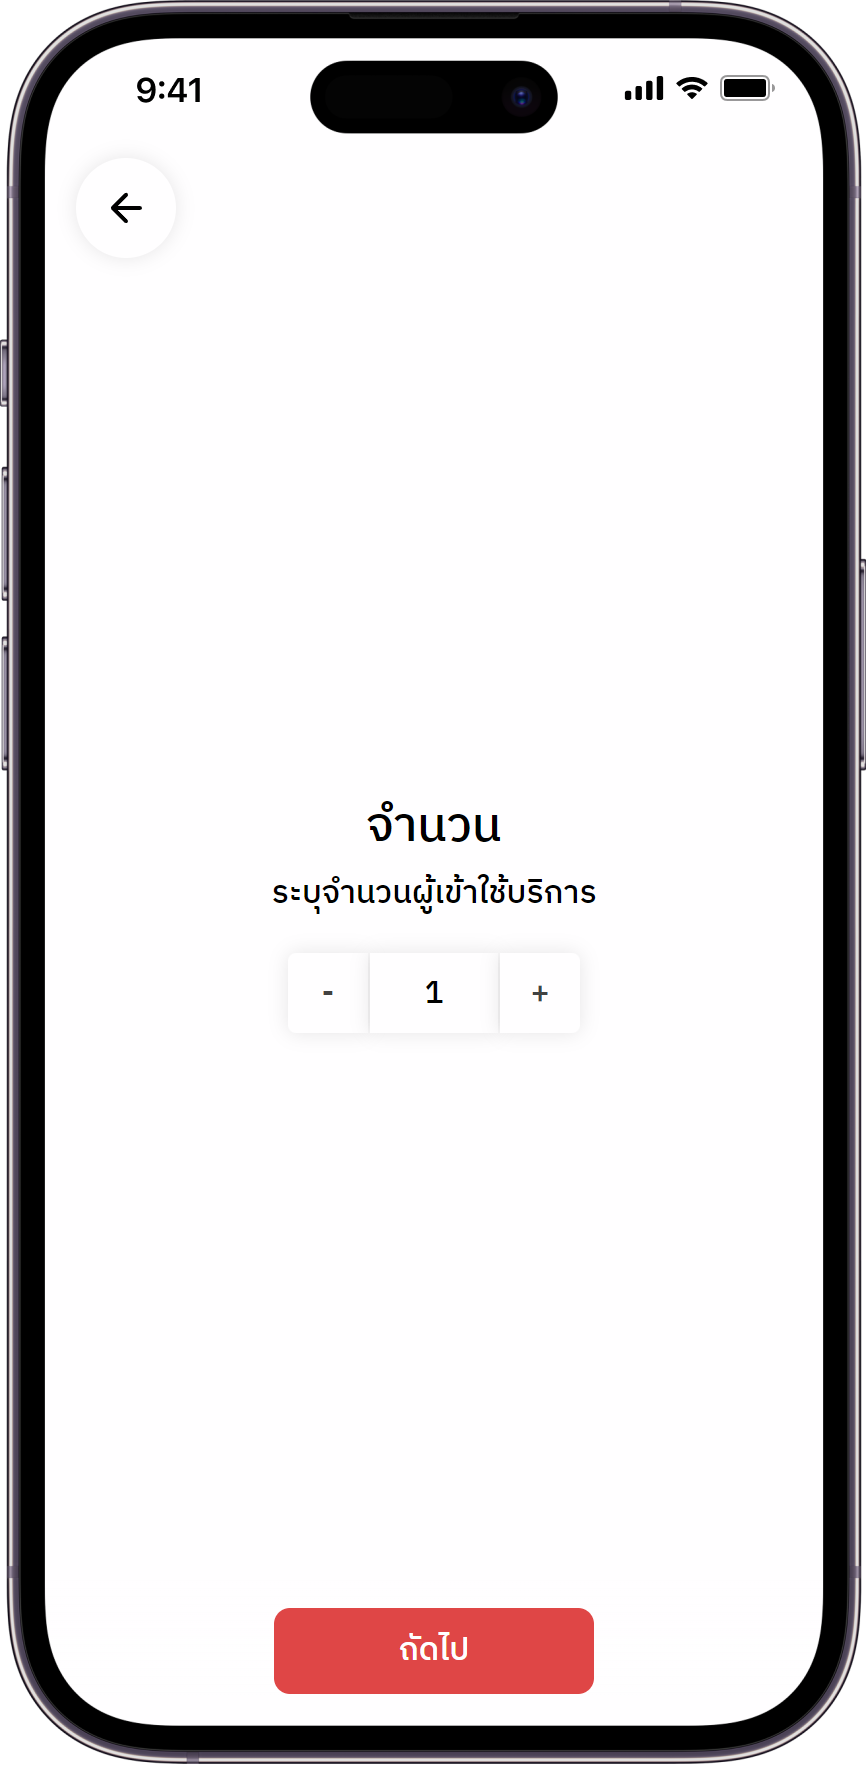
\includegraphics[width=1.9in]{./image/Flowy_book_ctm_amt.png}
    \end{center}
    \caption[Flowy booking customer amount]{หน้าระบุจำนวนผู้เข้าใช้บริการ}
    \label{fig:Flowy_book_ctm_amt}
\end{figure}
\begin{figure}[ht]
    \begin{center}
    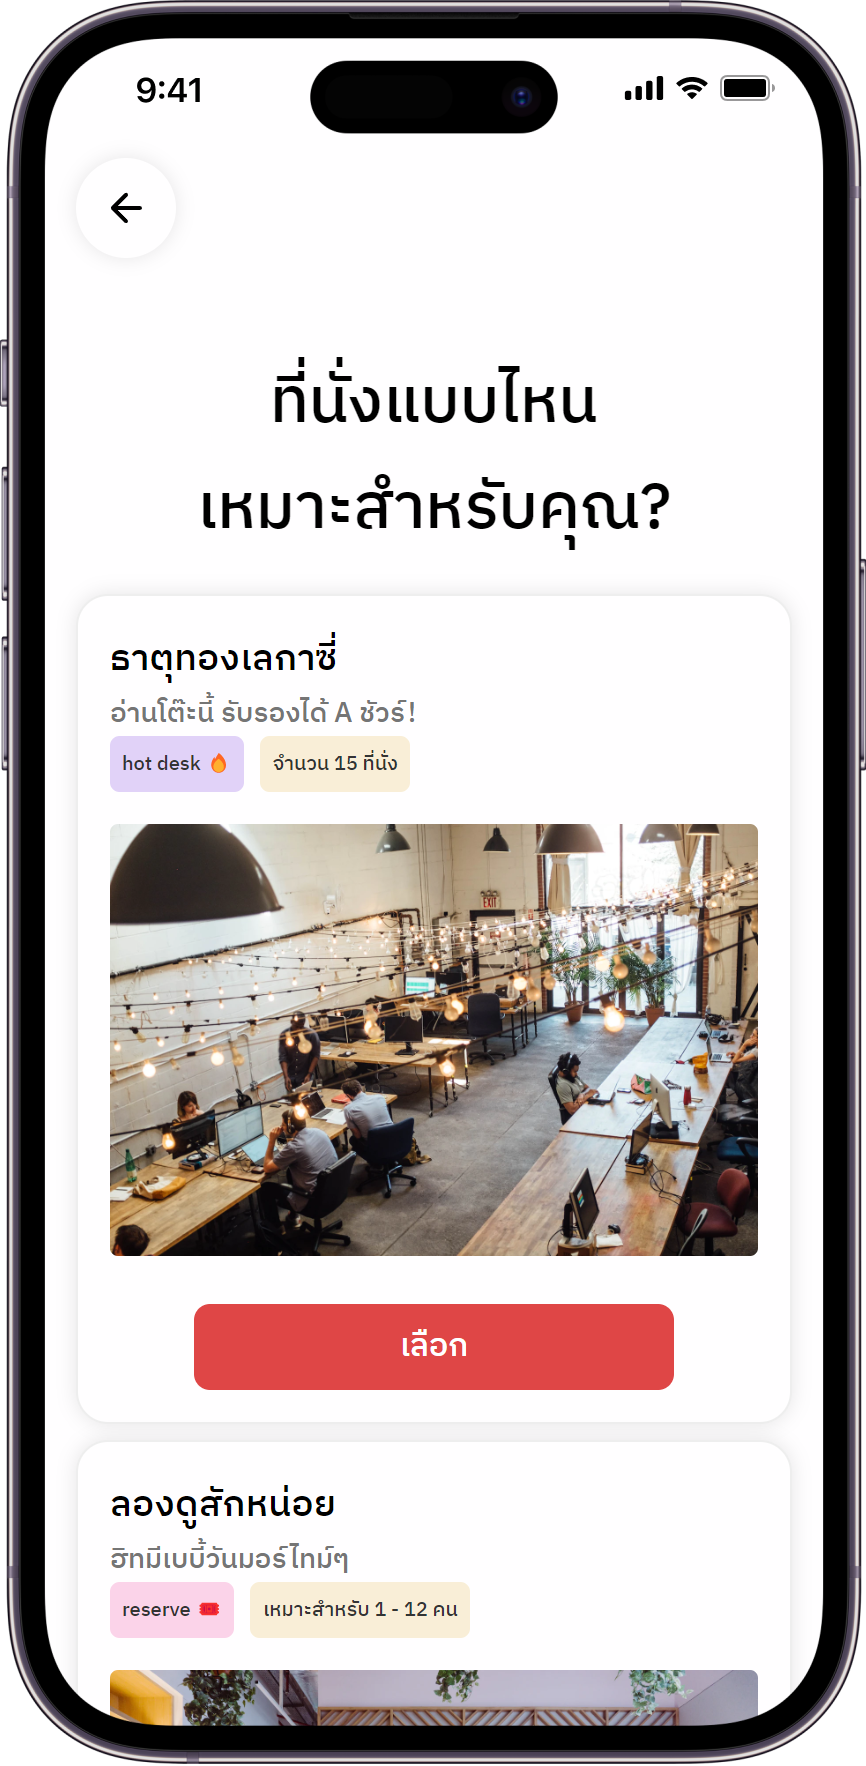
\includegraphics[width=1.9in]{./image/Flowy_book_desk.png}
    \end{center}
    \caption[Flowy booking desk]{หน้าเลือกโต๊ะสำหรับทำกิจกรรมต่าง ๆ}
    \label{fig:Flowy_book_desk}
\end{figure}
\begin{figure}[ht]
    \begin{center}
    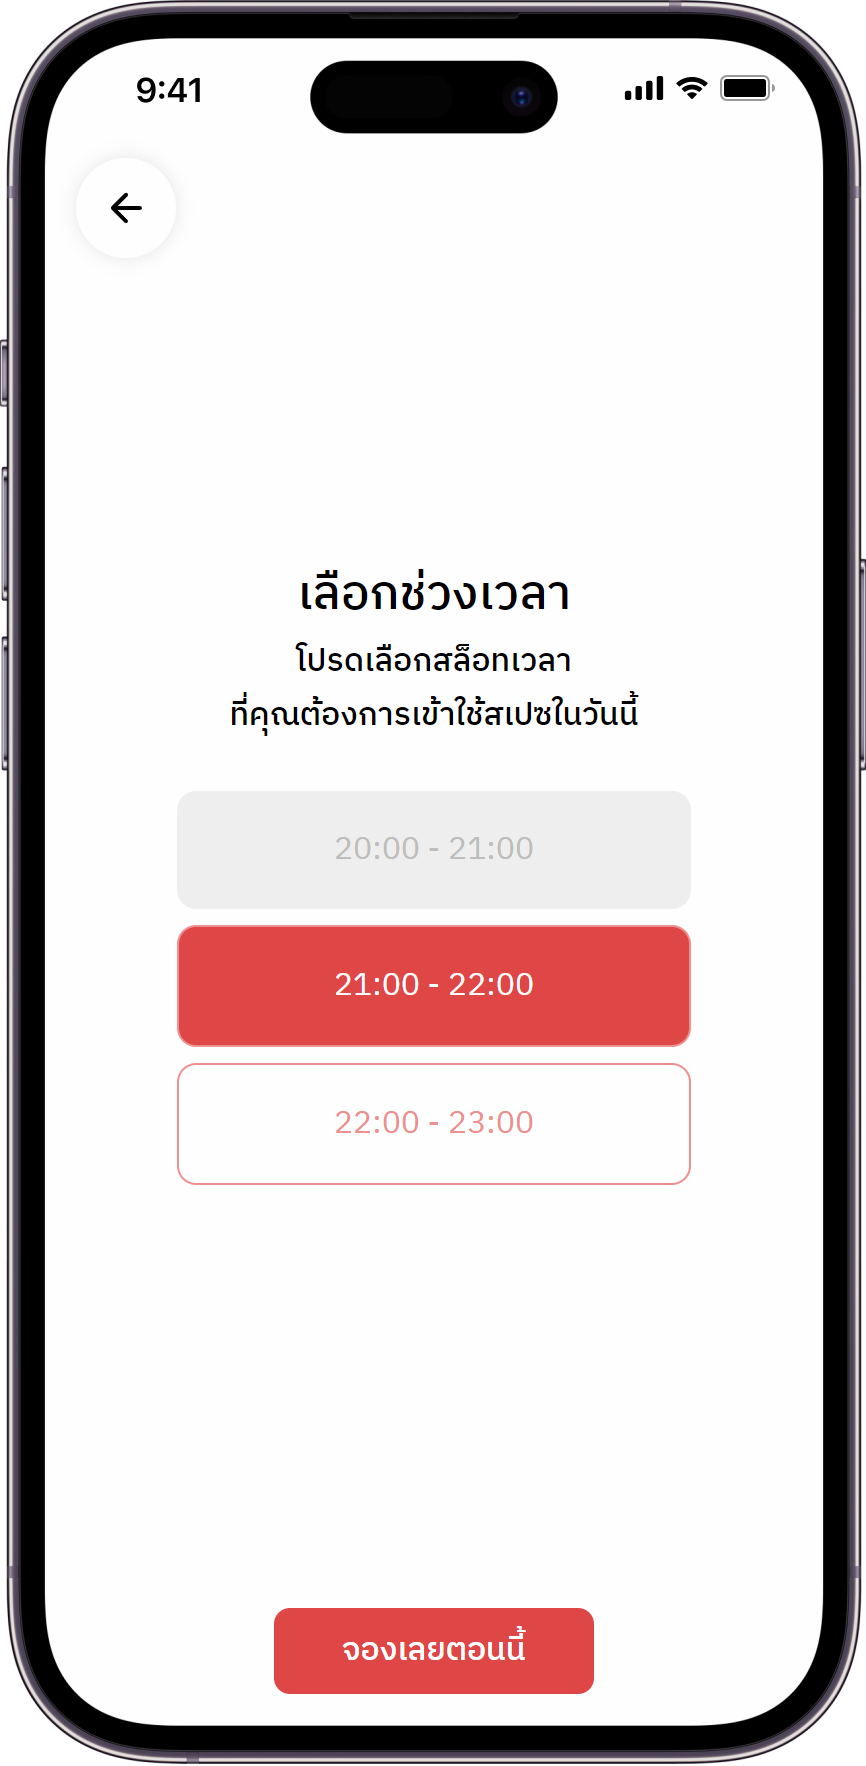
\includegraphics[width=1.9in]{./image/Flowy_book_time_slot.png}
    \end{center}
    \caption[Flowy book time slot]{หน้าระบุเวลาเข้าใช้บริการ}
    \label{fig:Flowy_book_time_slot}
\end{figure}
\begin{figure}[ht]
    \begin{center}
    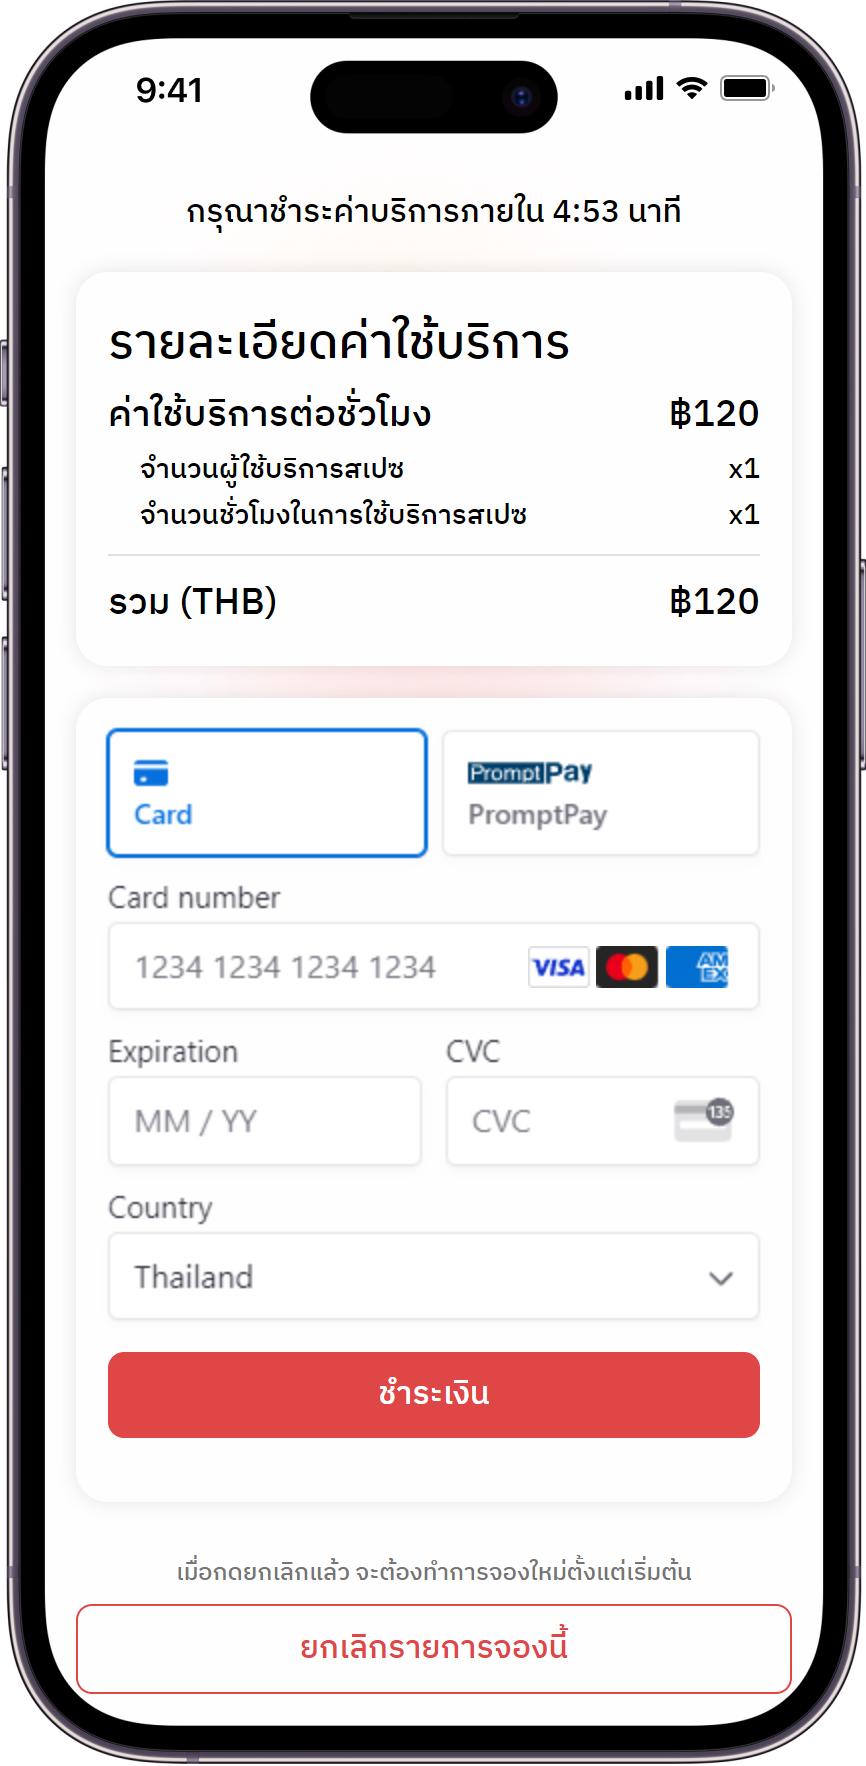
\includegraphics[width=1.9in]{./image/Flowy_payment.png}
    \end{center}
    \caption[Flowy payment]{หน้าชำระค่าบริการ}
    \label{fig:Flowy_payment}
\end{figure}
\begin{figure}[ht]
    \begin{center}
    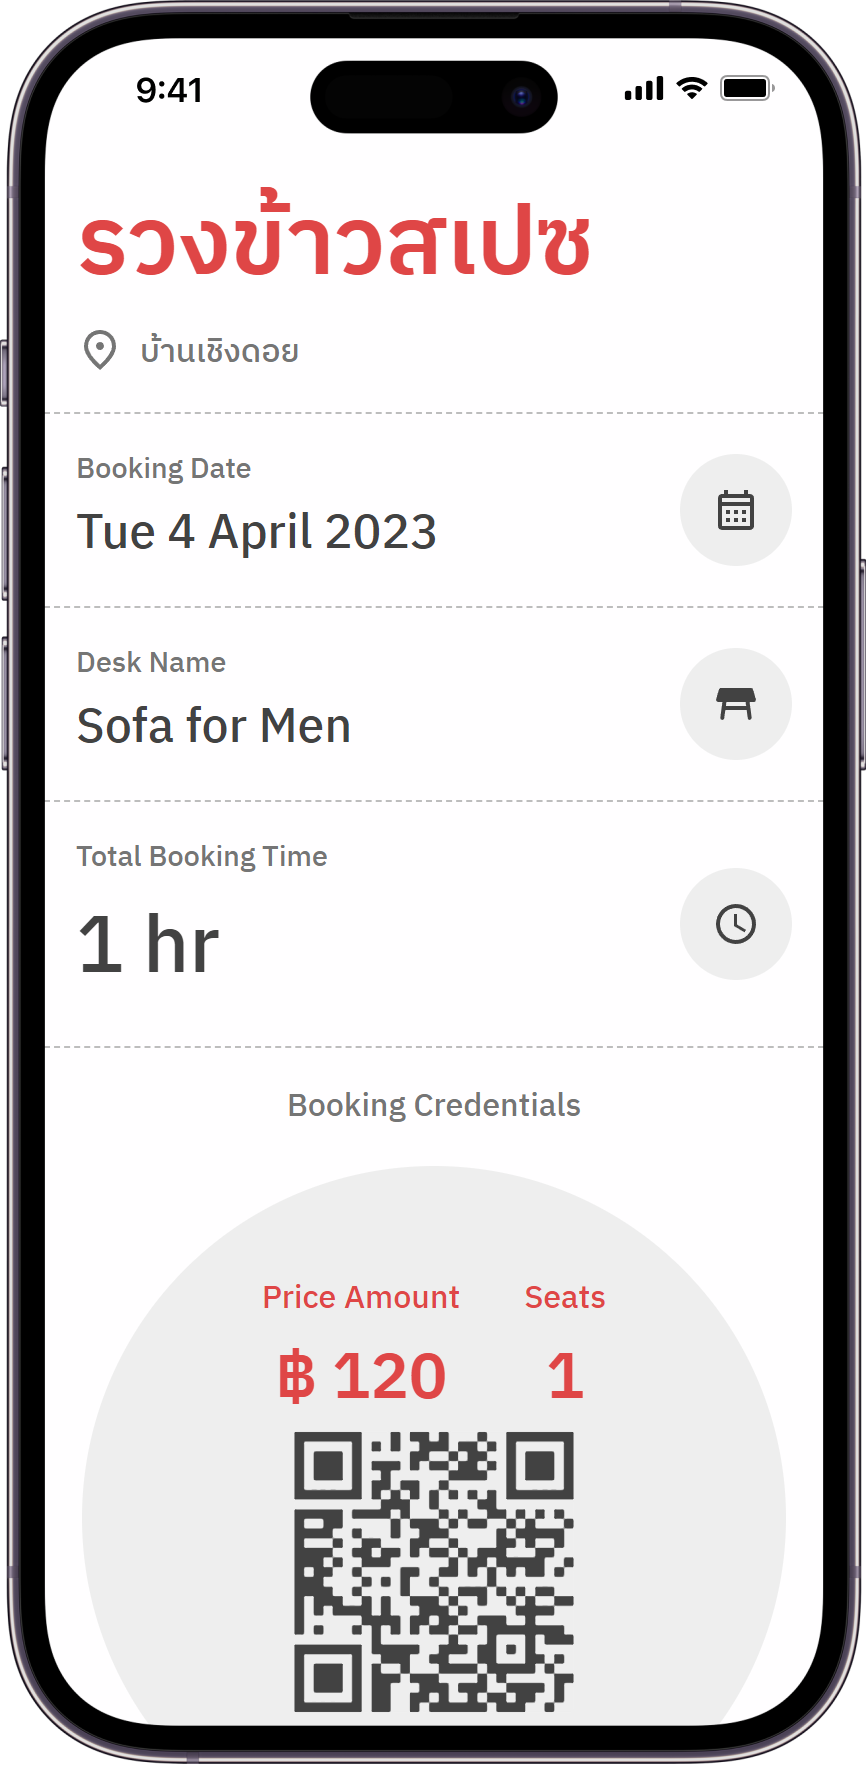
\includegraphics[width=1.9in]{./image/Flowy_ticket_1.png}
    \end{center}
    \caption[Flowy ticket 1]{หน้าแสดงรายระเอียดตั๋ว}
    \label{fig:Flowy_ticket_1}
\end{figure}
\begin{figure}[ht]
    \begin{center}
    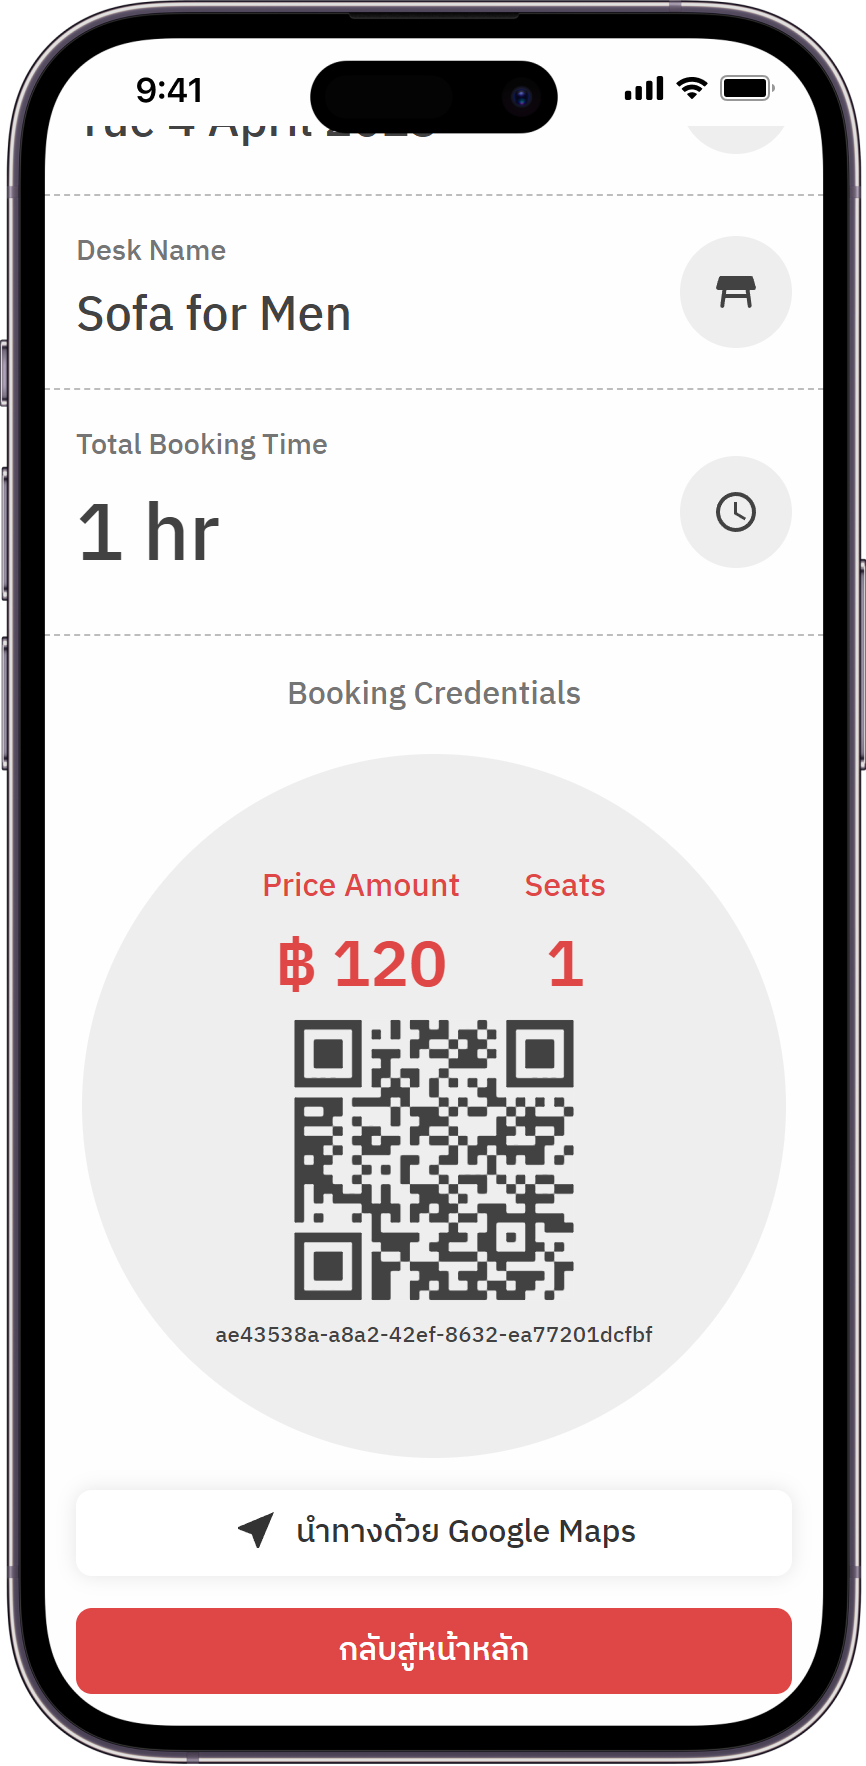
\includegraphics[width=1.9in]{./image/Flowy_ticket_2.png}
    \end{center}
    \caption[Flowy ticket 2]{หน้าแสดงรายระเอียดตั๋ว (ต่อ)}
    \label{fig:Flowy_ticket_2}
\end{figure}
\begin{figure}[ht]
    \begin{center}
    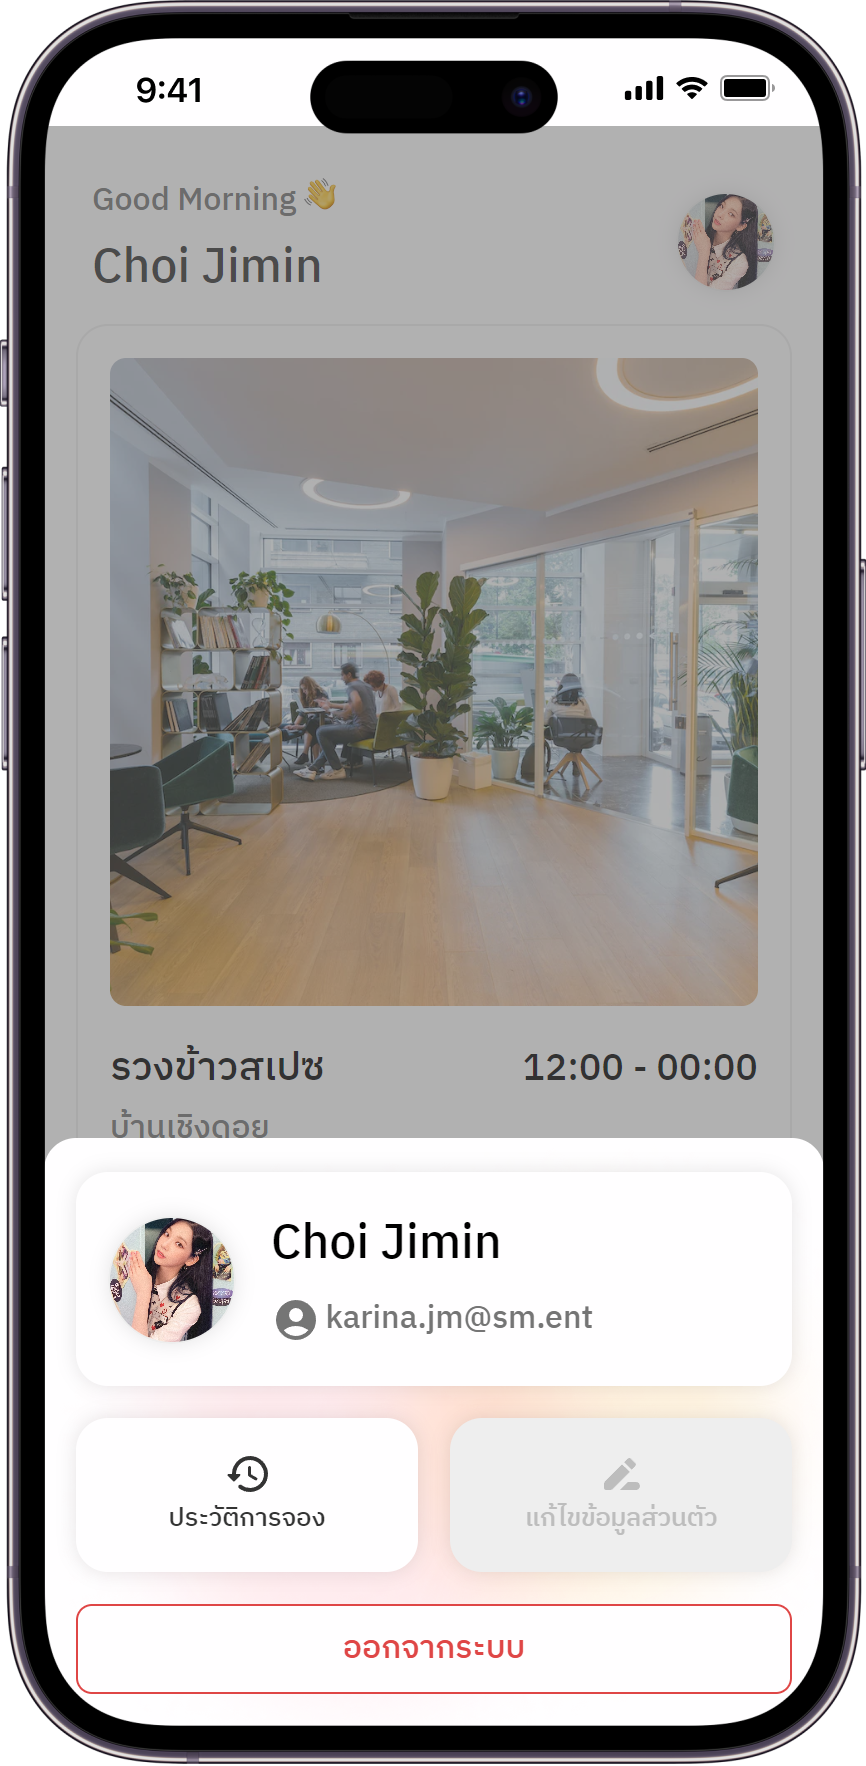
\includegraphics[width=1.9in]{./image/Flowy_account.png}
    \end{center}
    \caption[Flowy account]{หน้าแสดงบัญชีผู้ใช้ (Flowy)}
    \label{fig:Flowy_account}
\end{figure}
\begin{figure}[ht]
    \begin{center}
    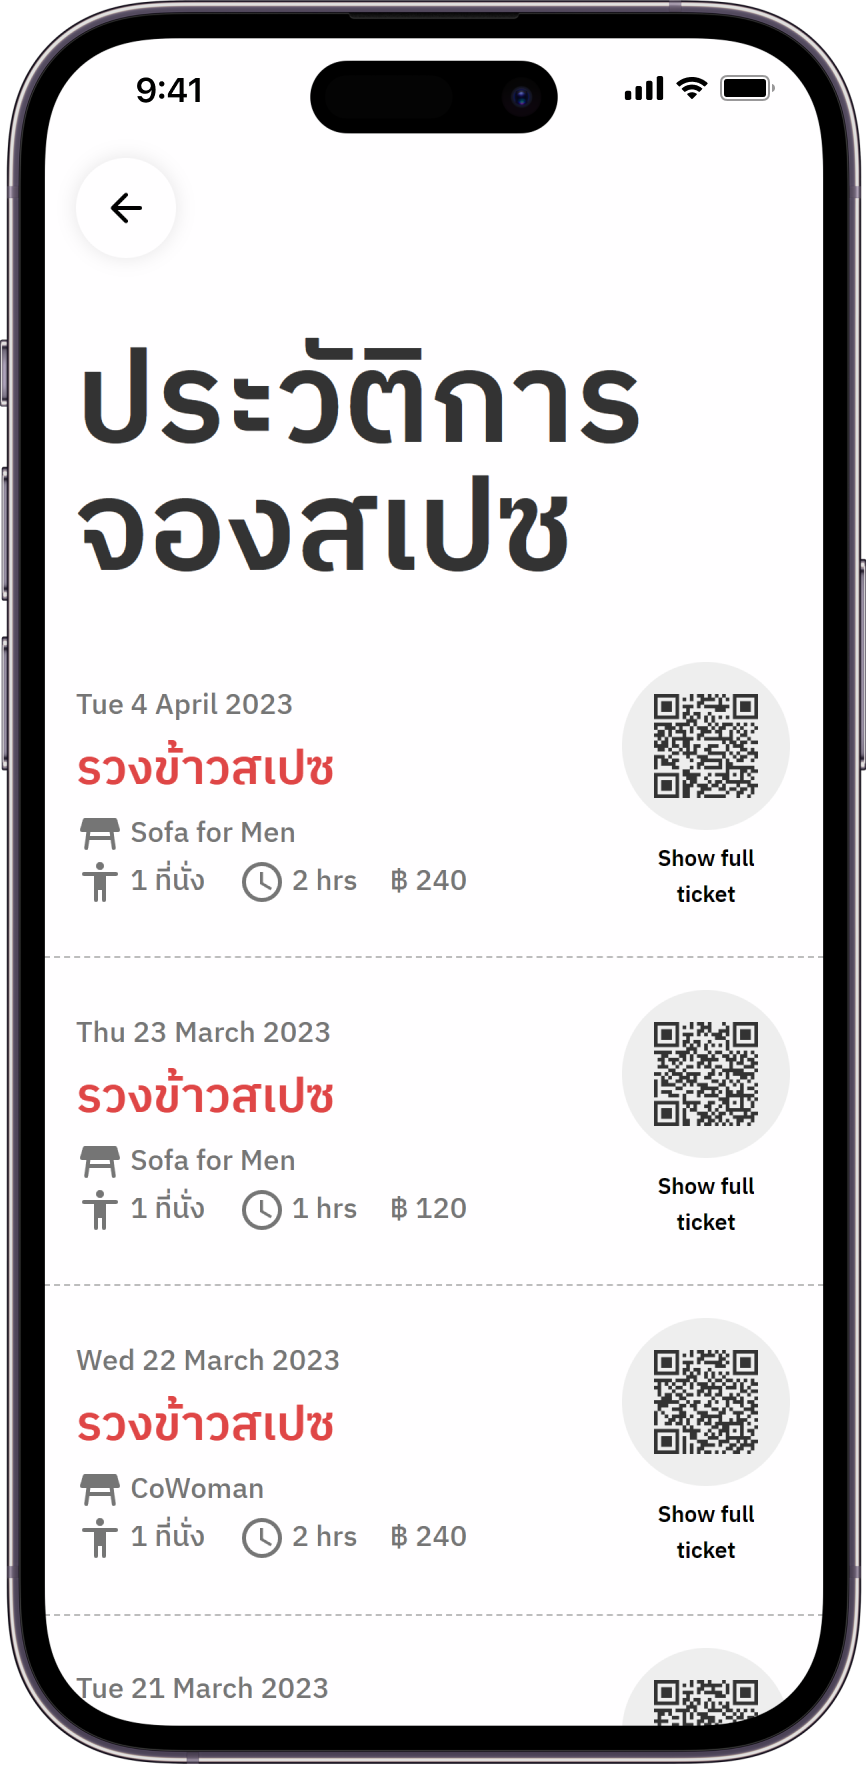
\includegraphics[width=1.9in]{./image/Flowy_book_history.png}
    \end{center}
    \caption[Flowy book history]{หน้าแสดงประวิติการจองสเปซ}
    \label{fig:Flowy_book_history}
\end{figure}
\begin{figure}[ht]
    \begin{center}
    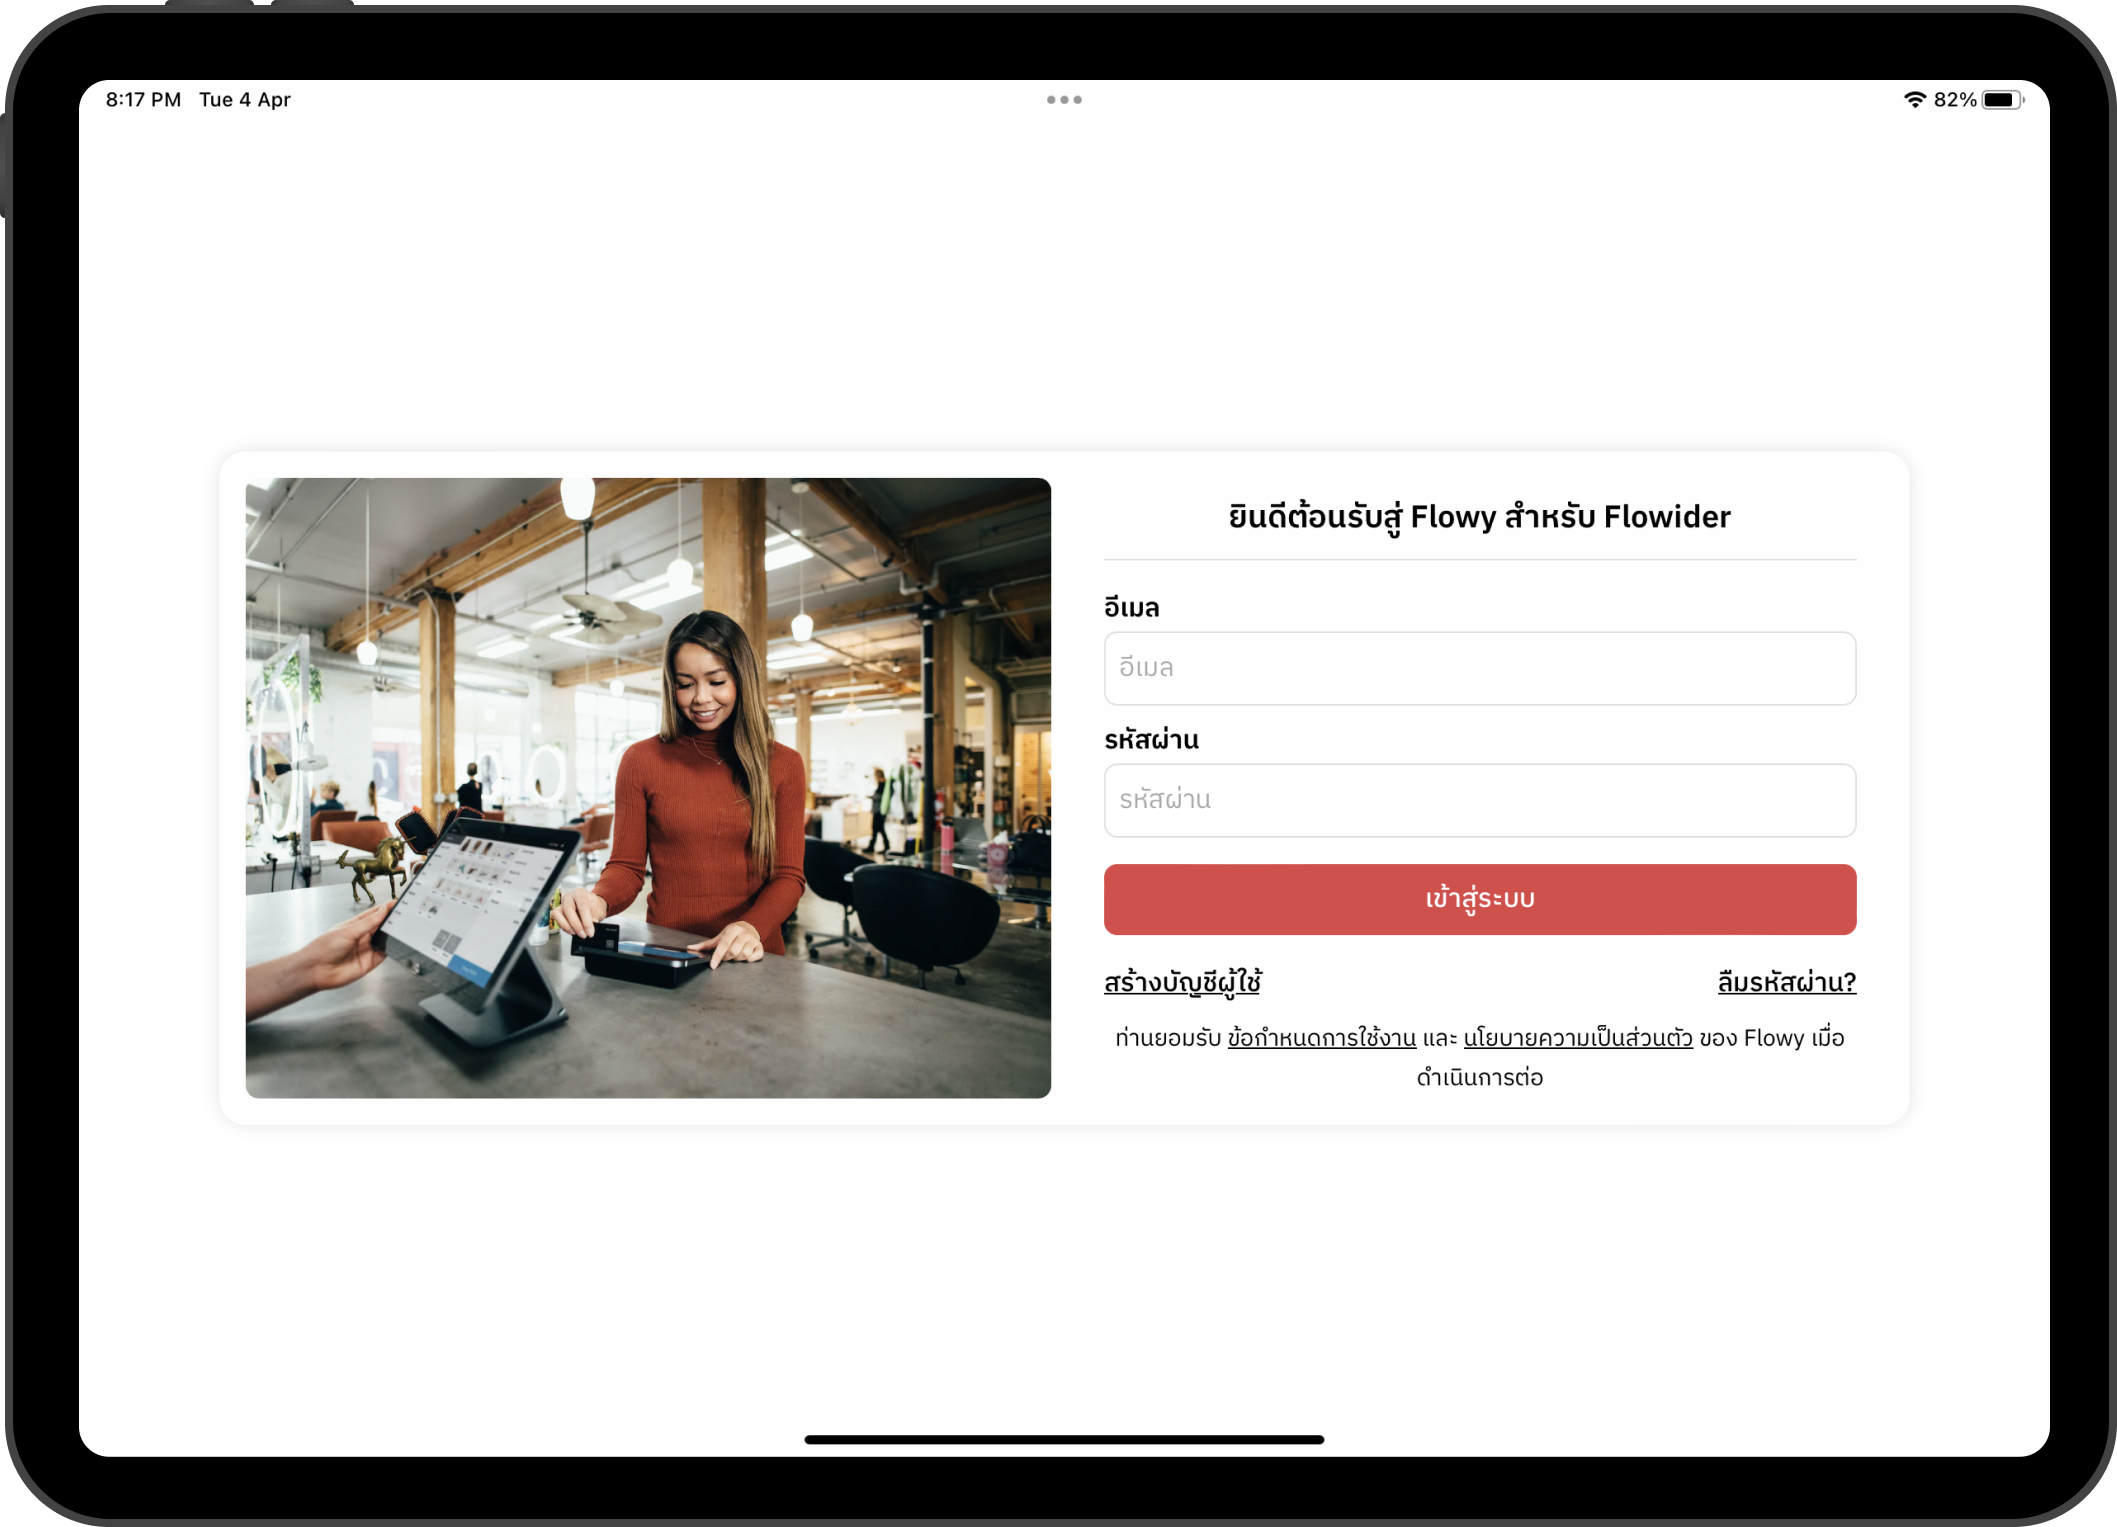
\includegraphics[width=5.5in]{./image/Flowider_login.png}
    \end{center}
    \caption[Flowider login]{หน้าเข้าสู่ระบบสำหรับผู้ใช้งาน (Flowider)}
    \label{fig:Flowider_login}
\end{figure}
\begin{figure}[ht]
    \begin{center}
    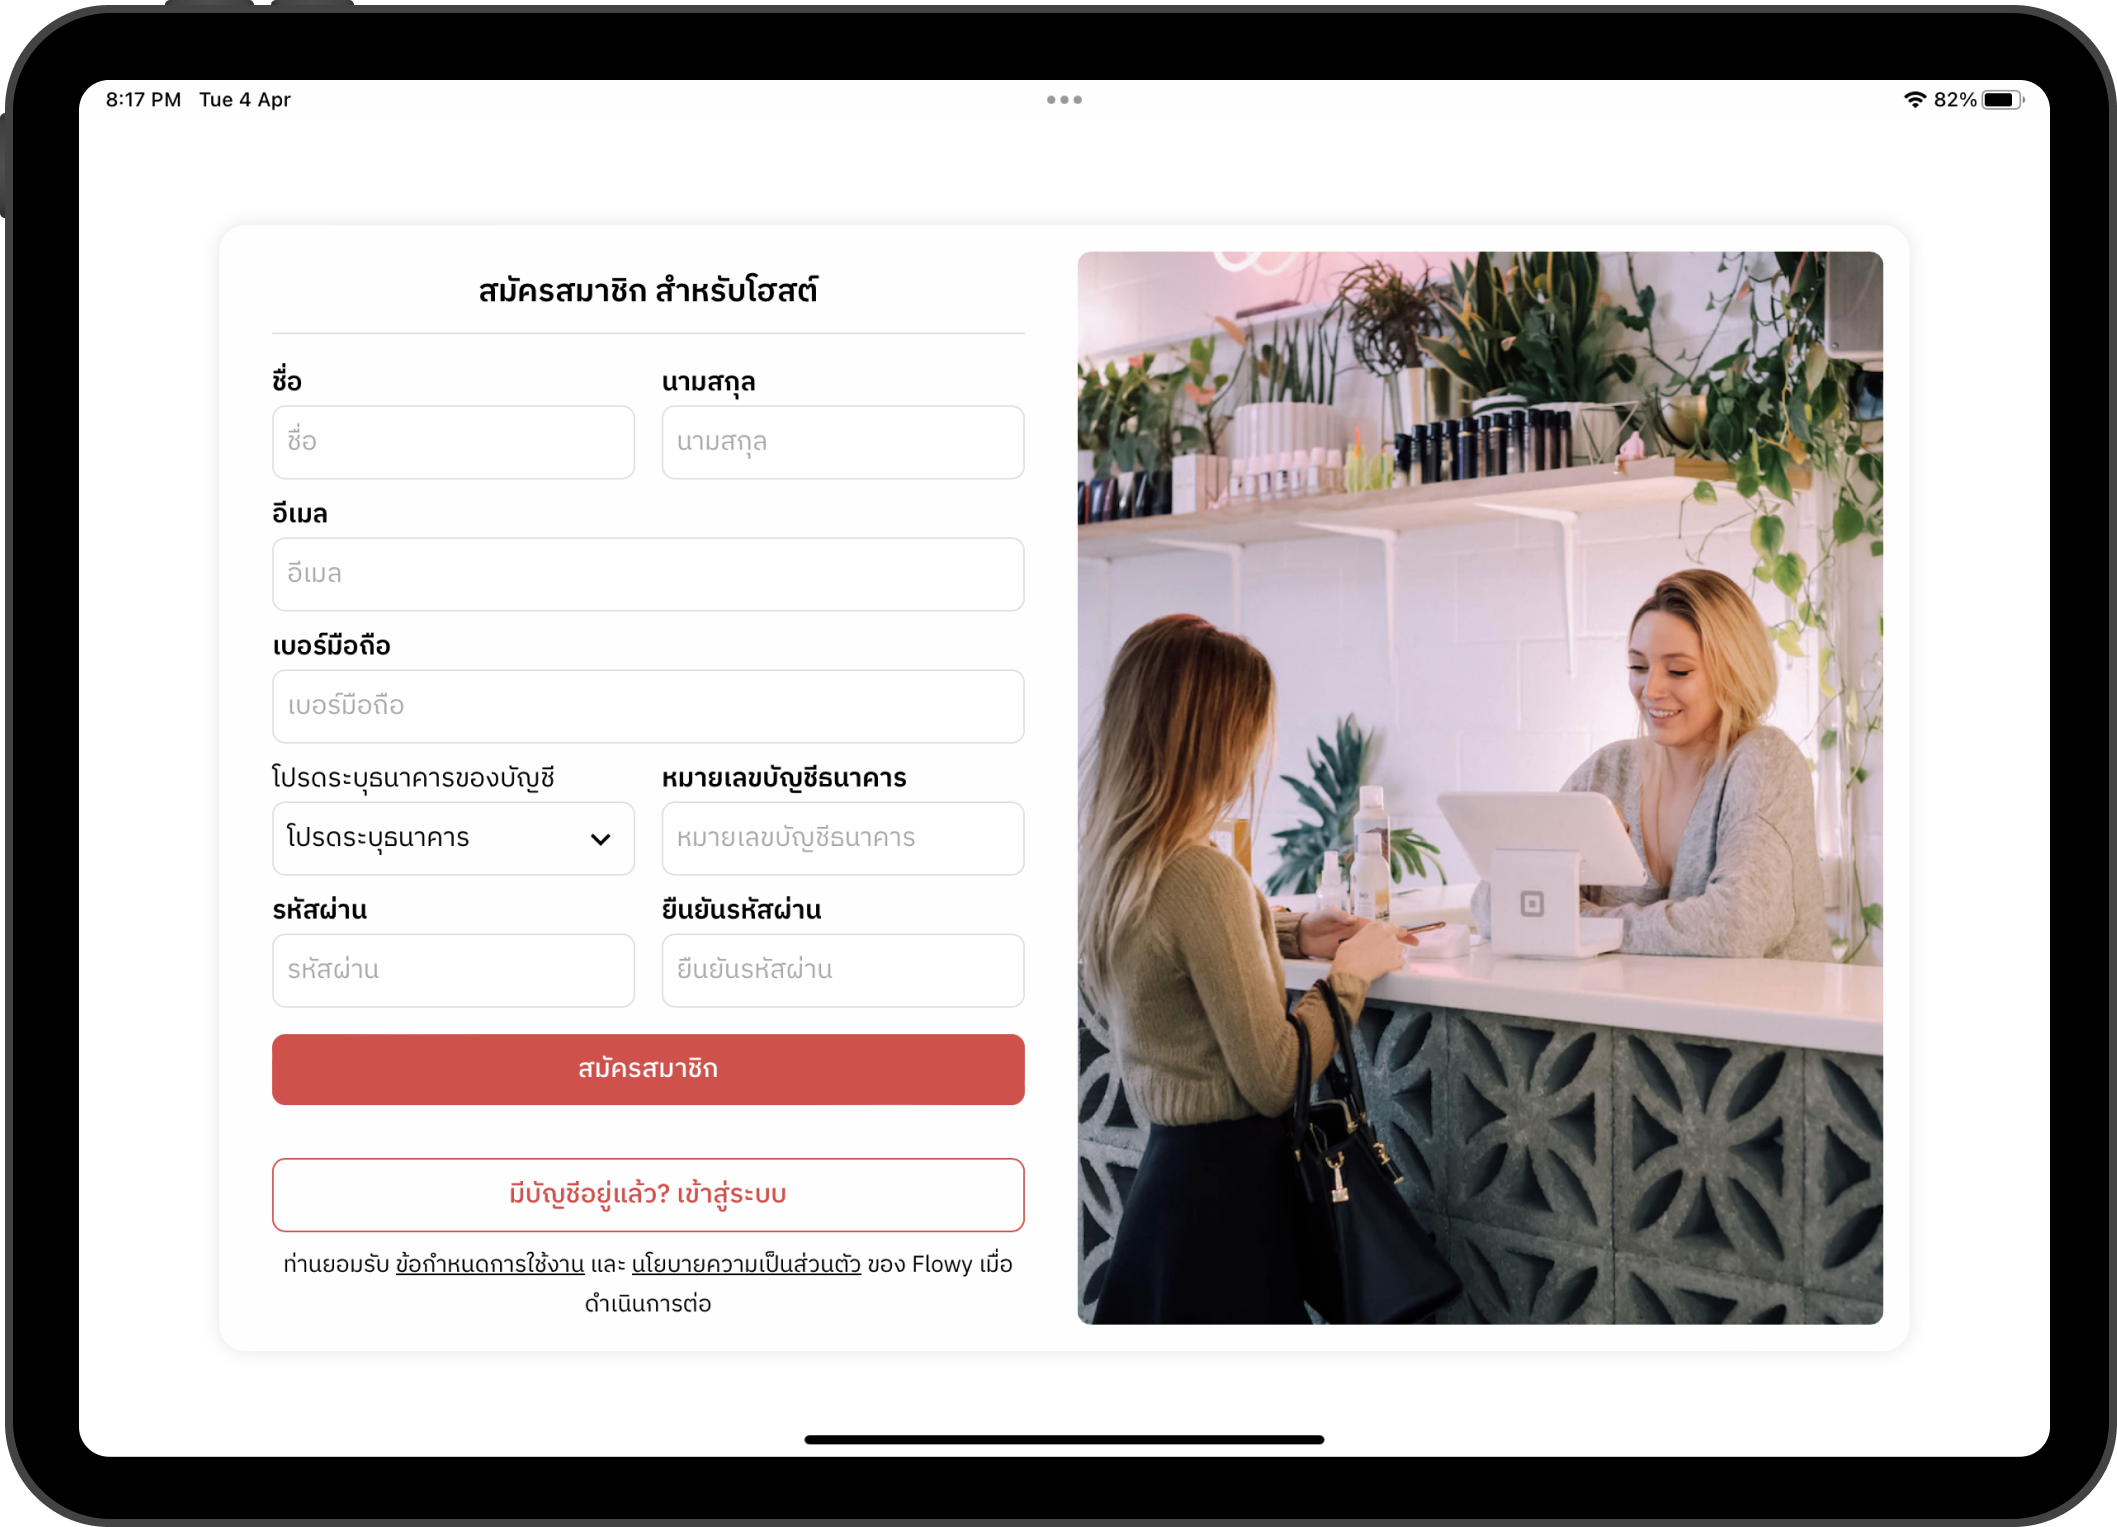
\includegraphics[width=5.5in]{./image/Flowider_register.png}
    \end{center}
    \caption[Flowider register]{หน้าสมัครสมาชิกสำหรับผู้ใช้งาน (Flowider)}
    \label{fig:Flowider_register}
\end{figure}
\begin{figure}[ht]
    \begin{center}
    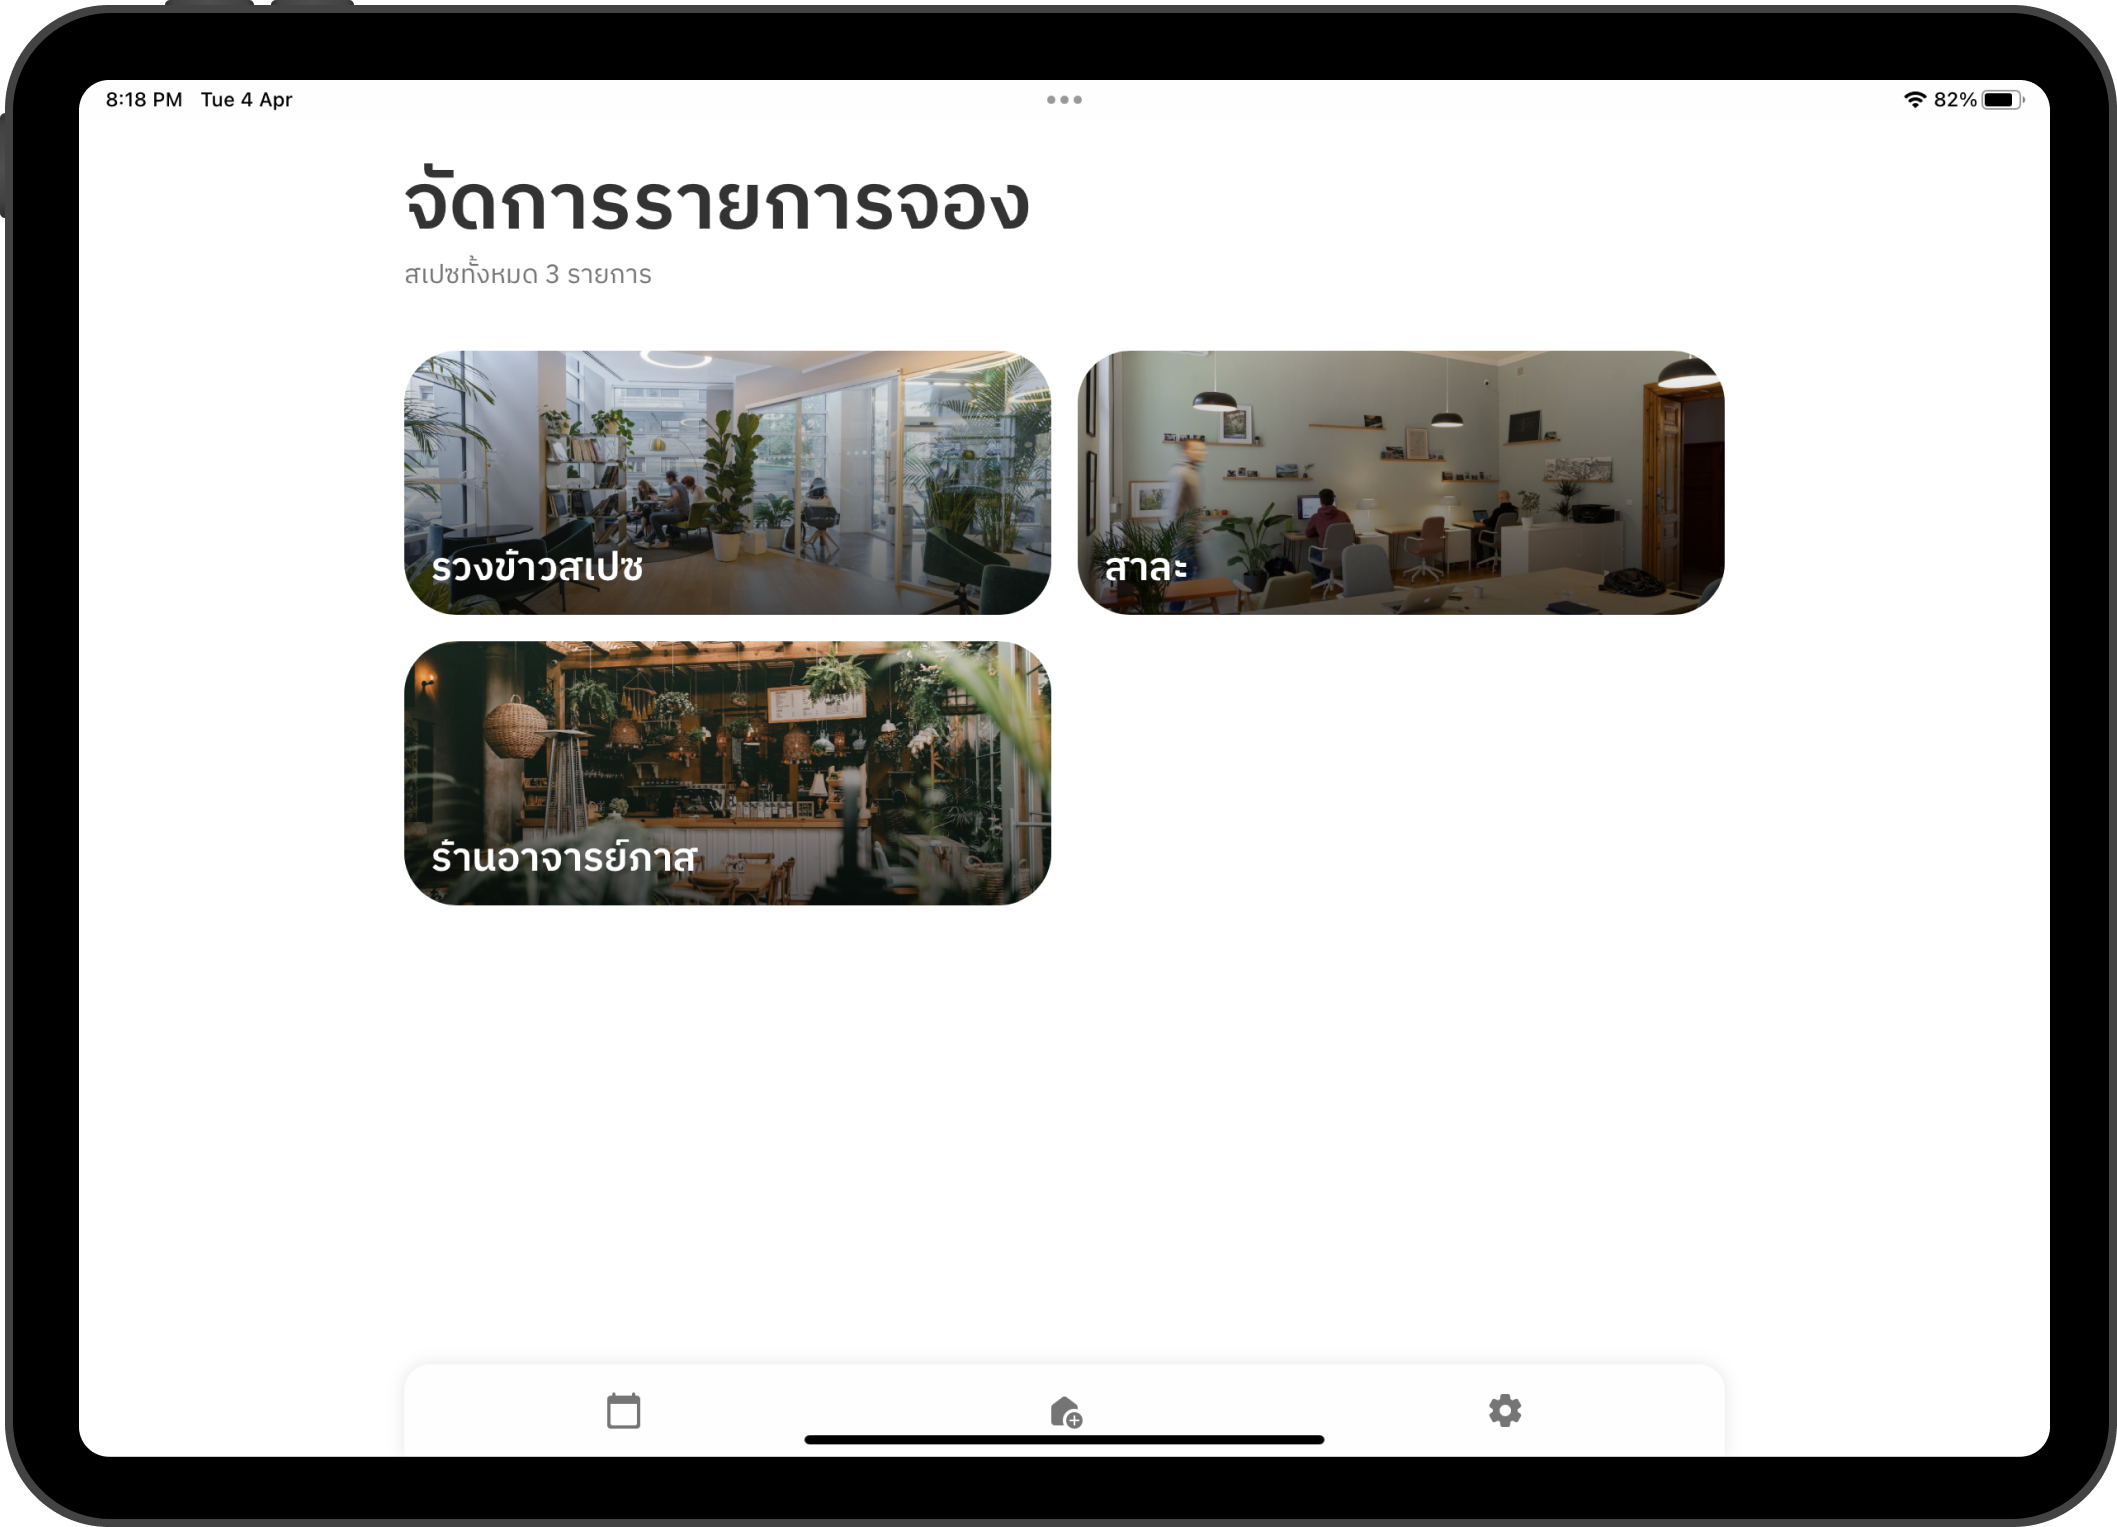
\includegraphics[width=5.5in]{./image/Flowider_booking_mgmt.png}
    \end{center}
    \caption[Flowider booking management]{หน้าจัดการรายการจอง}
    \label{fig:Flowider_booking_mgmt}
\end{figure}
\begin{figure}[ht]
    \begin{center}
    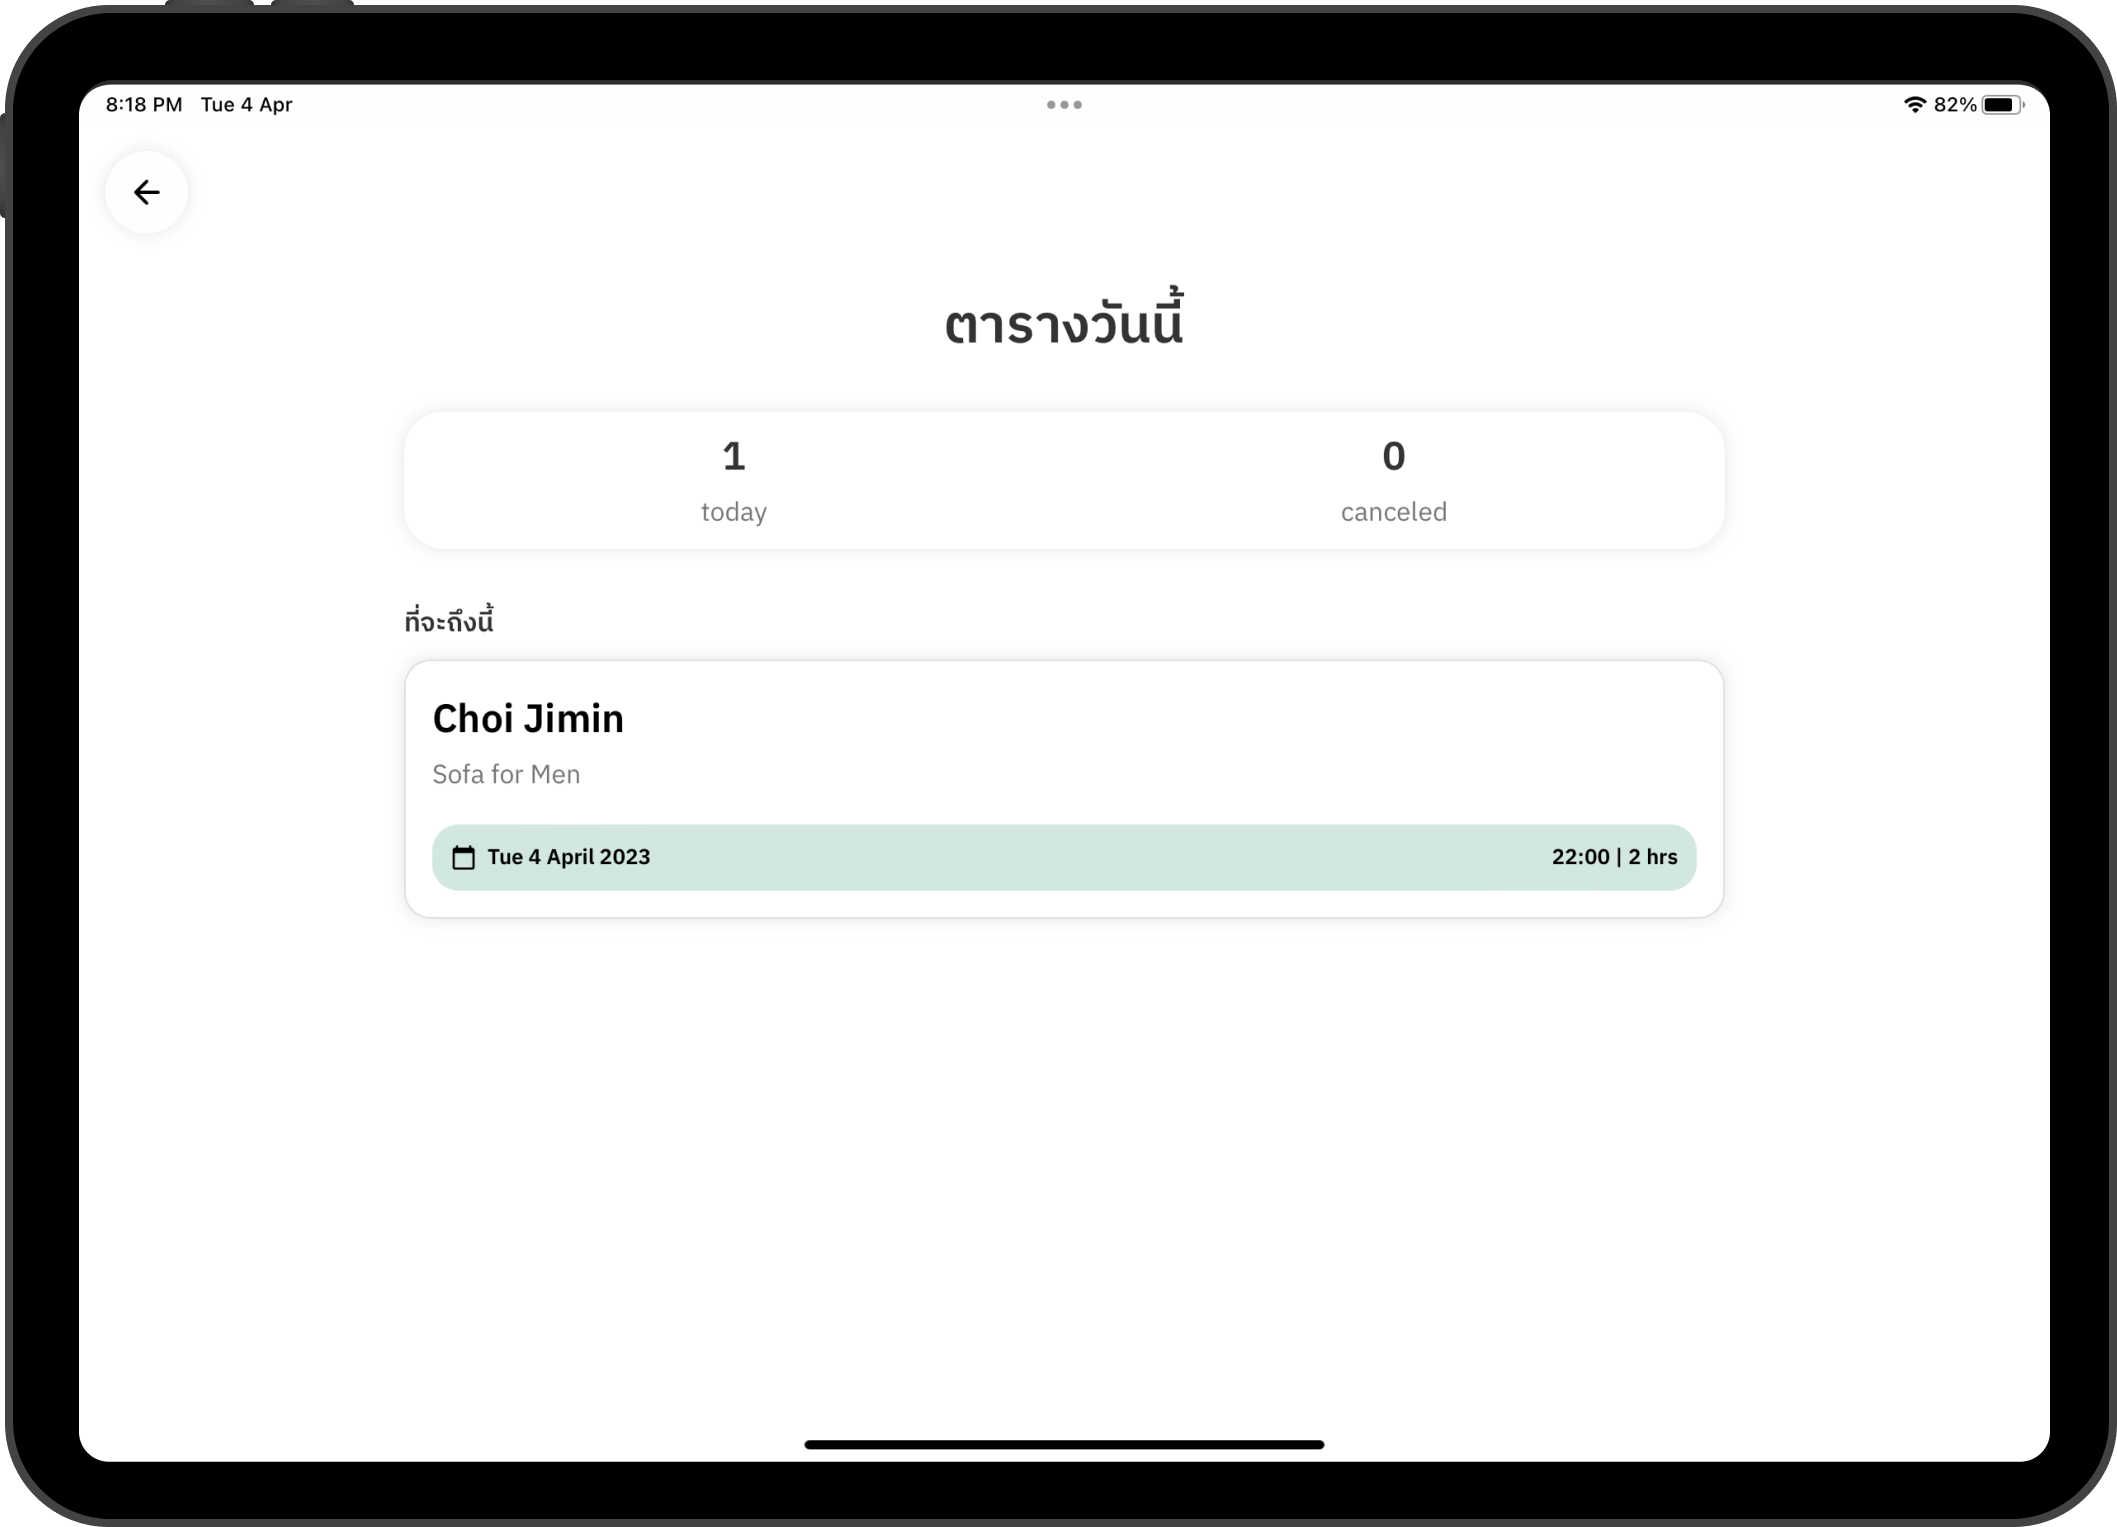
\includegraphics[width=5.5in]{./image/Flowider_schedule.png}
    \end{center}
    \caption[Flowide schedule]{หน้าแสดงรายระเอียดการจองของแต่ละสเปซ}
    \label{fig:Flowider_schedule}
\end{figure}
\begin{figure}[ht]
    \begin{center}
    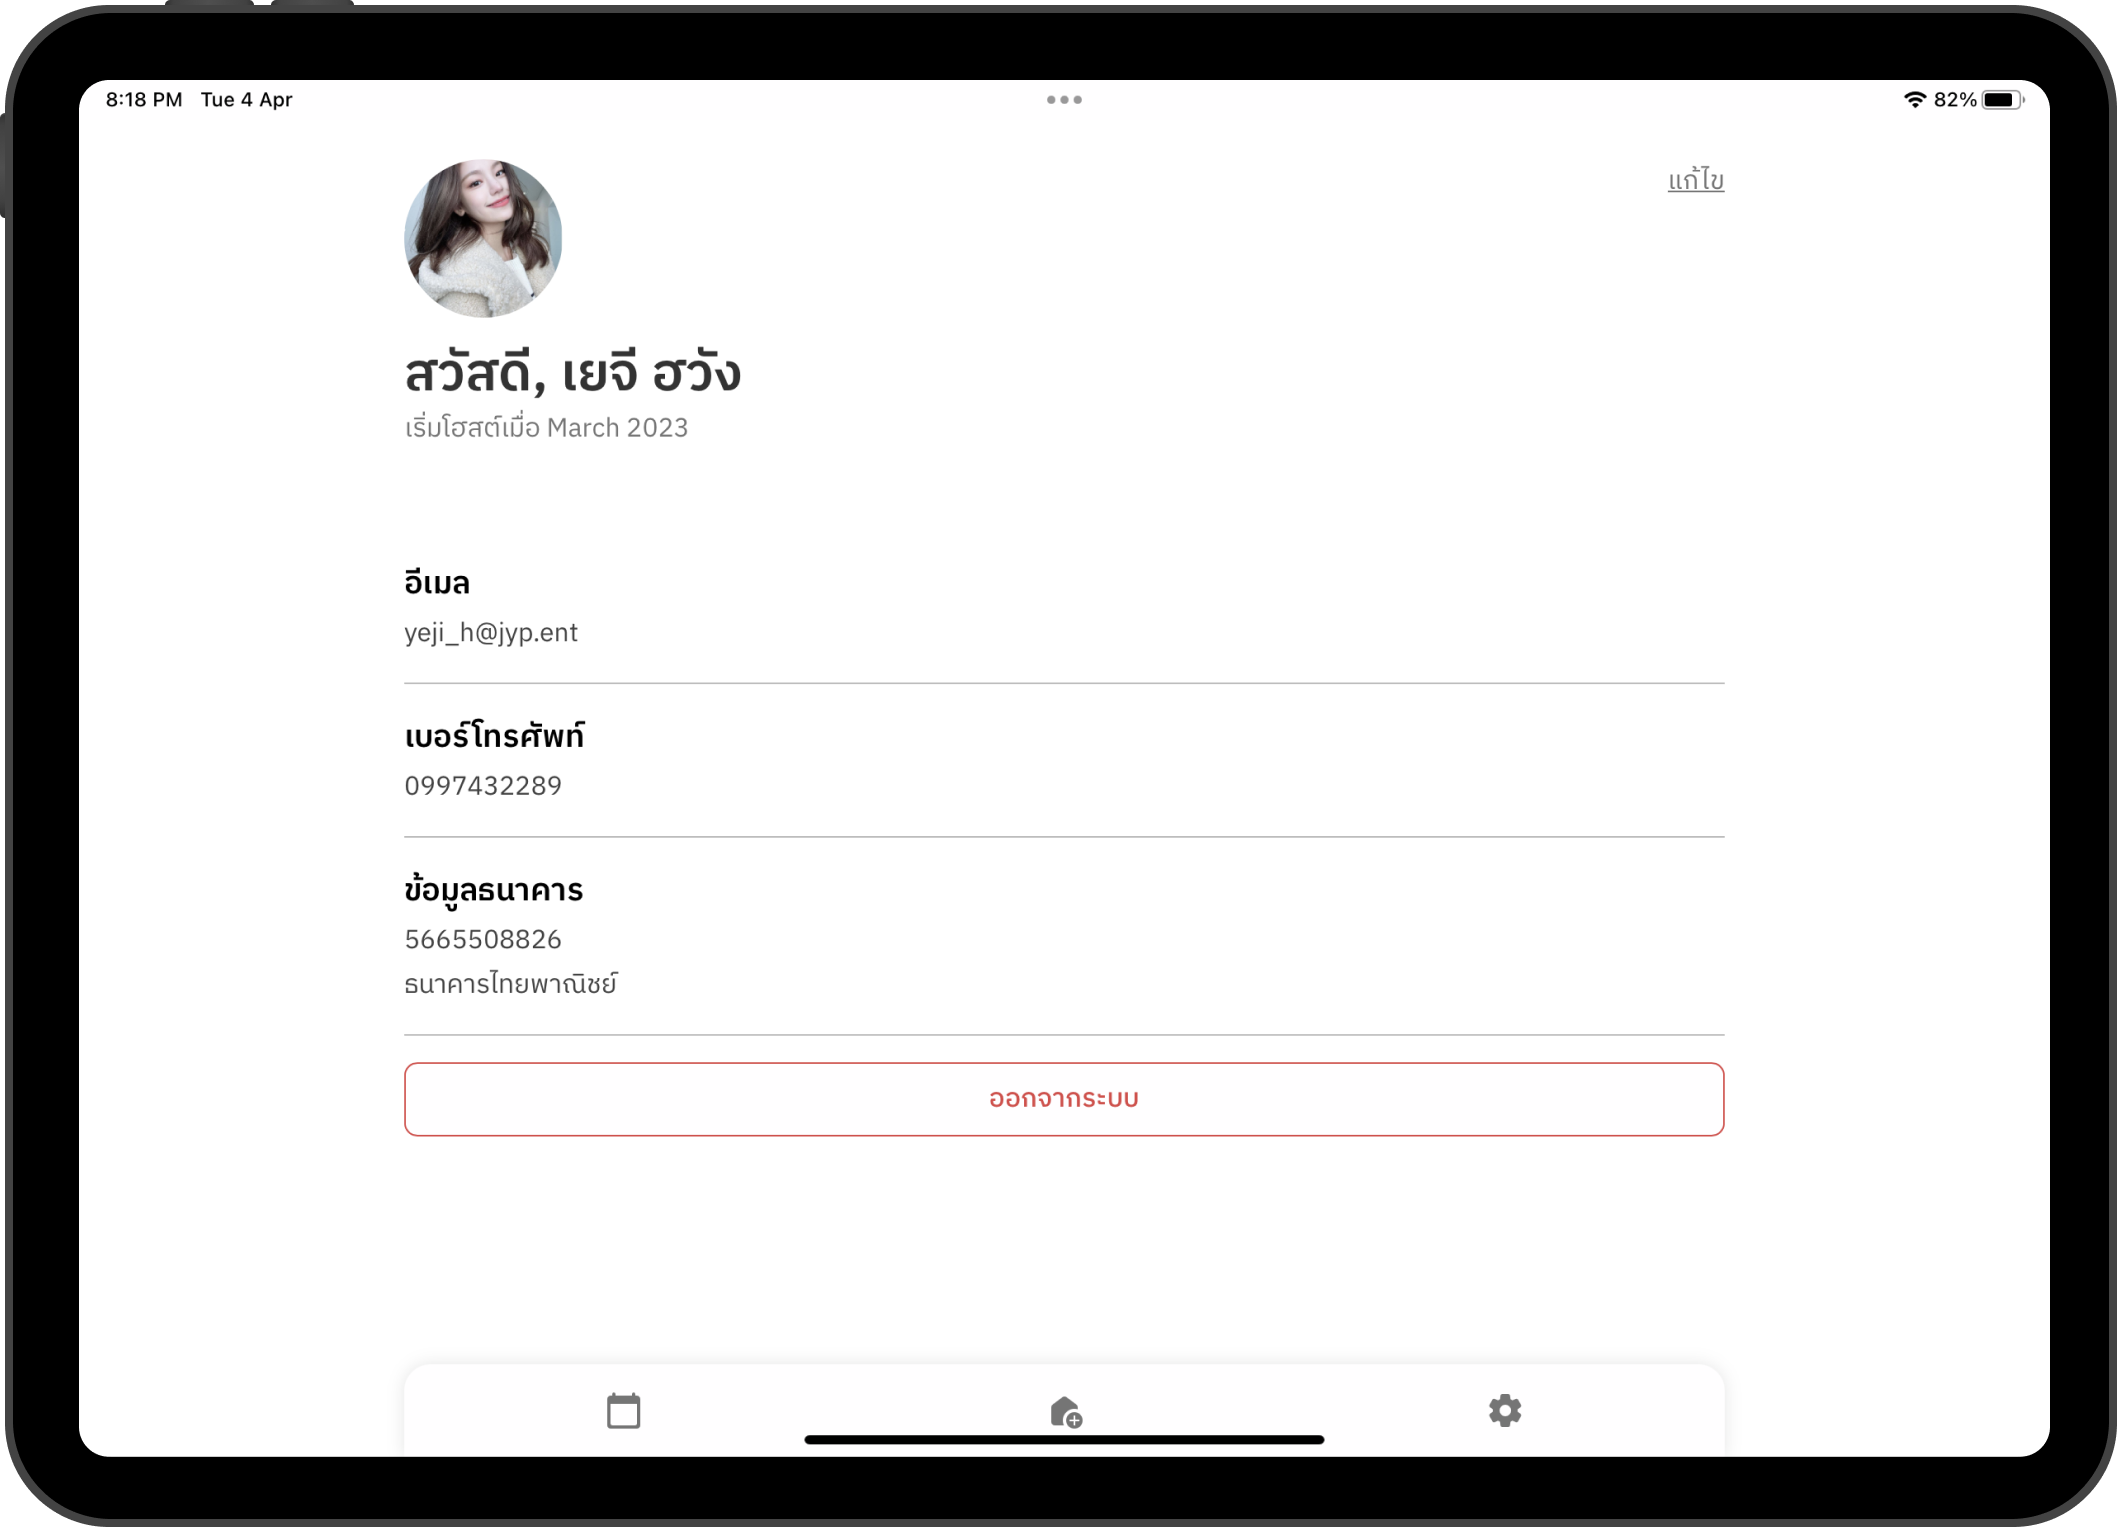
\includegraphics[width=5.5in]{./image/Flowider_account.png}
    \end{center}
    \caption[Flowider account]{หน้าแสดงบัญชีผู้ใช้ของผู้ใช้บริการ (Flowider)}
    \label{fig:Flowider_account}
\end{figure}
\begin{figure}[ht]
    \begin{center}
    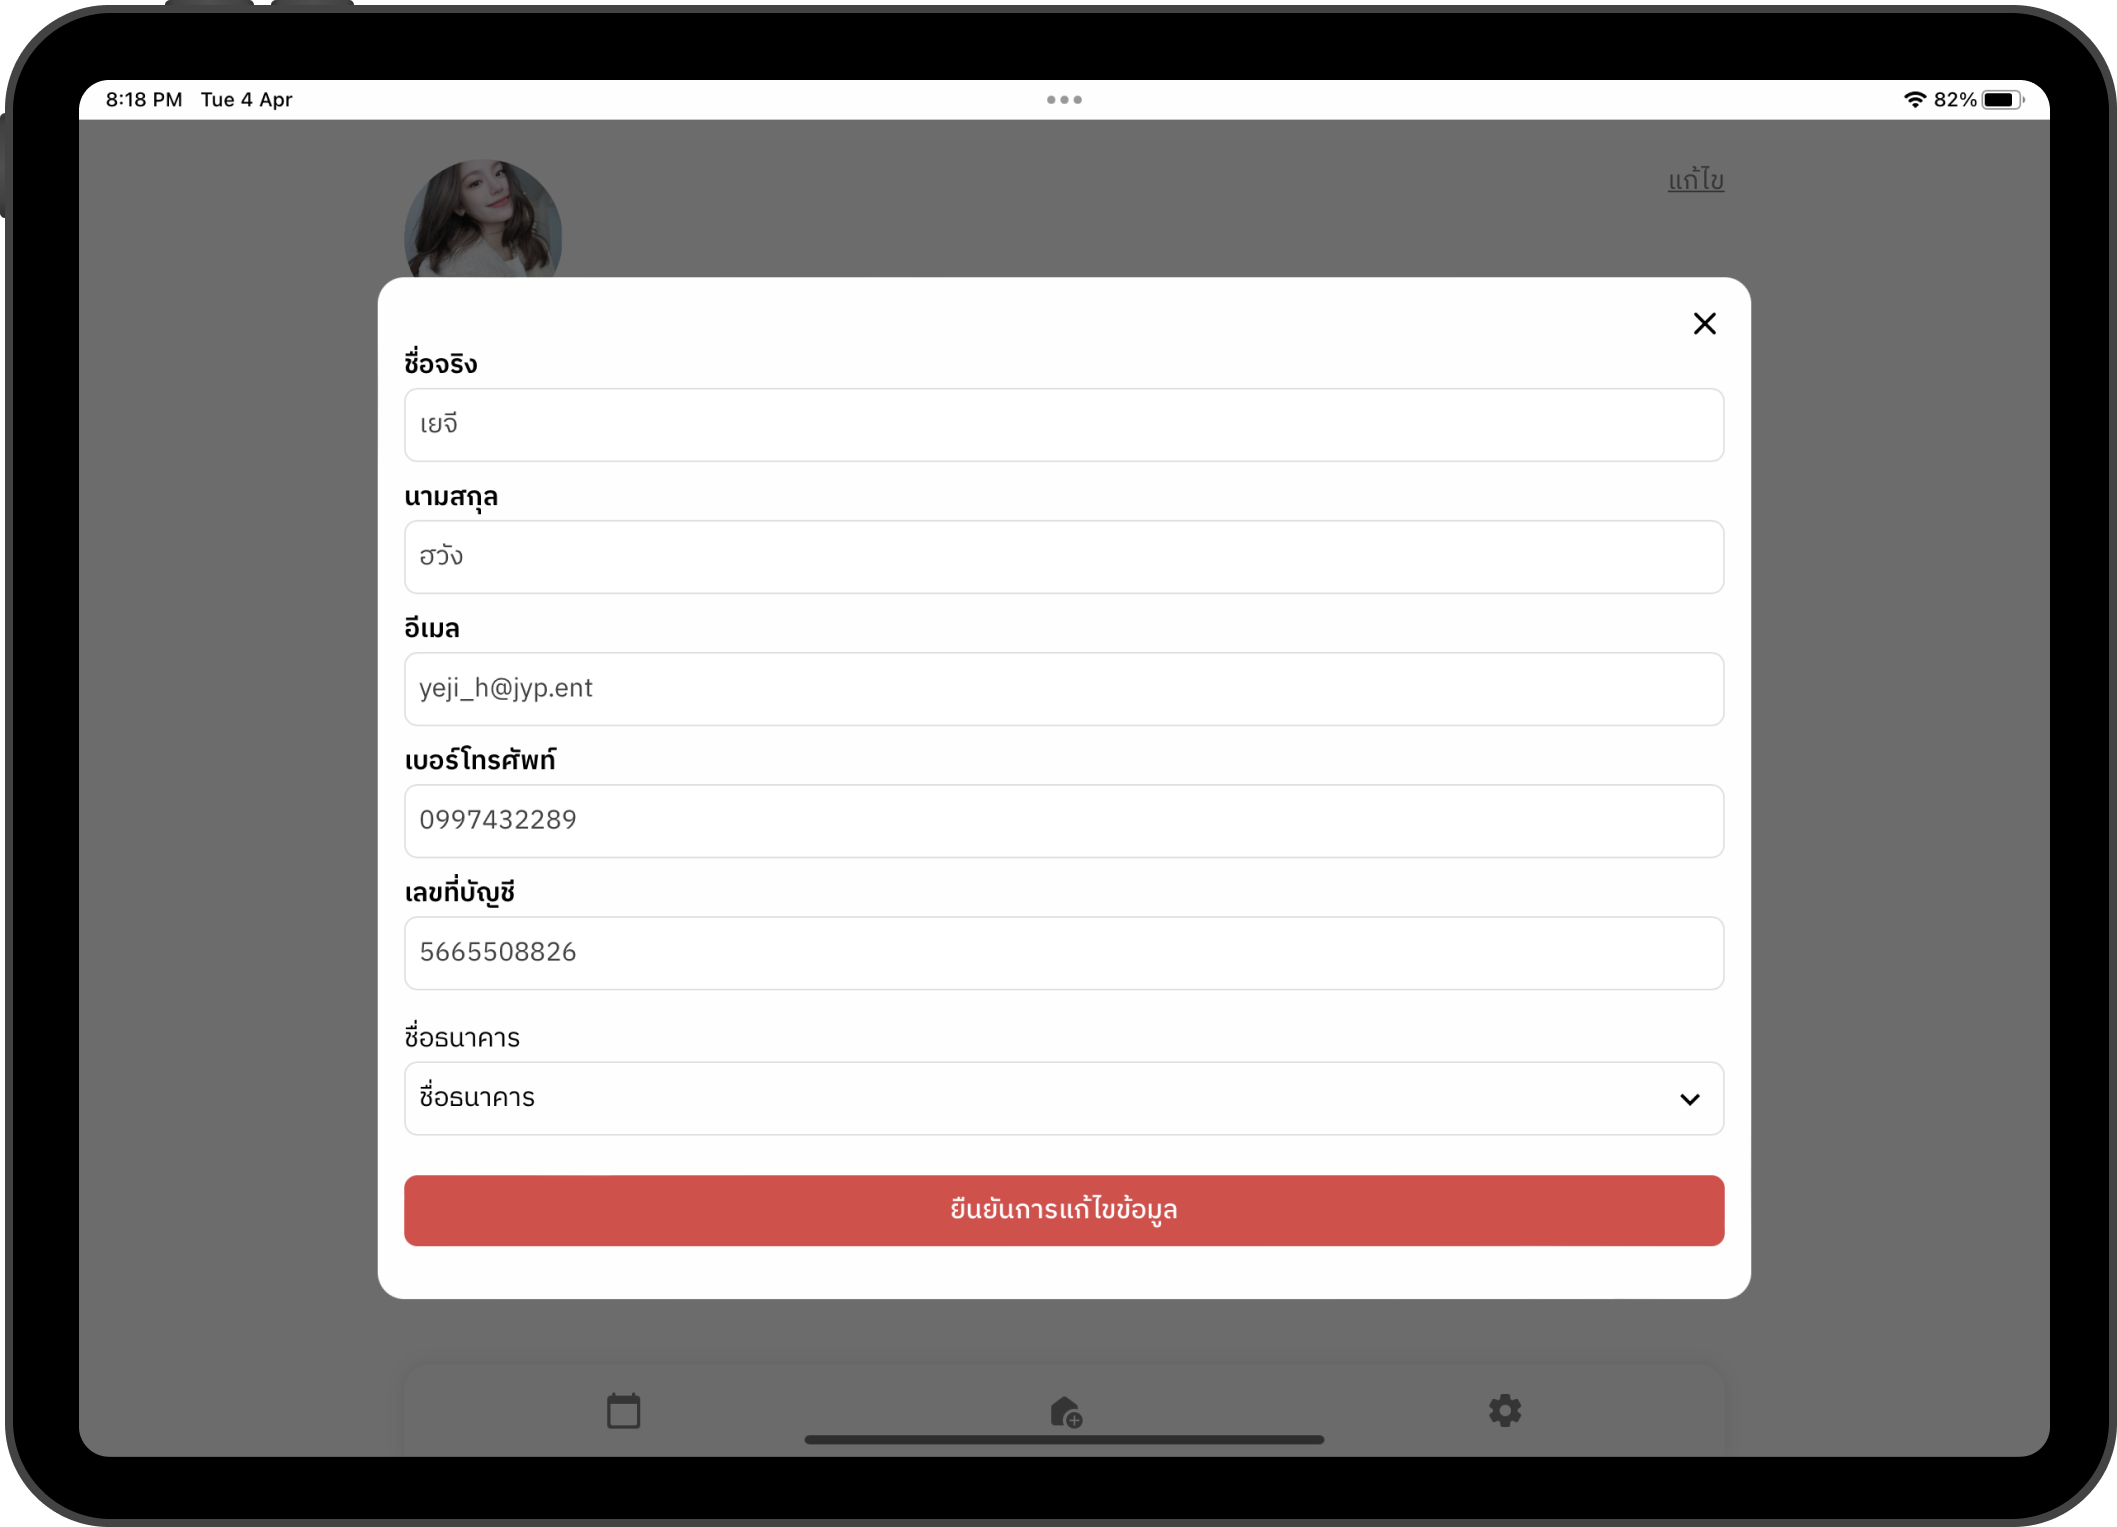
\includegraphics[width=5.5in]{./image/Flowider_edit_account.png}
    \end{center}
    \caption[Flowider edit account]{หน้าแก้ไขข้อมูลส่วนตัวของผู้ให้บริการ}
    \label{fig:Flowider_edit_account}
\end{figure}
\begin{figure}[ht]
    \begin{center}
    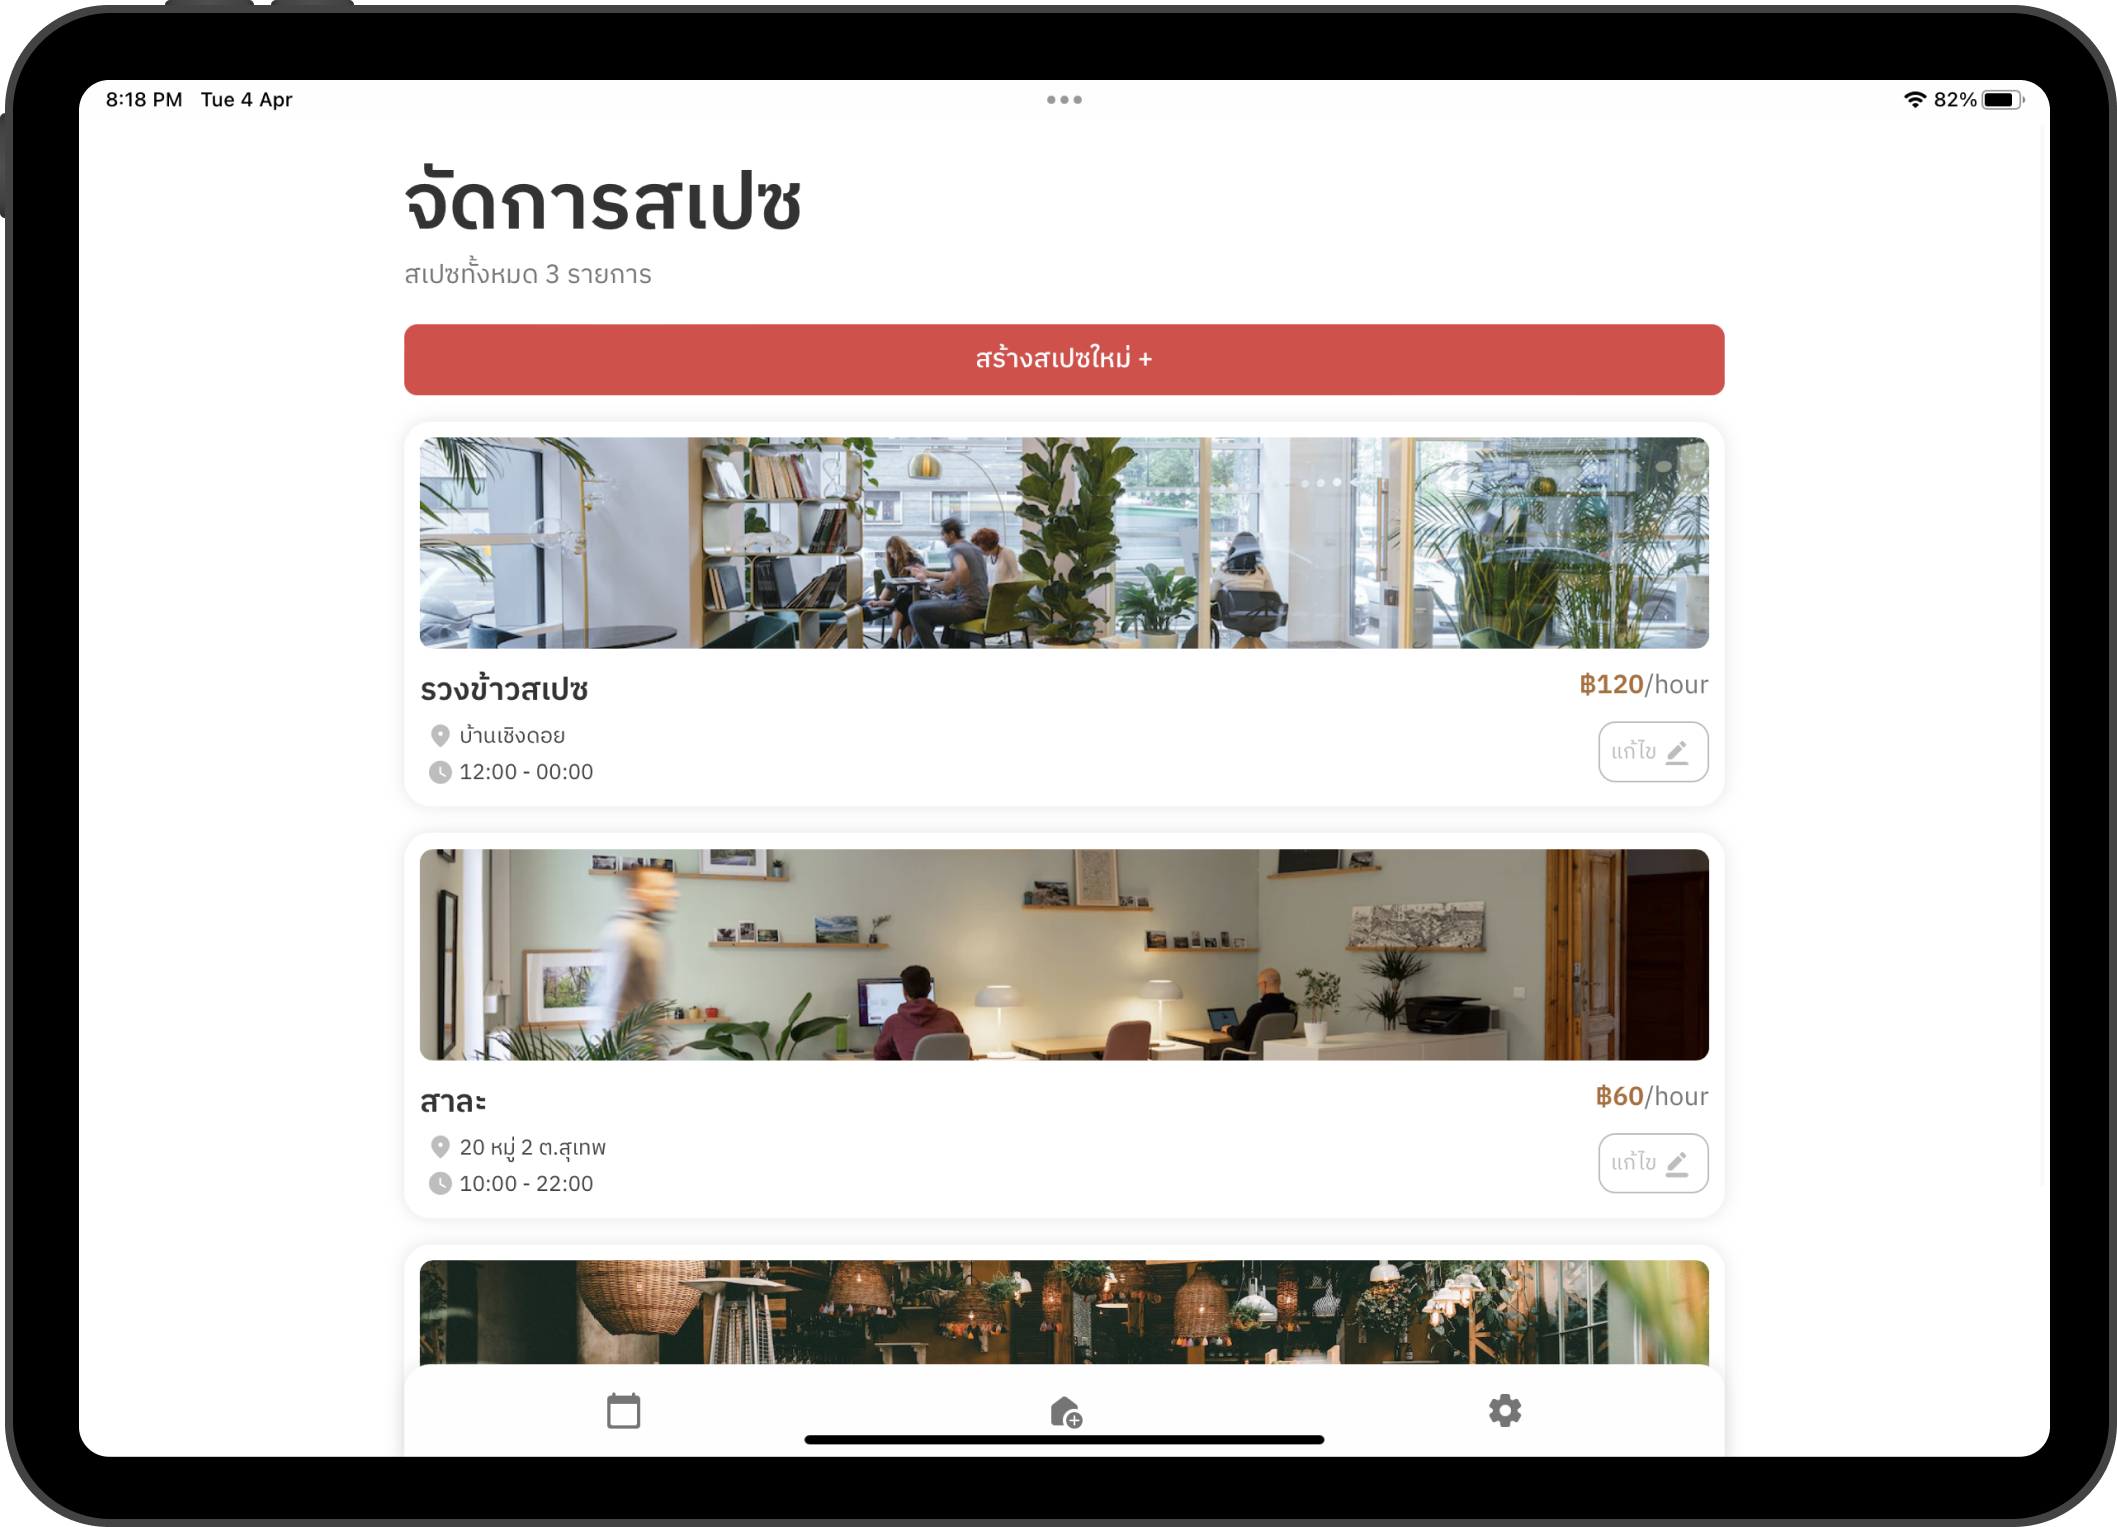
\includegraphics[width=5.5in]{./image/Flowider_space_mgmt.png}
    \end{center}
    \caption[Flowider space management]{หน้าจัดการสเปซ}
    \label{fig:Flowider_space_mgmt}
\end{figure}
\begin{figure}[ht]
    \begin{center}
    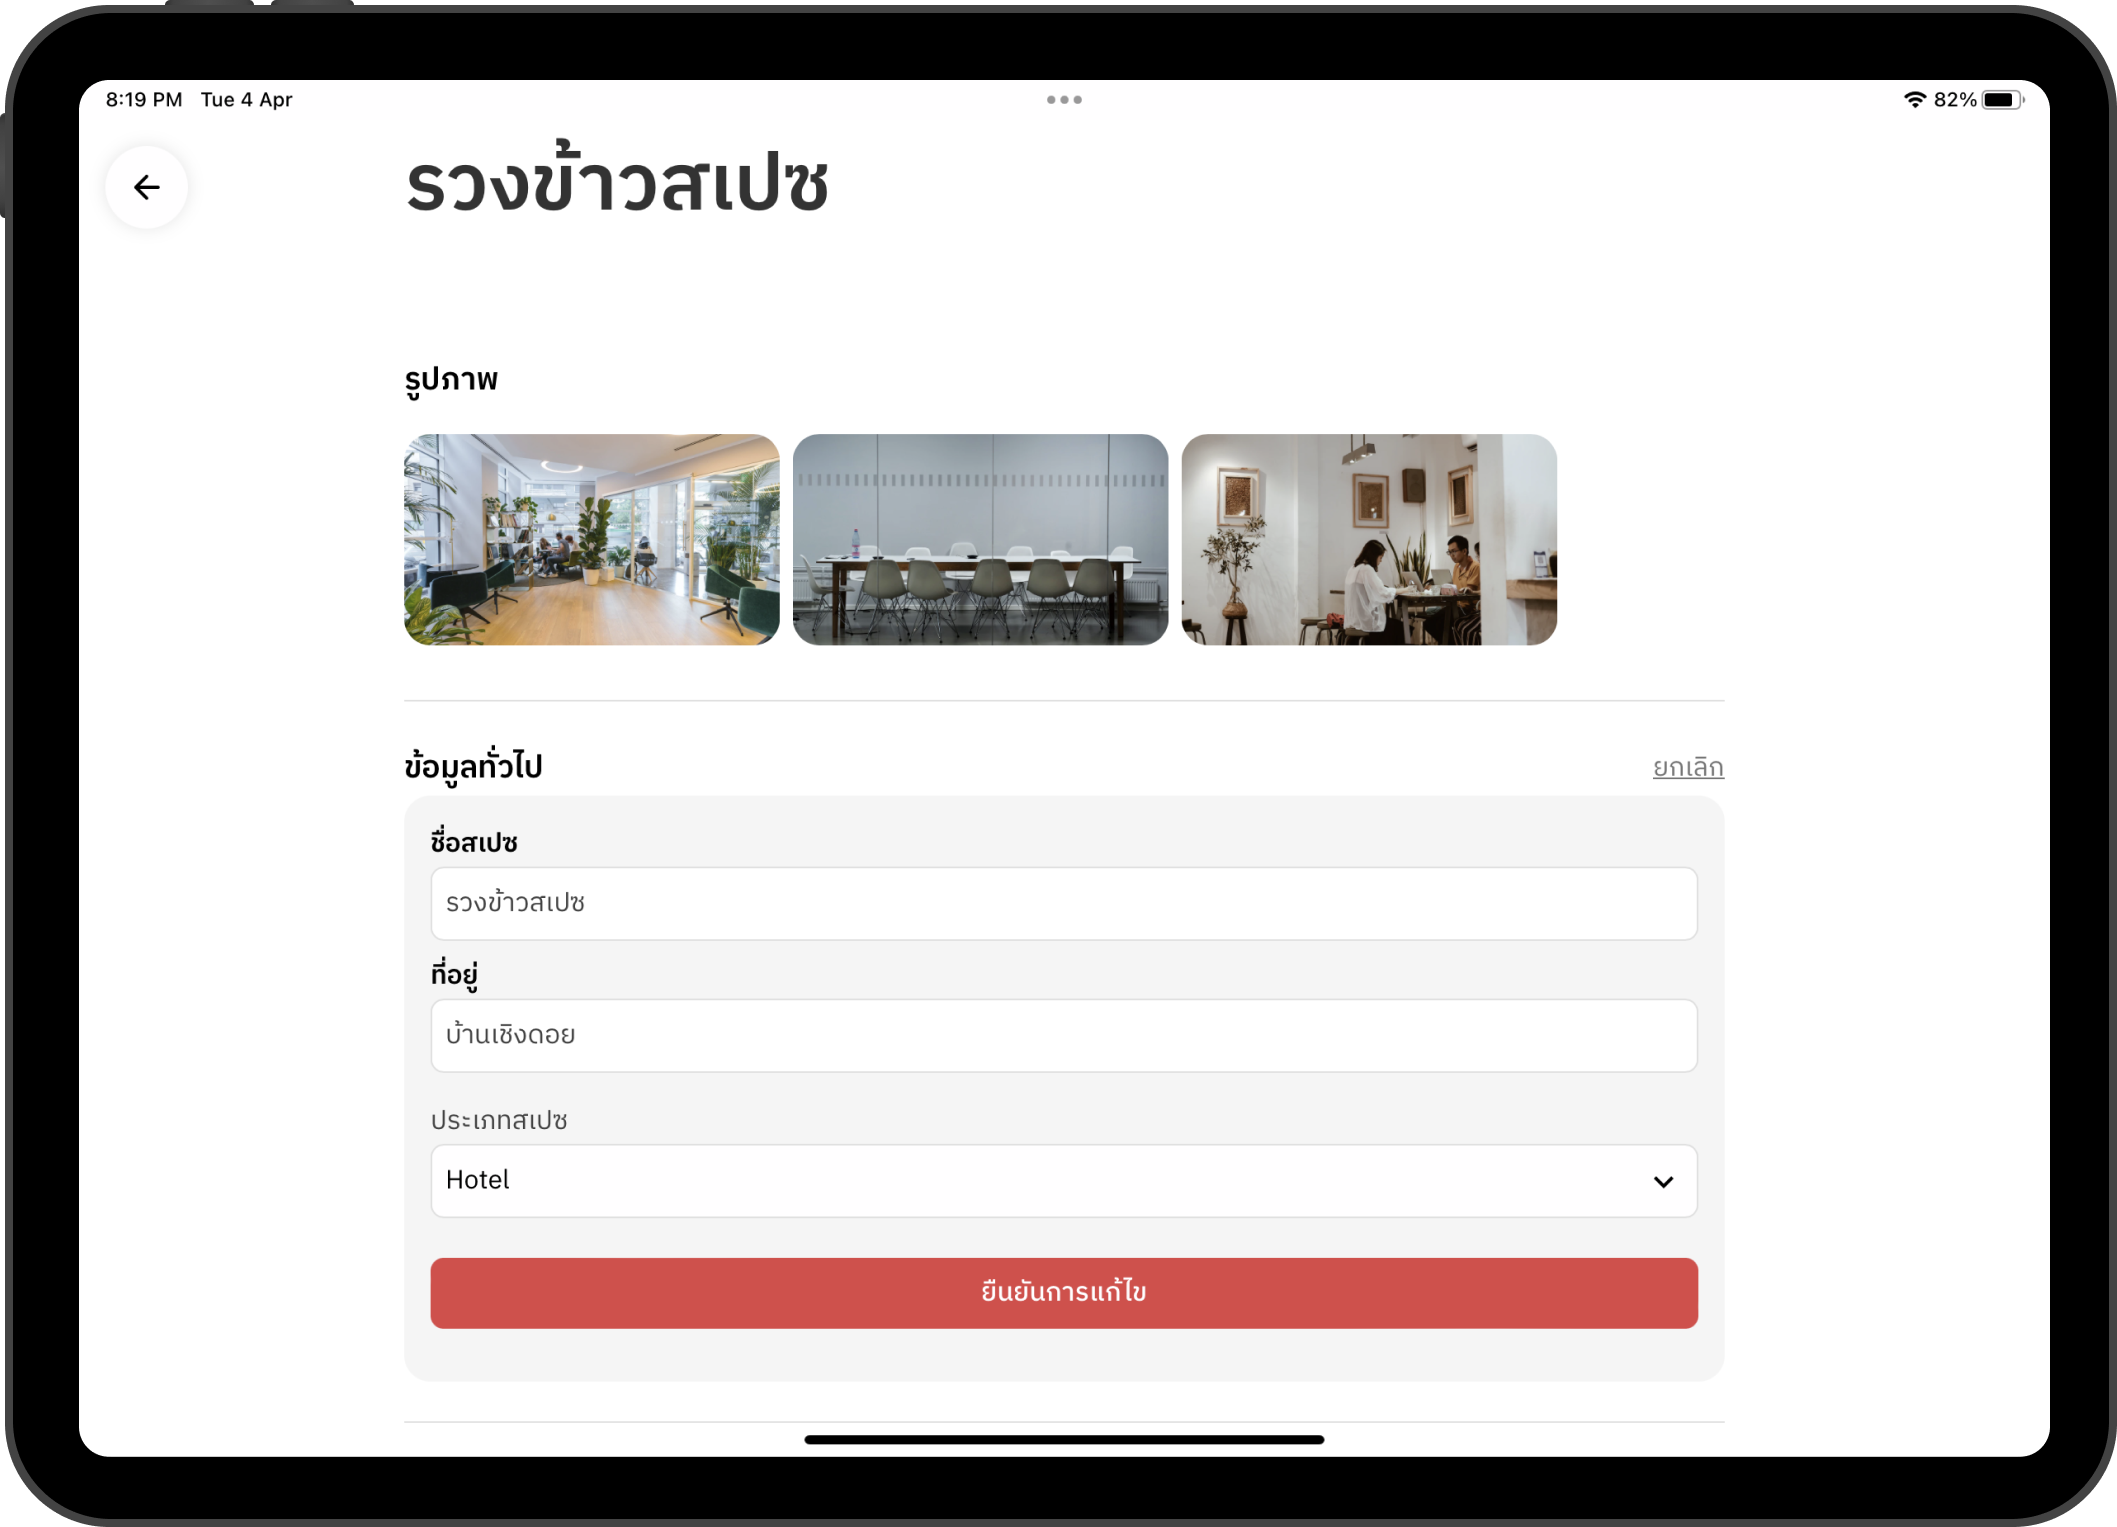
\includegraphics[width=5.5in]{./image/Flowider_space_edit_1.png}
    \end{center}
    \caption[Flowider space edit 1]{หน้าแก้ไขข้อมูลของสเปซ}
    \label{fig:Flowider_space_edit_1}
\end{figure}
\begin{figure}[ht]
    \begin{center}
    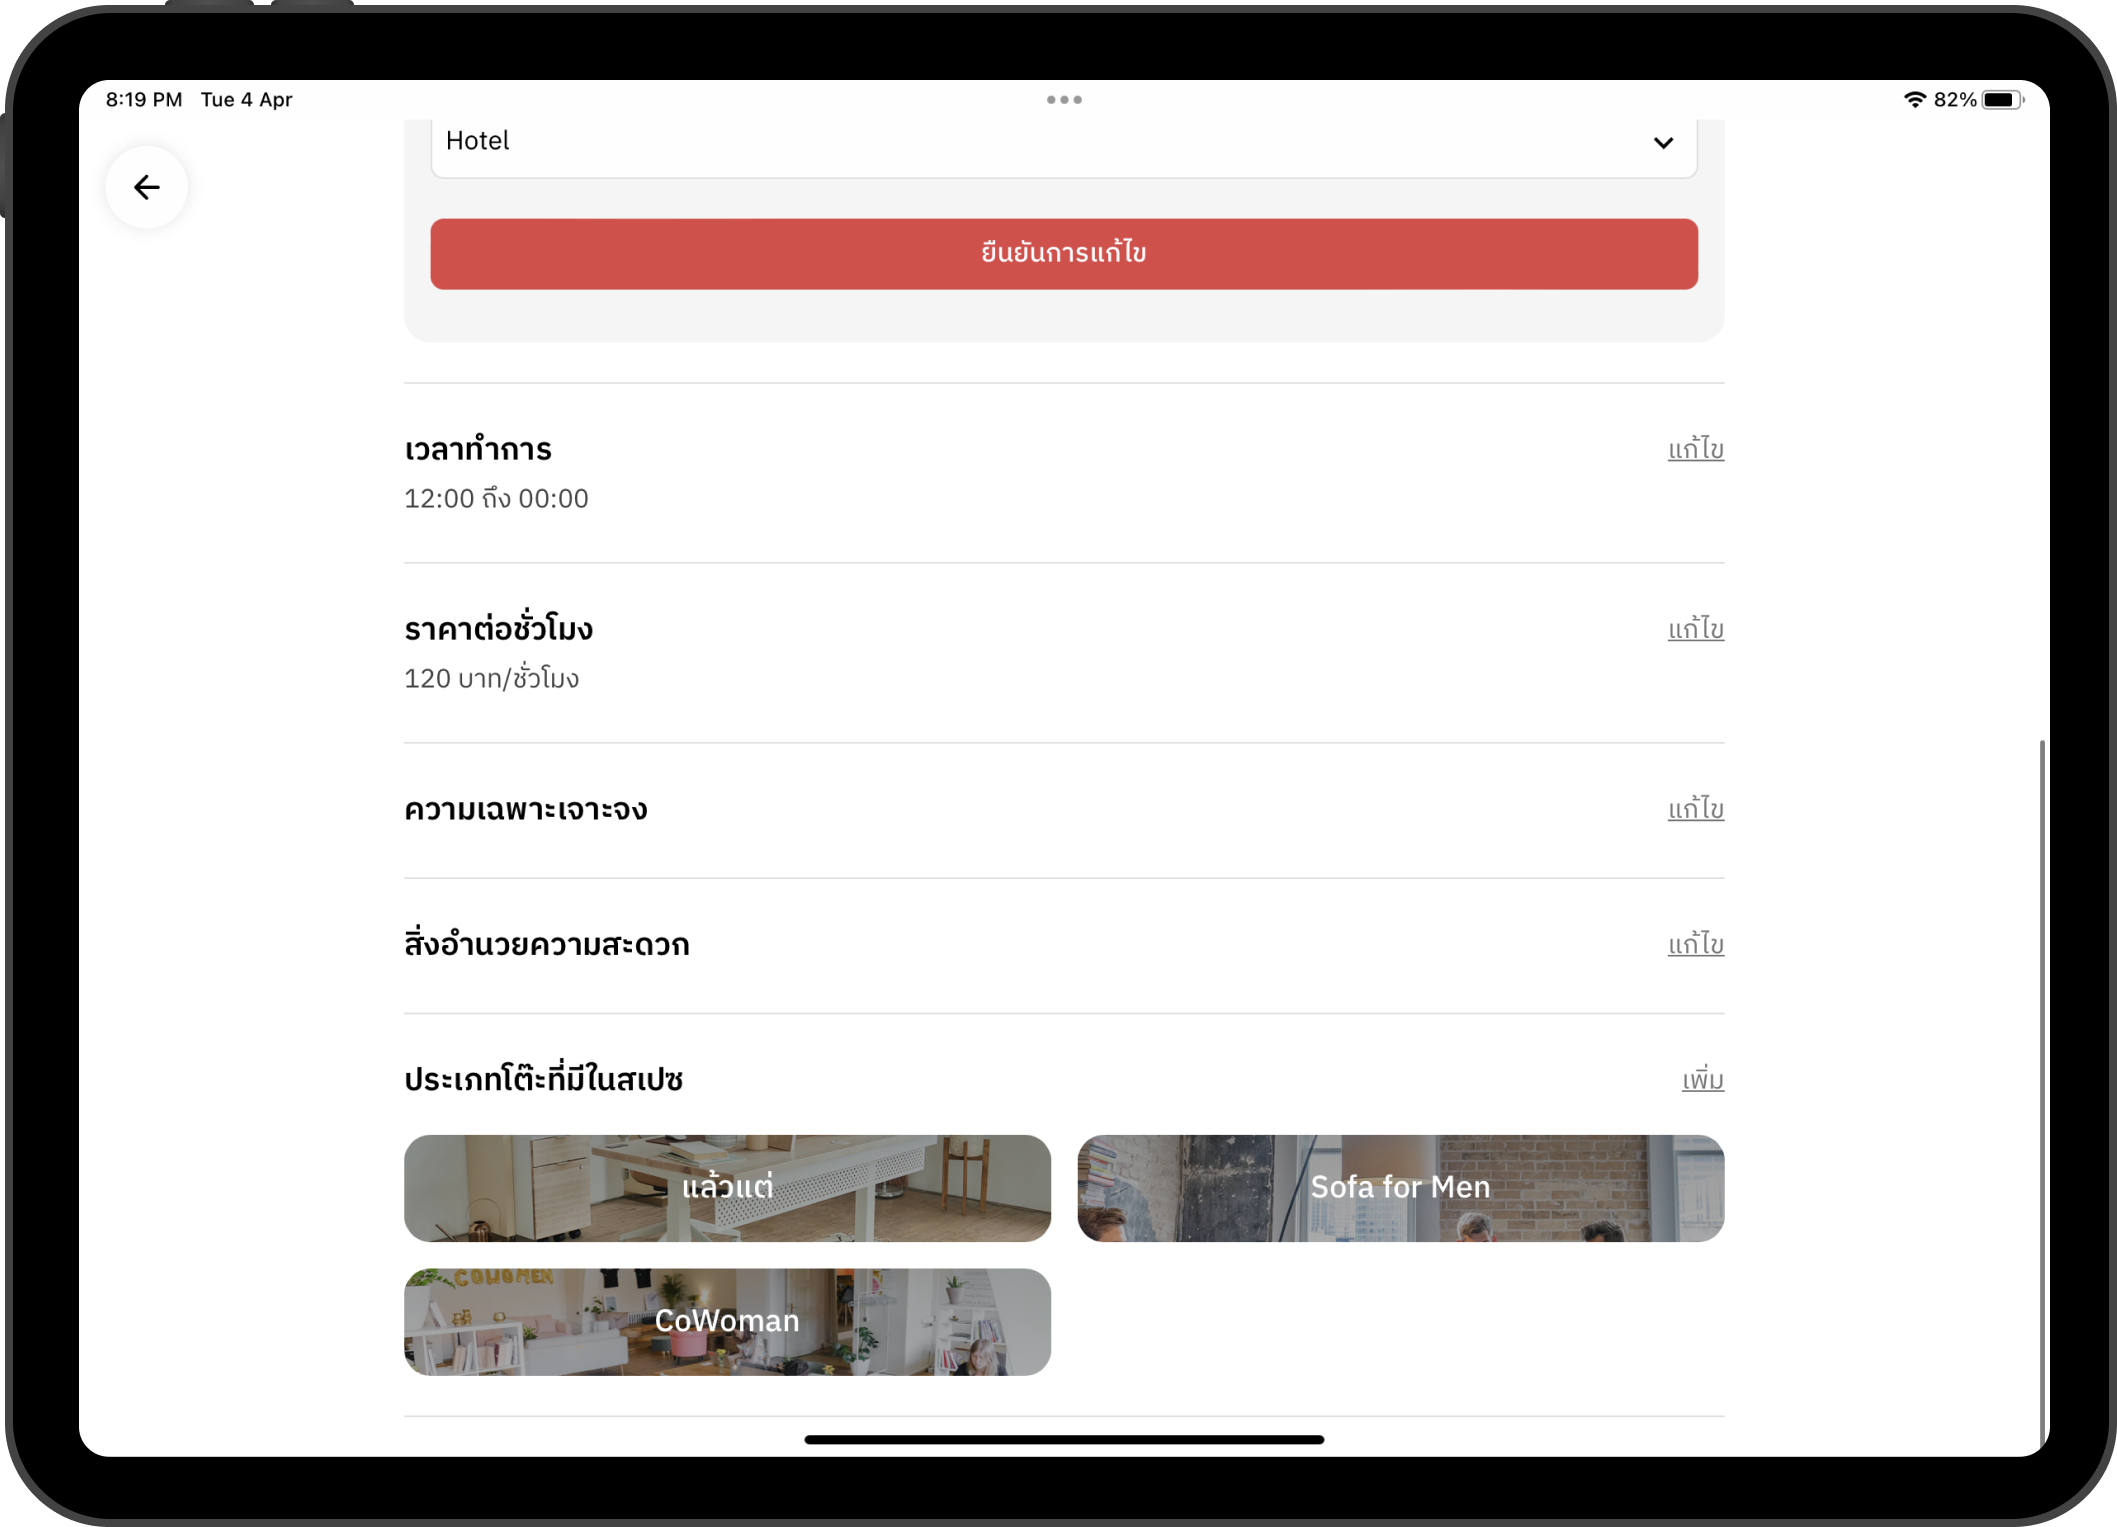
\includegraphics[width=5.5in]{./image/Flowider_space_edit_2.png}
    \end{center}
    \caption[Flowider space edit 2]{หน้าแก้ไขข้อมูลของสเปซ (ต่อ)}
    \label{fig:Flowider_space_edit_2}
\end{figure}
\begin{figure}[ht]
    \begin{center}
    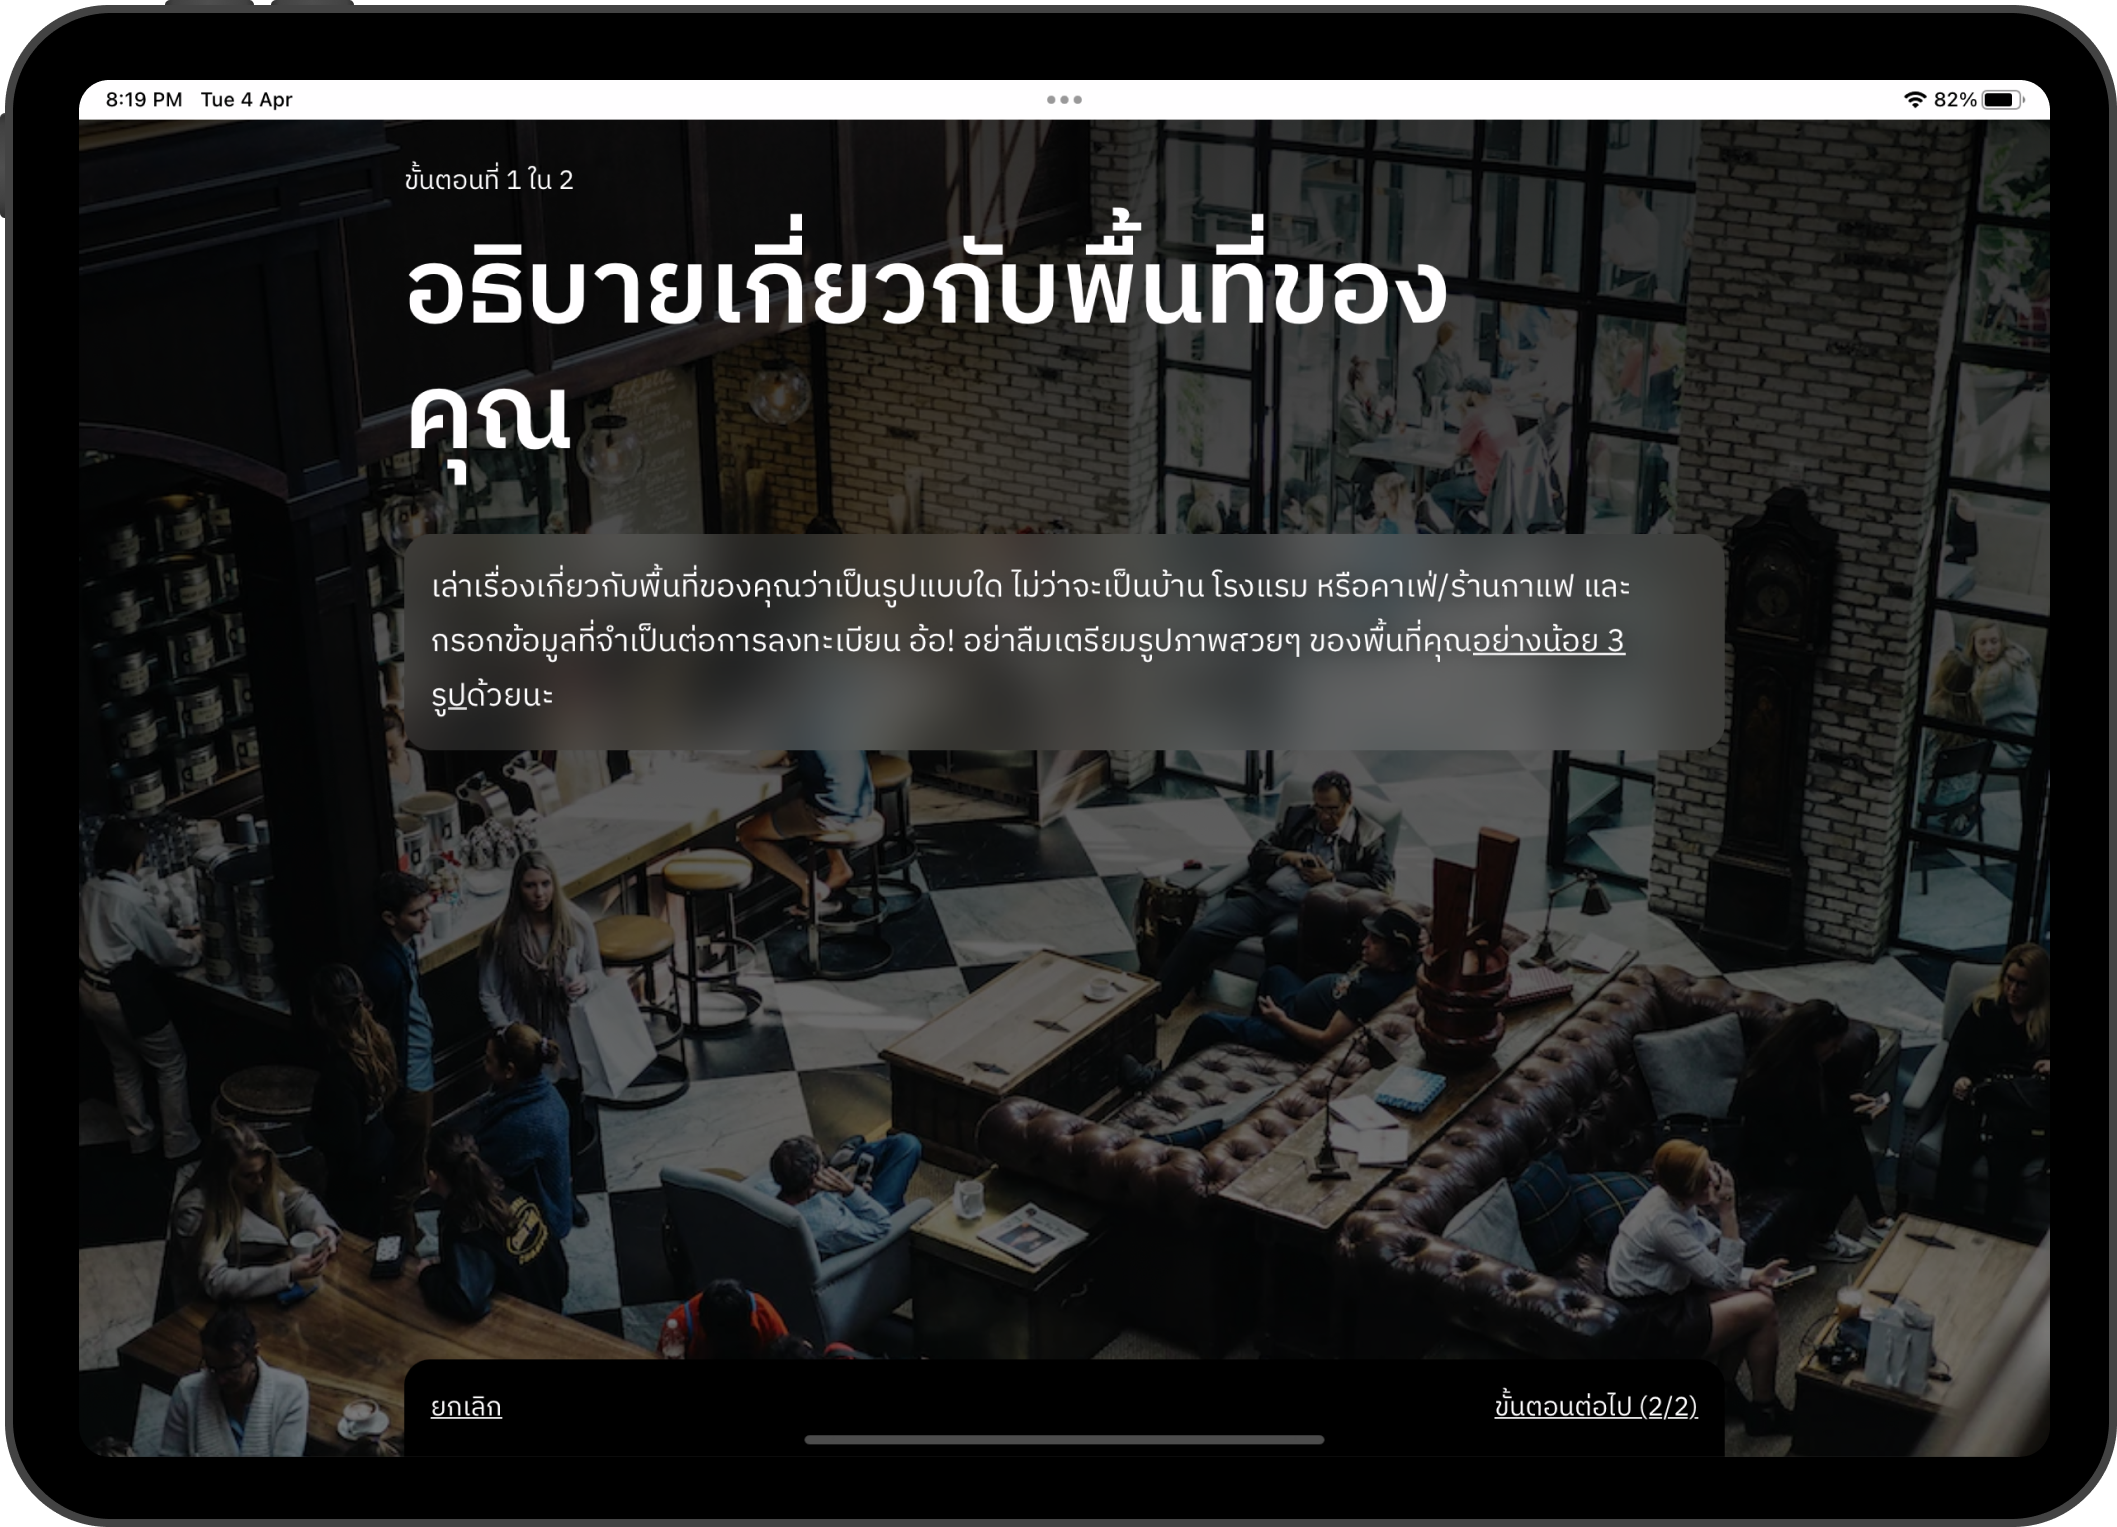
\includegraphics[width=5.5in]{./image/Flowider_onboarding_1.png}
    \end{center}
    \caption[Flowider onboarding 1]{หน้าเตรียมข้อมูลของสเปซก่อนทำการลงทะเบียน}
    \label{fig:Flowider_onboarding_1}
\end{figure}
\begin{figure}[ht]
    \begin{center}
    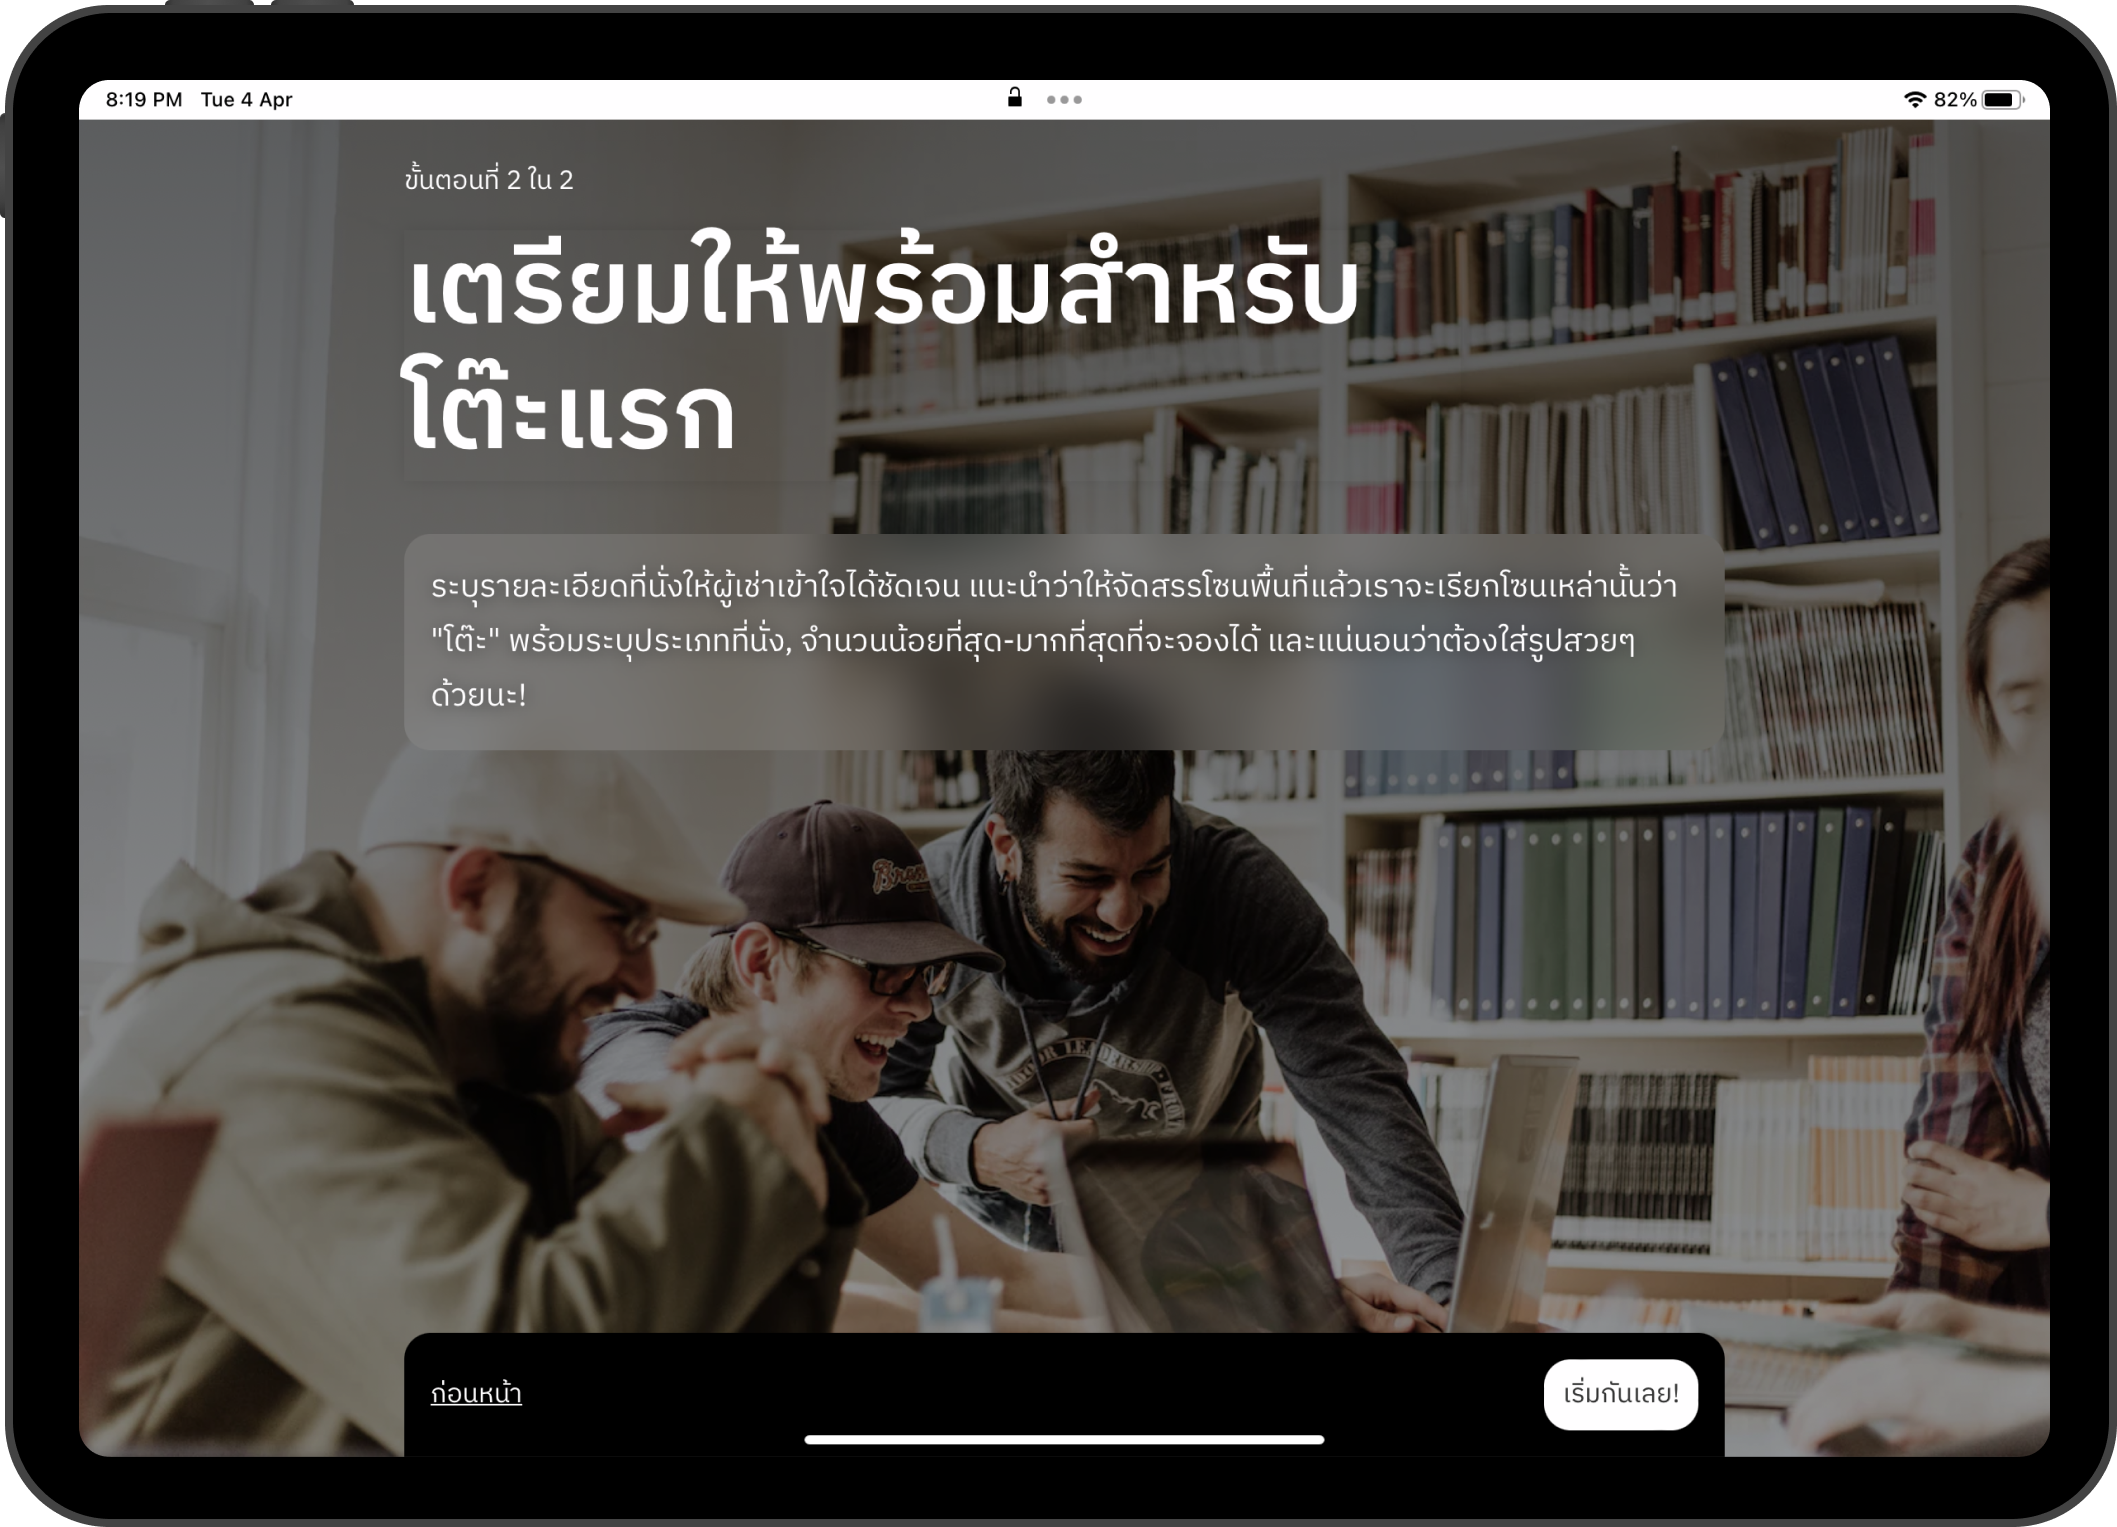
\includegraphics[width=5.5in]{./image/Flowider_onboarding_2.png}
    \end{center}
    \caption[Flowider onboarding 2]{หน้าเตรียมข้อมูลของโต๊ะก่อนทำการลงทะเบียน}
    \label{fig:Flowider_onboarding_2}
\end{figure}
\begin{figure}[ht]
    \begin{center}
    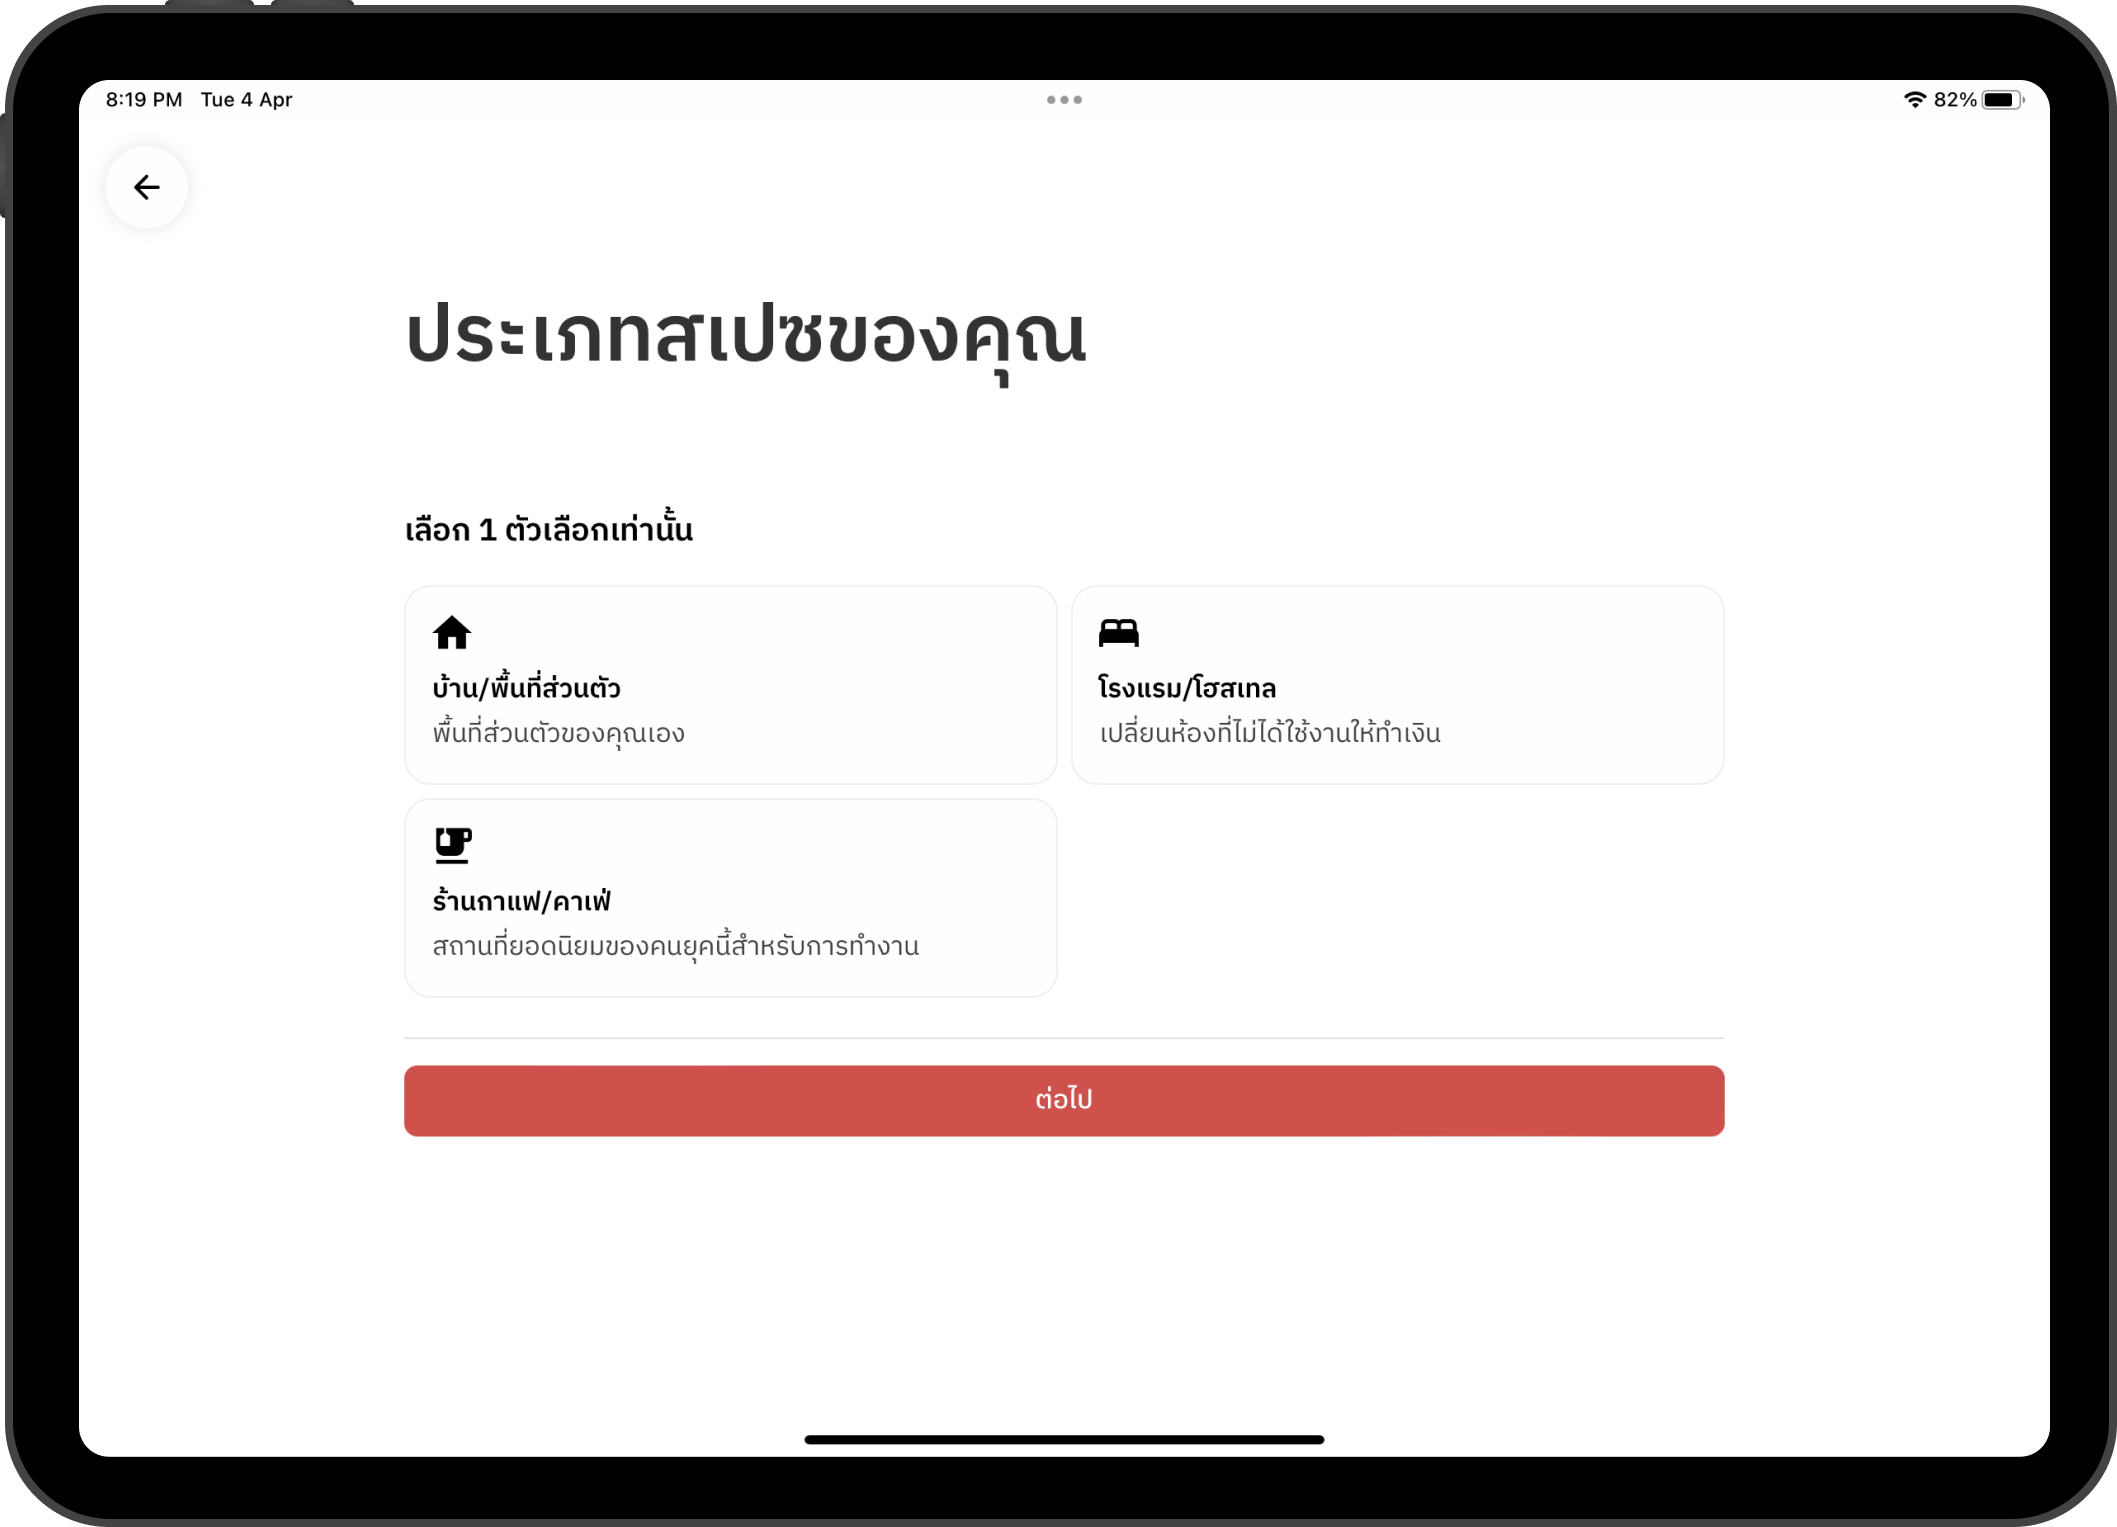
\includegraphics[width=5.5in]{./image/Flowider_place_category.png}
    \end{center}
    \caption[Flowider place category]{หน้าระบุประเภทของสเปซ}
    \label{fig:Flowider_place_category}
\end{figure}
\begin{figure}[ht]
    \begin{center}
    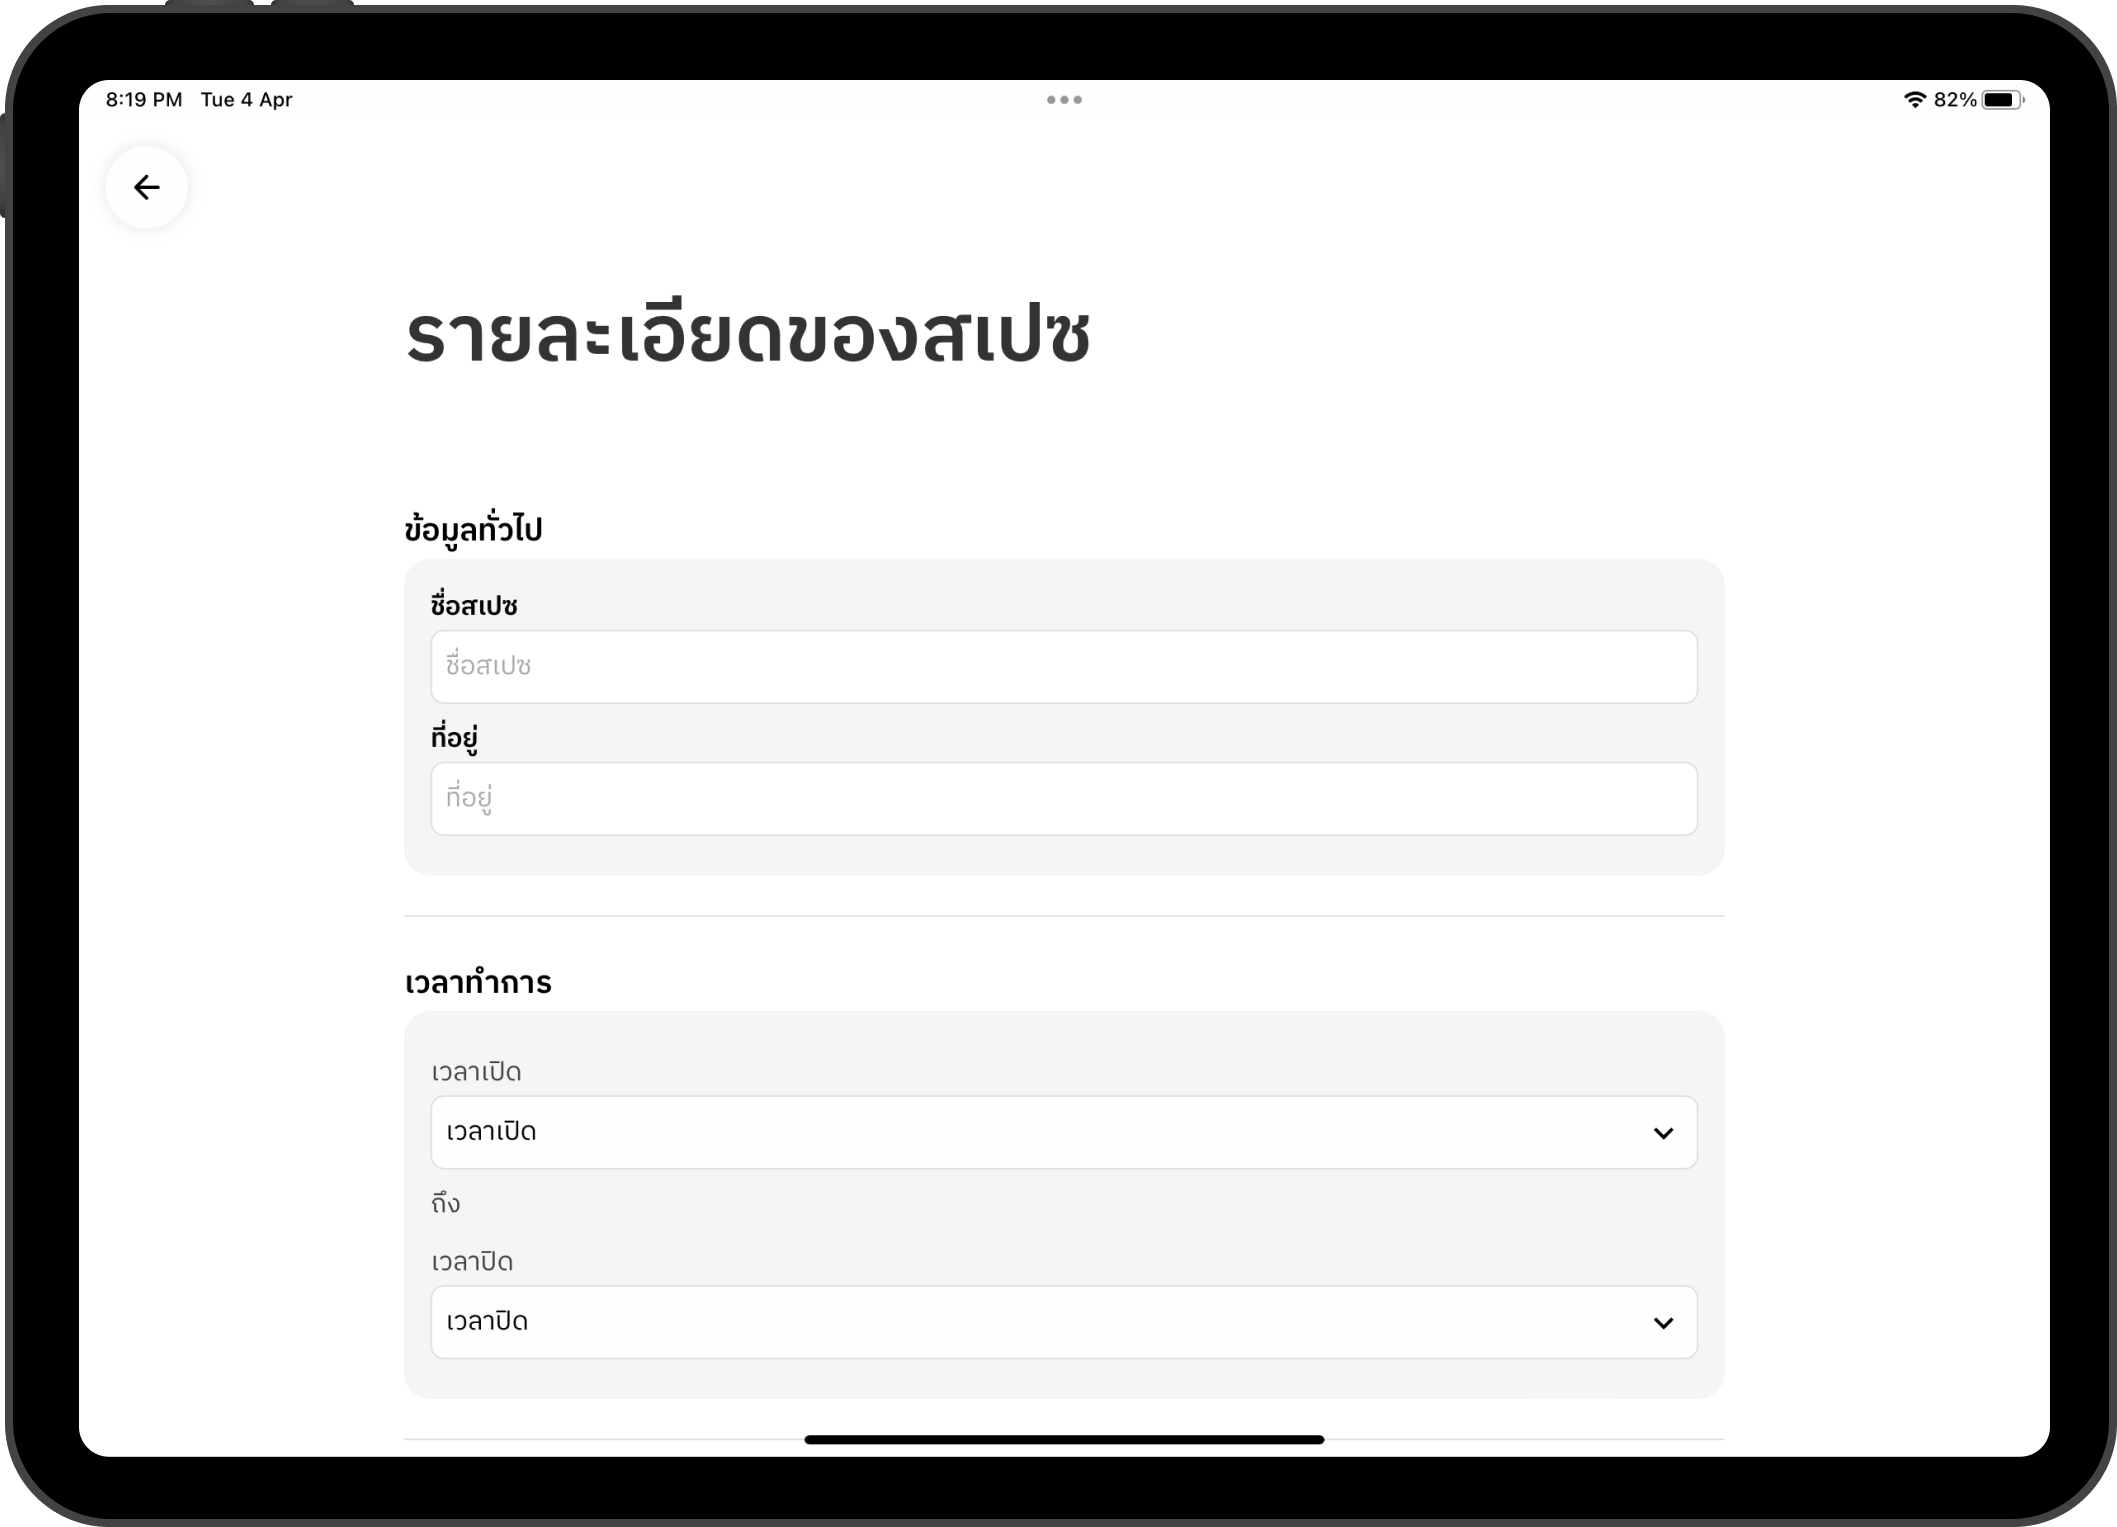
\includegraphics[width=5.5in]{./image/Flowider_place_info_1.png}
    \end{center}
    \caption[Flowider place info 1]{หน้าระบุรายละเอียดของสเปซ}
    \label{fig:Flowider_place_info_1}
\end{figure}
\begin{figure}[ht]
    \begin{center}
    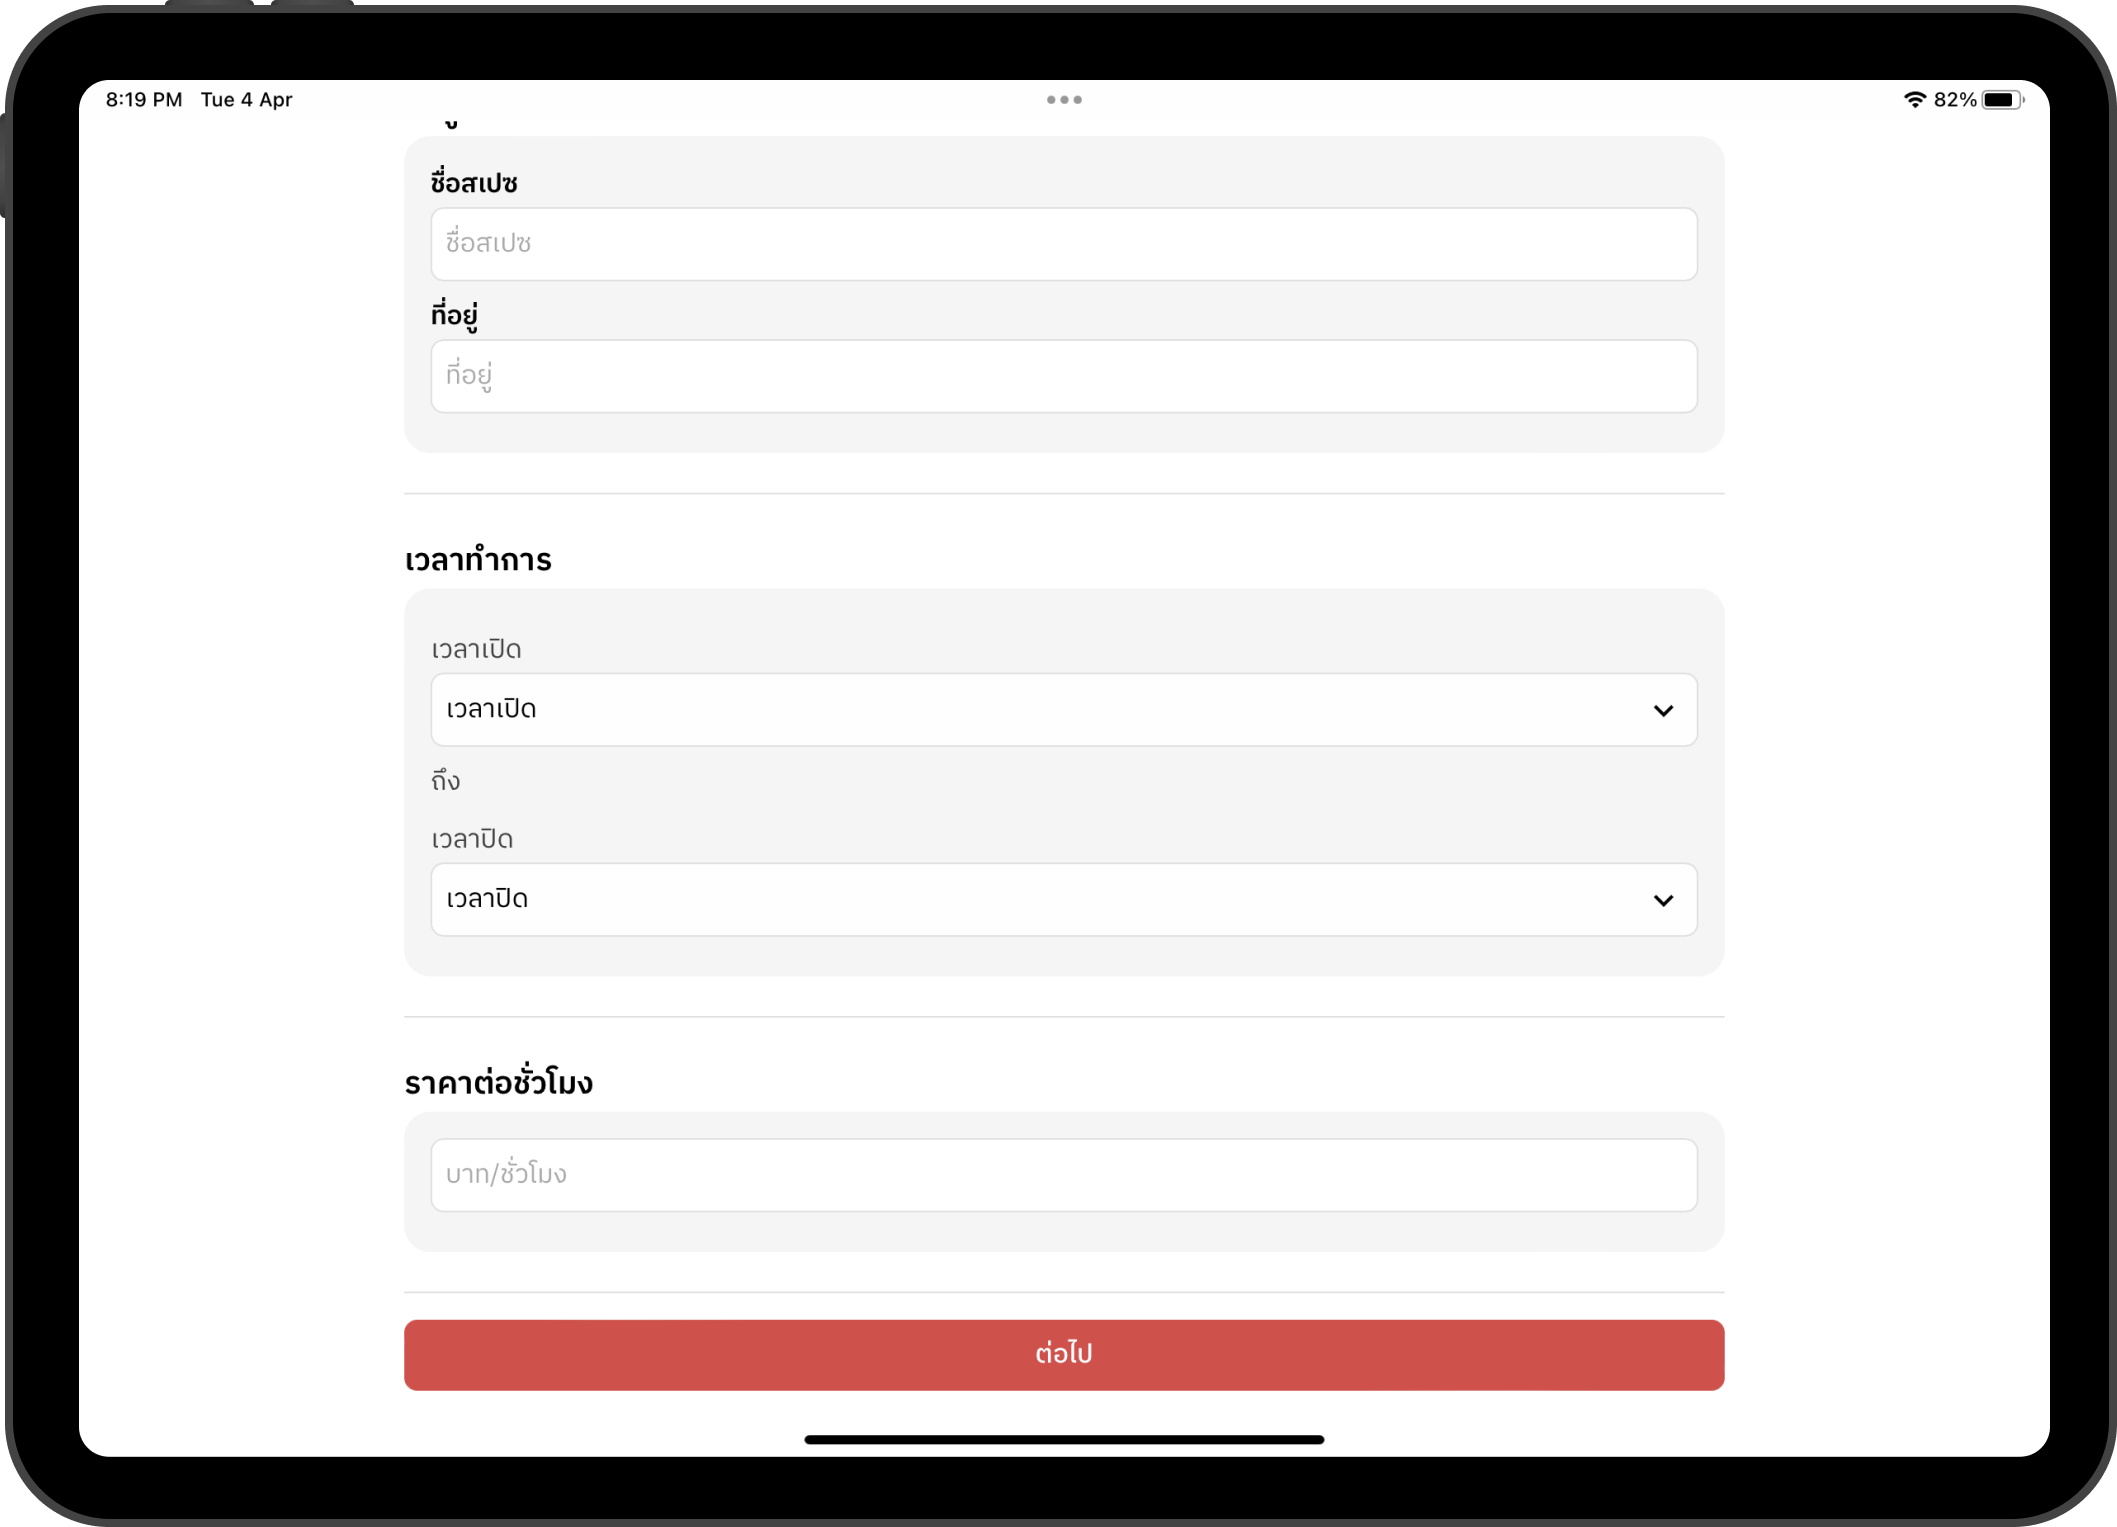
\includegraphics[width=5.5in]{./image/Flowider_place_info_2.png}
    \end{center}
    \caption[Flowider place info 2]{หน้าระบุรายละเอียดของสเปซ (ต่อ)}
    \label{fig:Flowider_place_info_2}
\end{figure}
\begin{figure}[ht]
    \begin{center}
    \includegraphics[width=5.5in]{./image/Flowider_place_Specification.png}
    \end{center}
    \caption[Flowider place Specification]{หน้าระบุความเฉาะเจาะจง}
    \label{fig:Flowider_place_Specification}
\end{figure}
\begin{figure}[ht]
    \begin{center}
    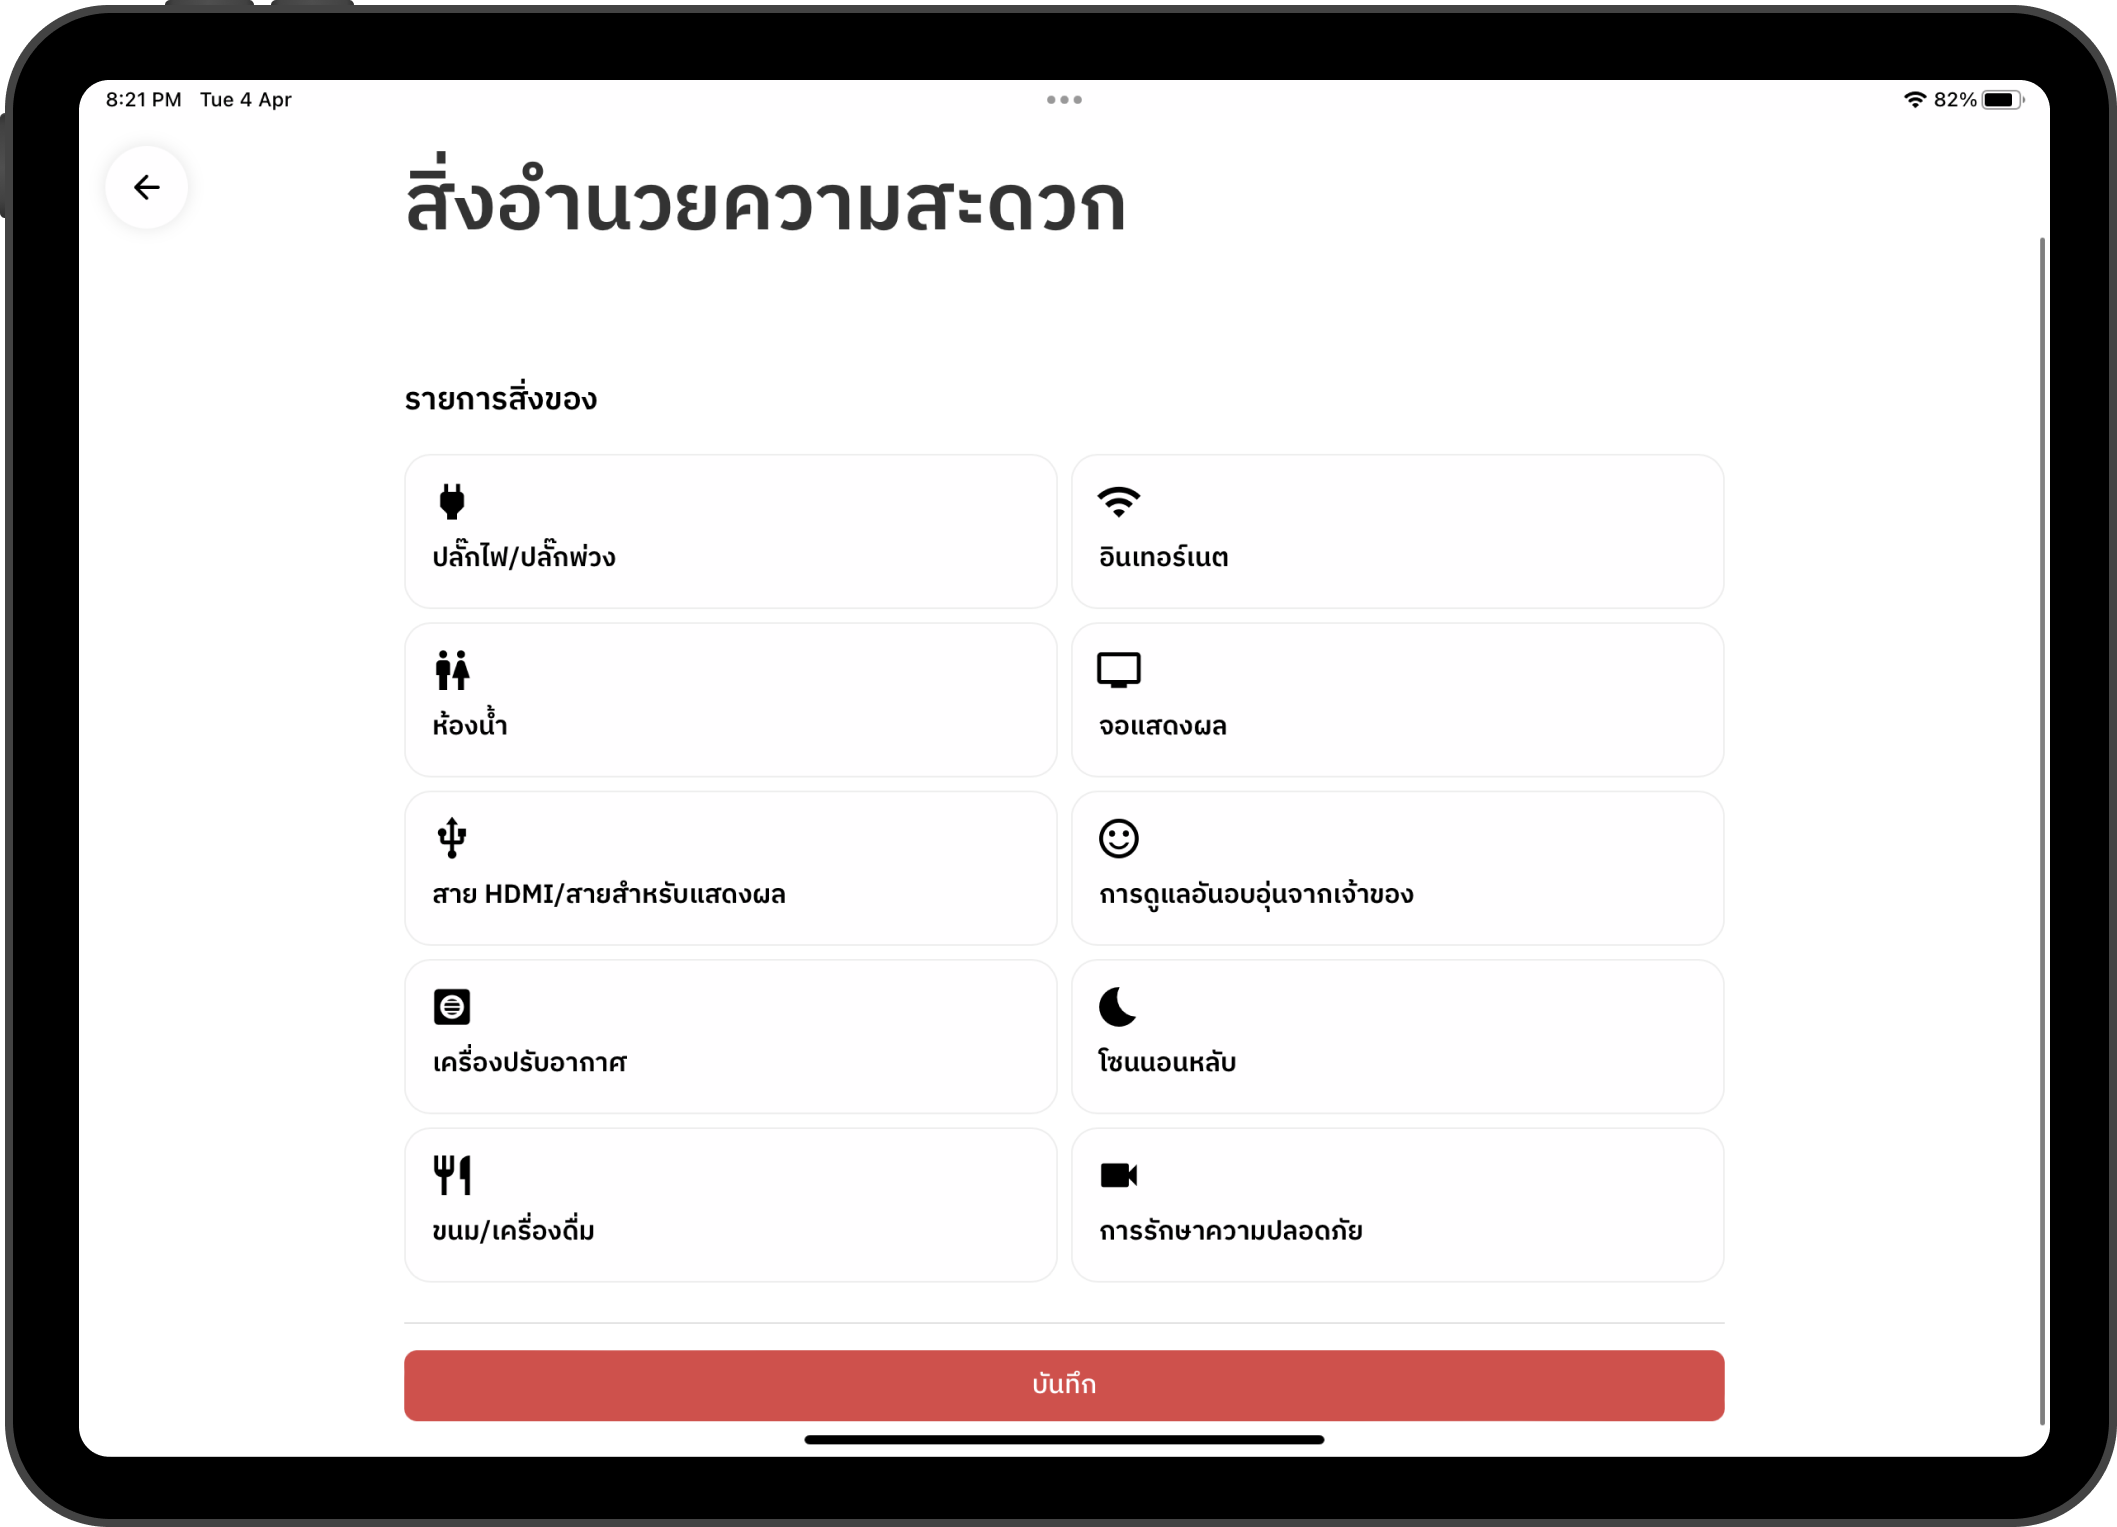
\includegraphics[width=5.5in]{./image/Flowider_place_amenity.png}
    \end{center}
    \caption[Flowider place amenity]{หน้าระบุสิ่งอำนวยความสะดวก}
    \label{fig:Flowider_place_amenity}
\end{figure}
\begin{figure}[ht]
    \begin{center}
    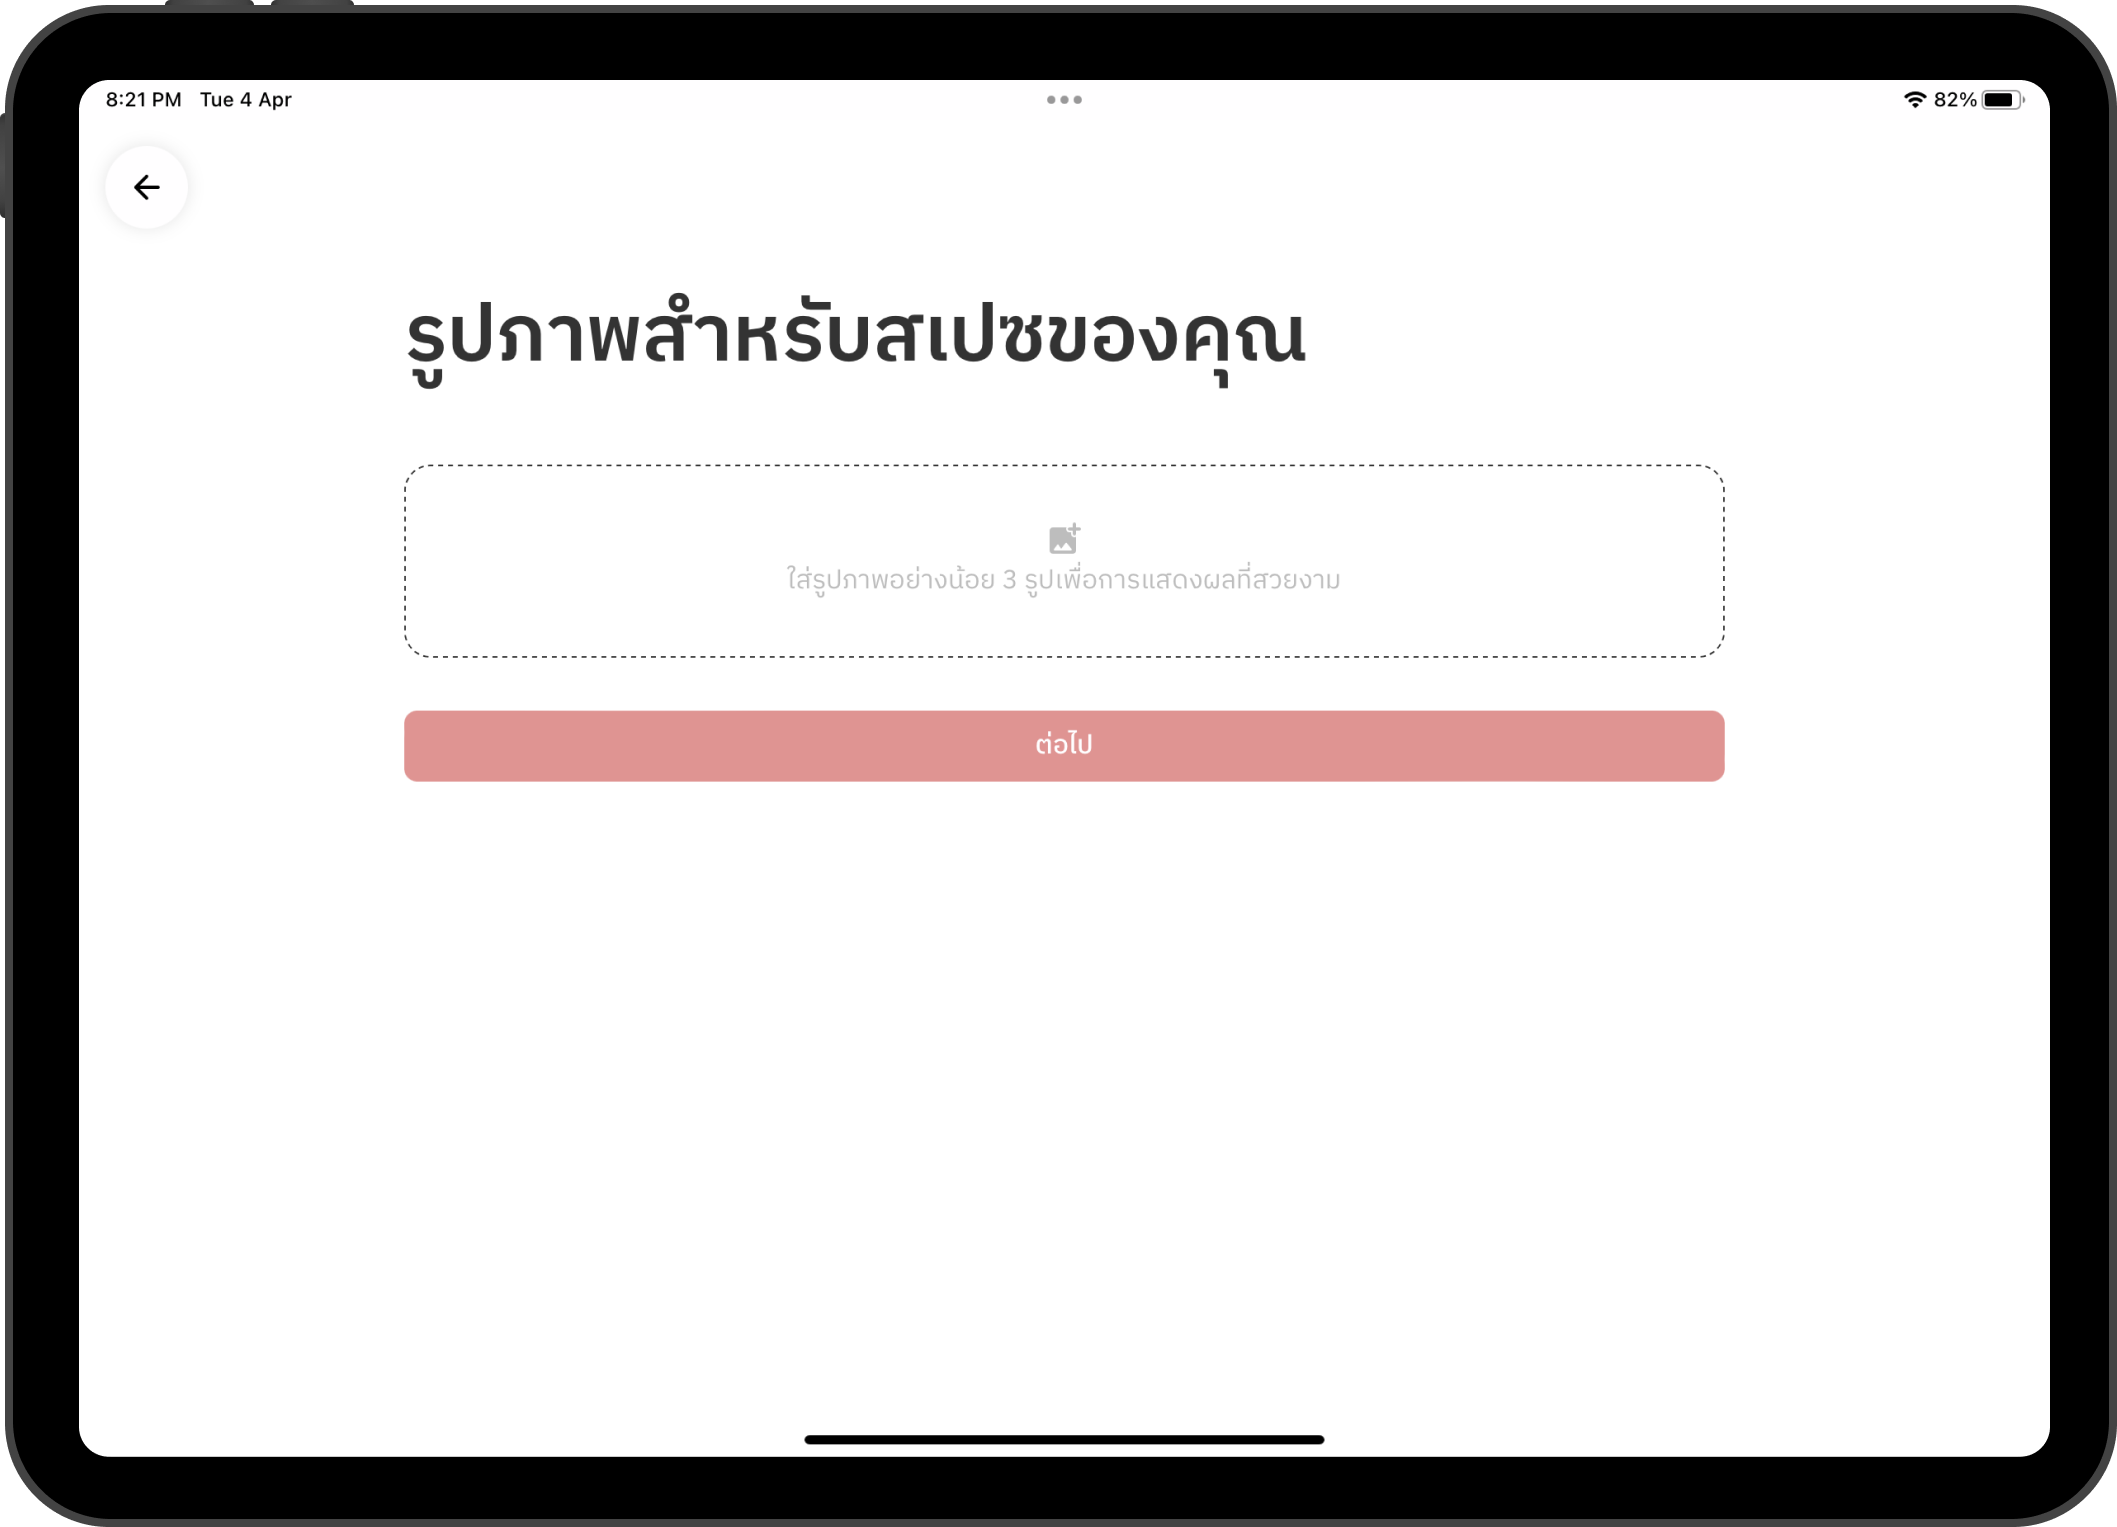
\includegraphics[width=5.5in]{./image/Flowider_place_img.png}
    \end{center}
    \caption[Flowider place image]{หน้าเพิ่มรูปภาพของสเปซ}
    \label{fig:Flowider_place_img}
\end{figure}
\begin{figure}[ht]
    \begin{center}
    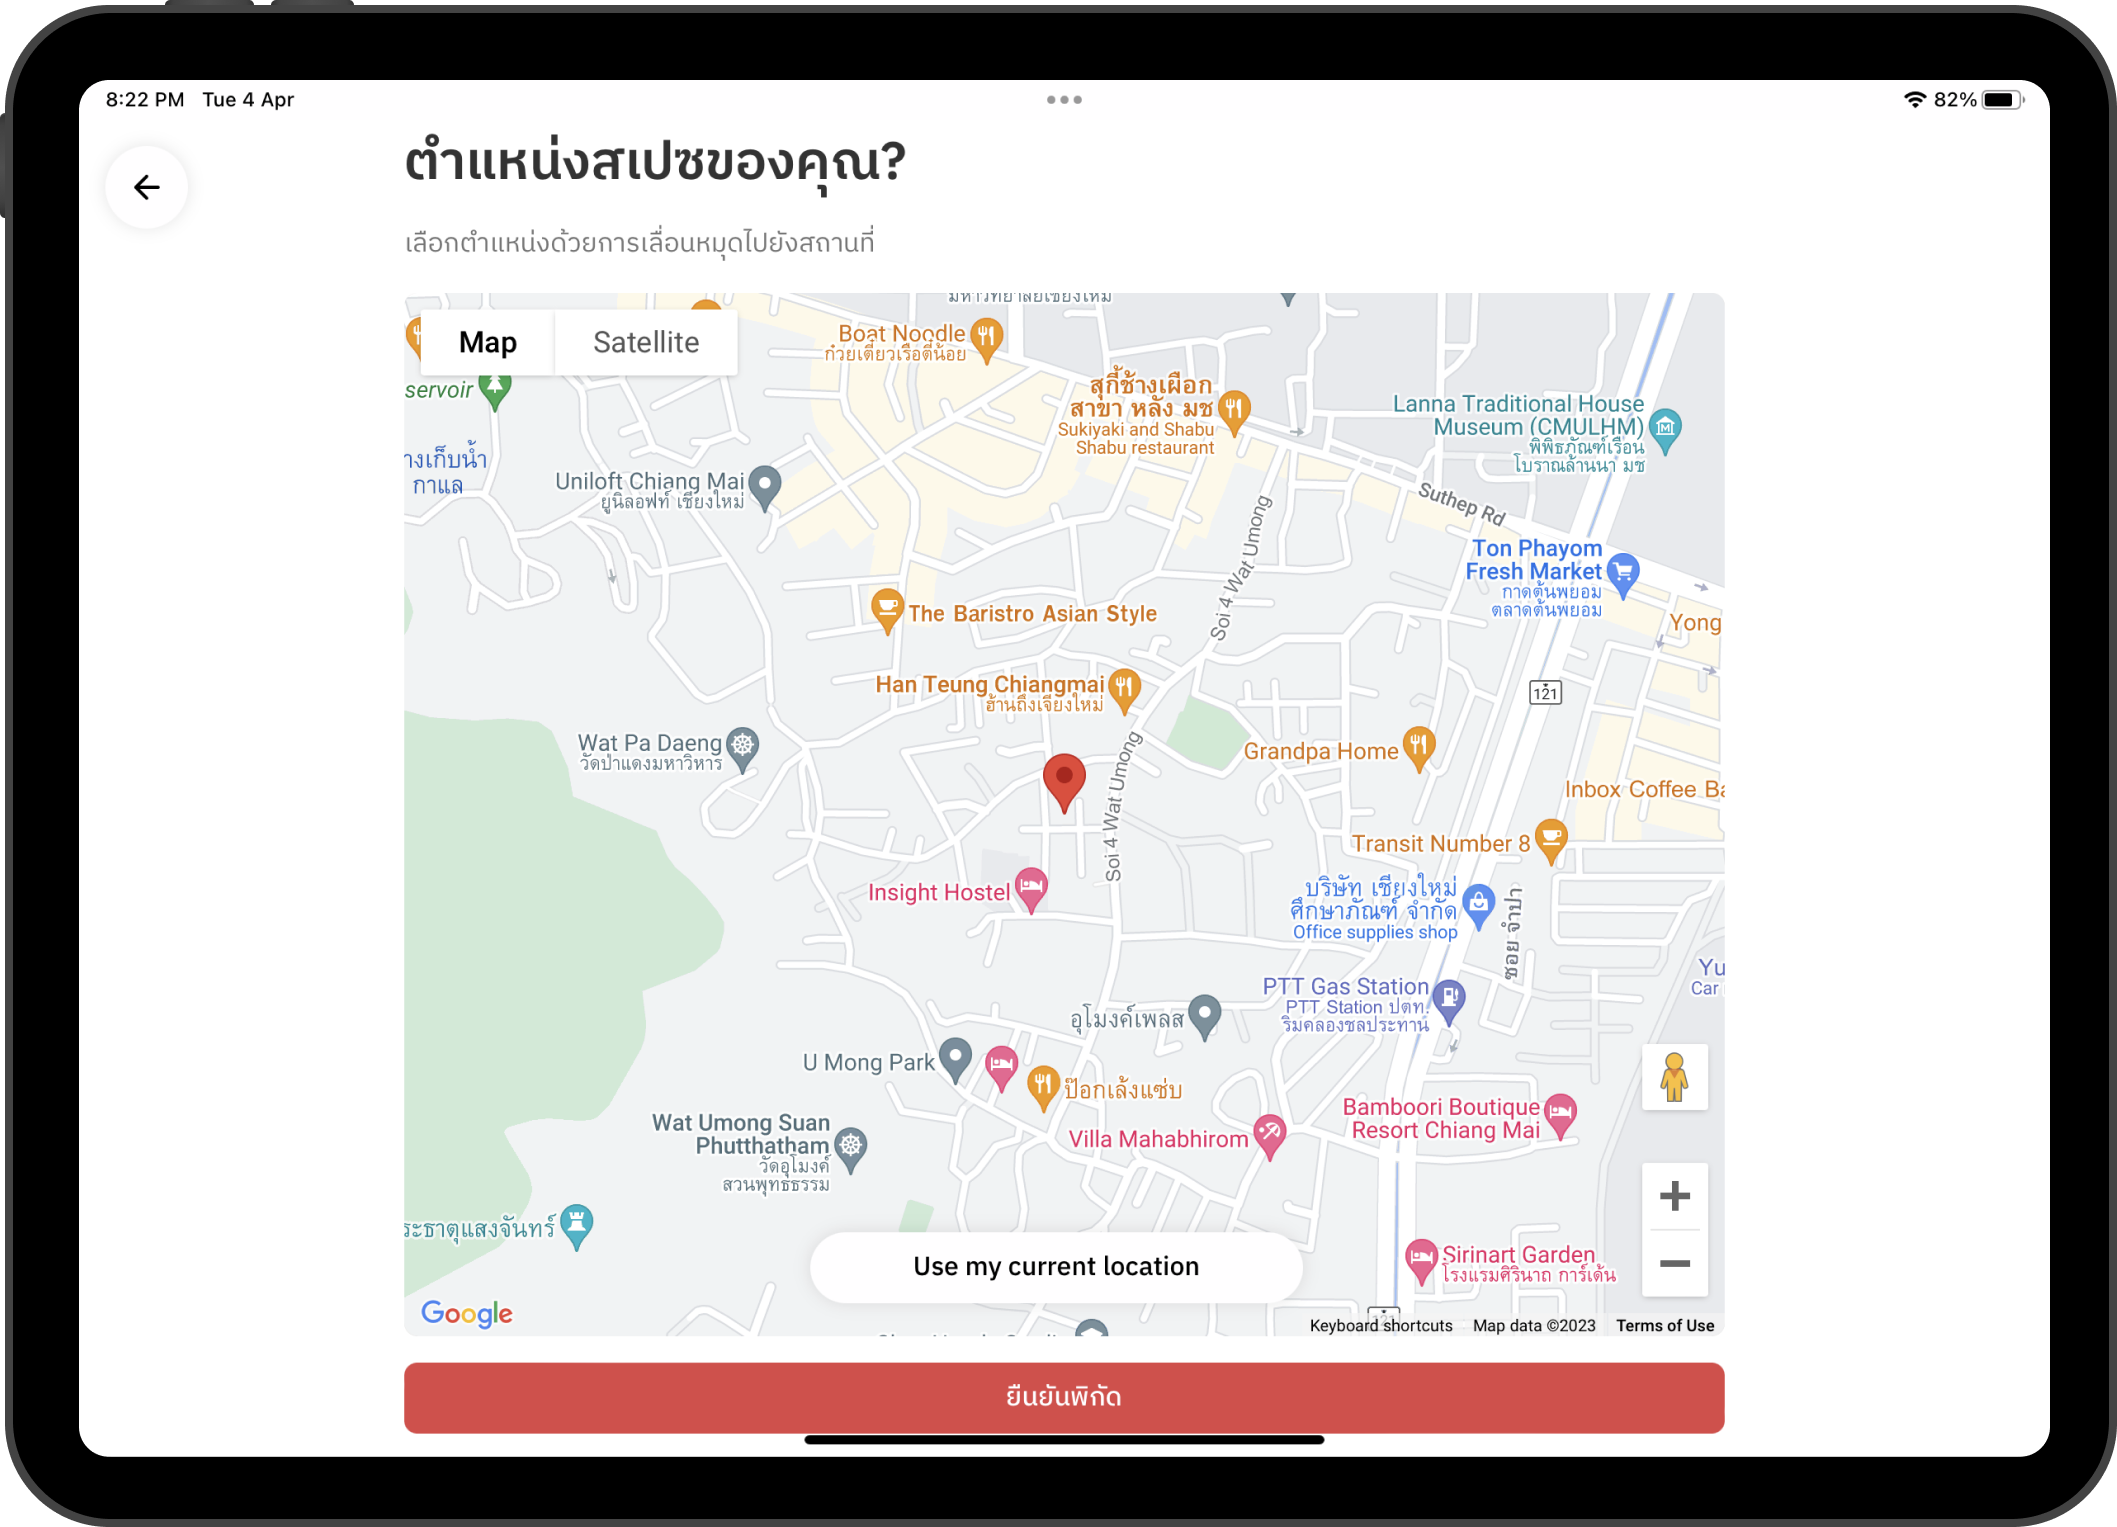
\includegraphics[width=5.5in]{./image/Flowider_place_location.png}
    \end{center}
    \caption[Flowider place location]{หน้าระบุตำแหน่งของสเปซ}
    \label{fig:Flowider_place_location}
\end{figure}
\begin{figure}[ht]
    \begin{center}
    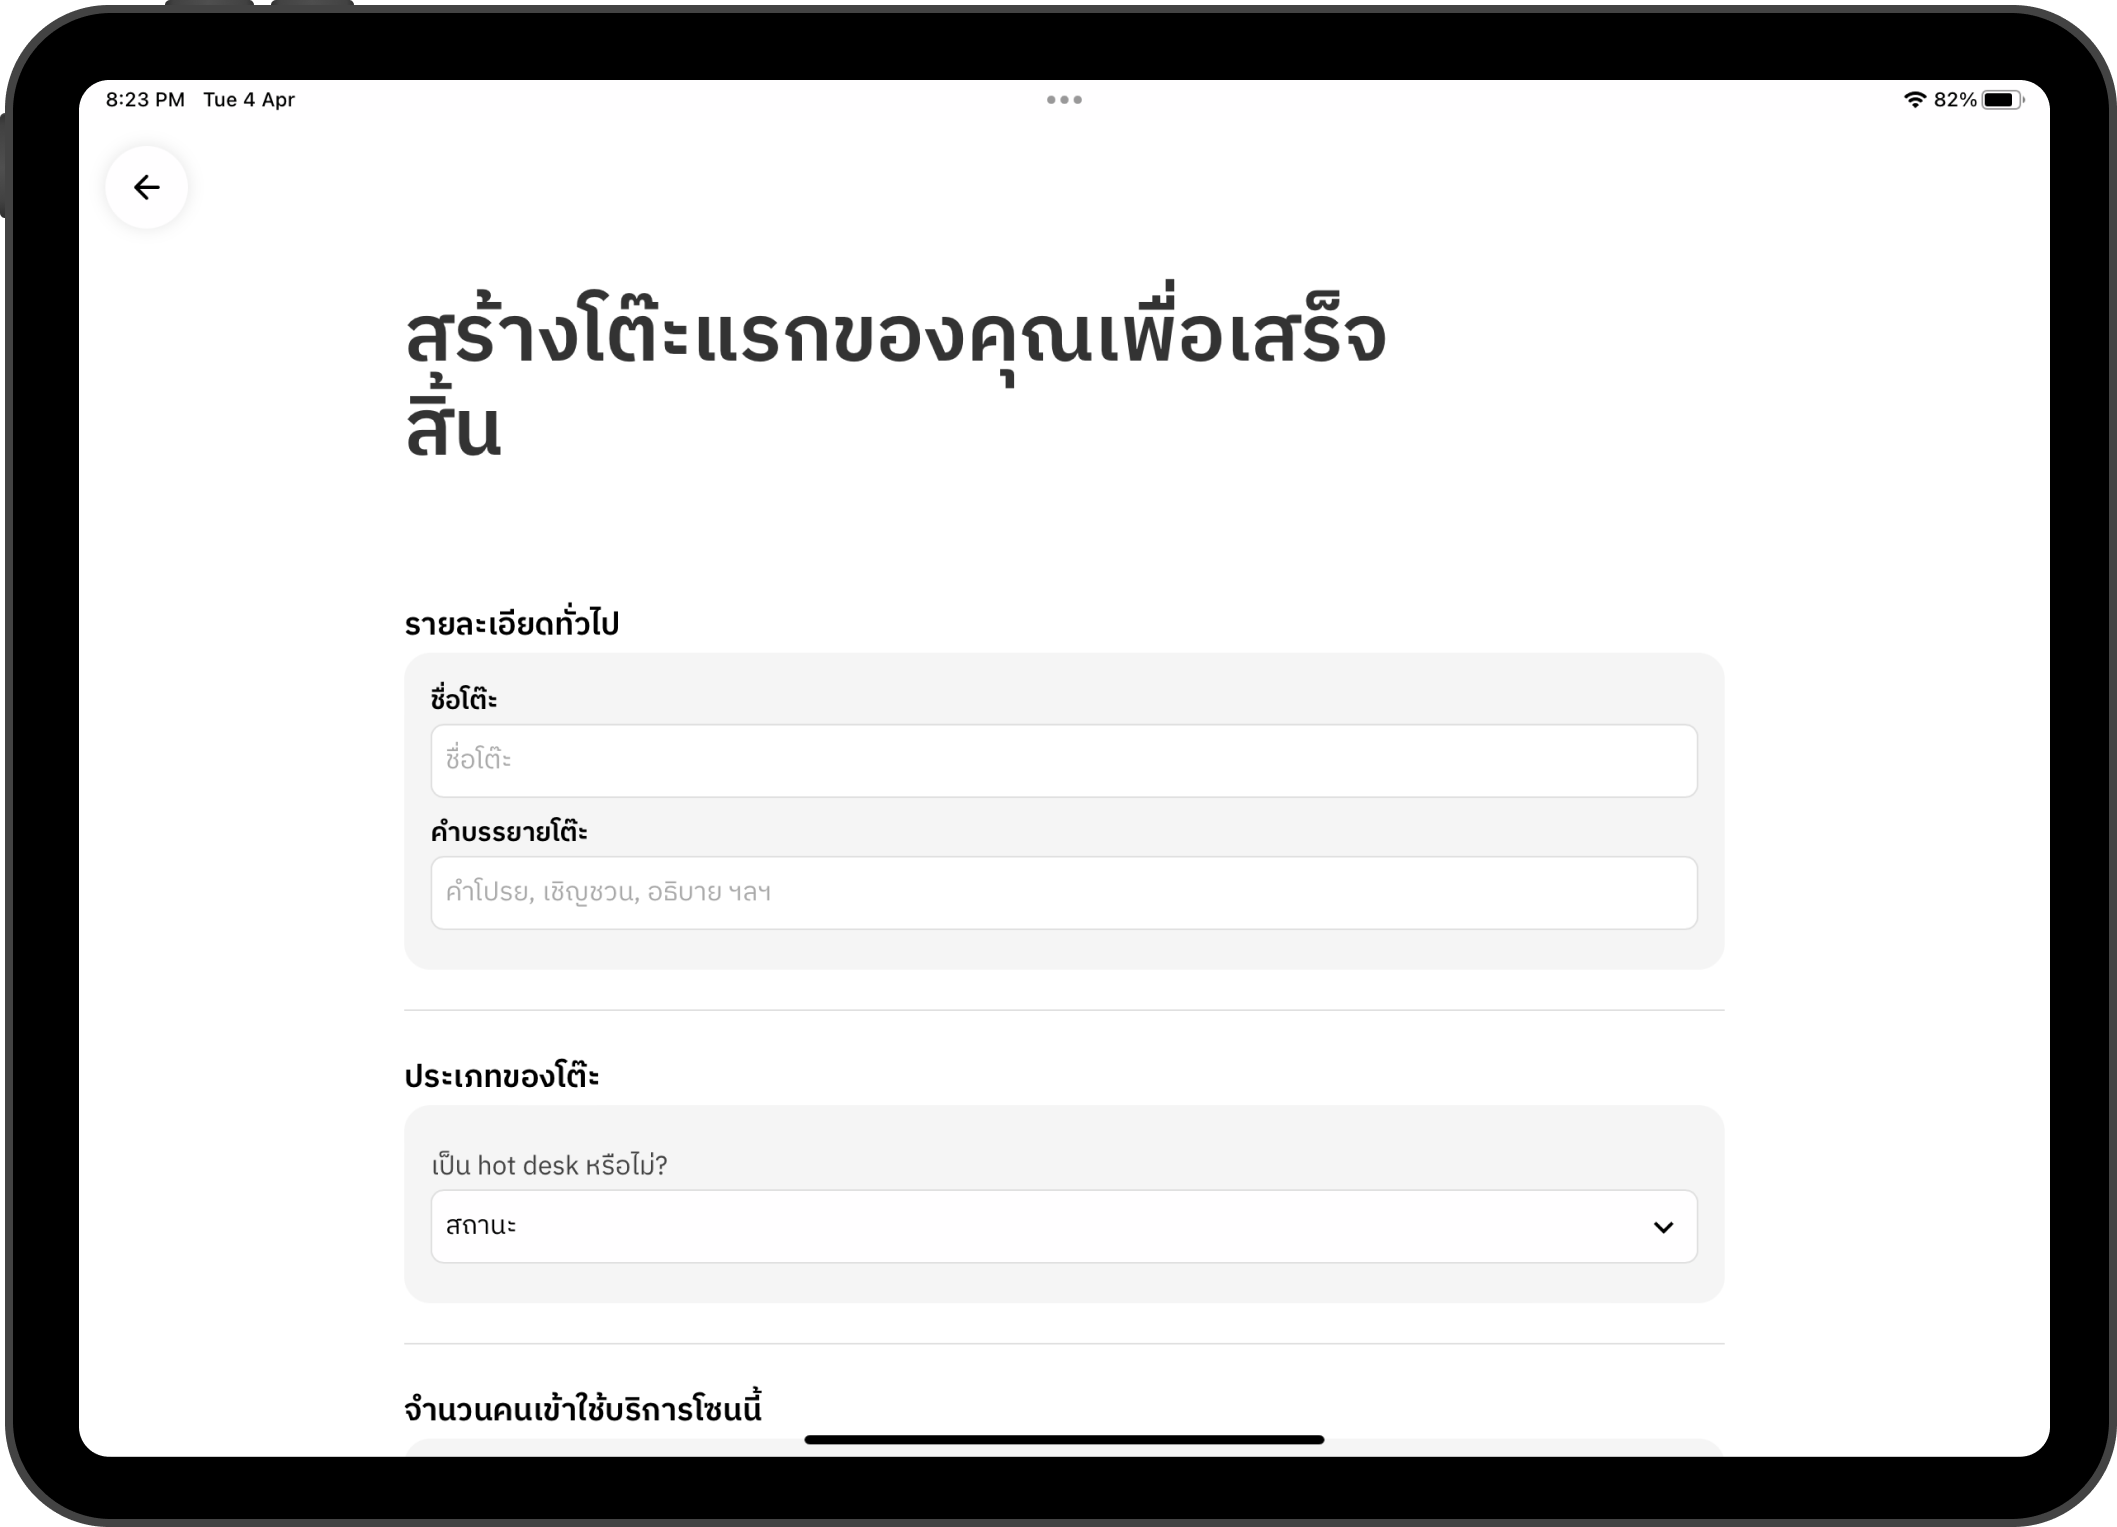
\includegraphics[width=5.5in]{./image/Flowider_desk_1.png}
    \end{center}
    \caption[Flowider desk 1]{หน้าระบุรายระเอียดของโต๊ะ}
    \label{fig:Flowider_desk_1}
\end{figure}
\begin{figure}[ht]
    \begin{center}
    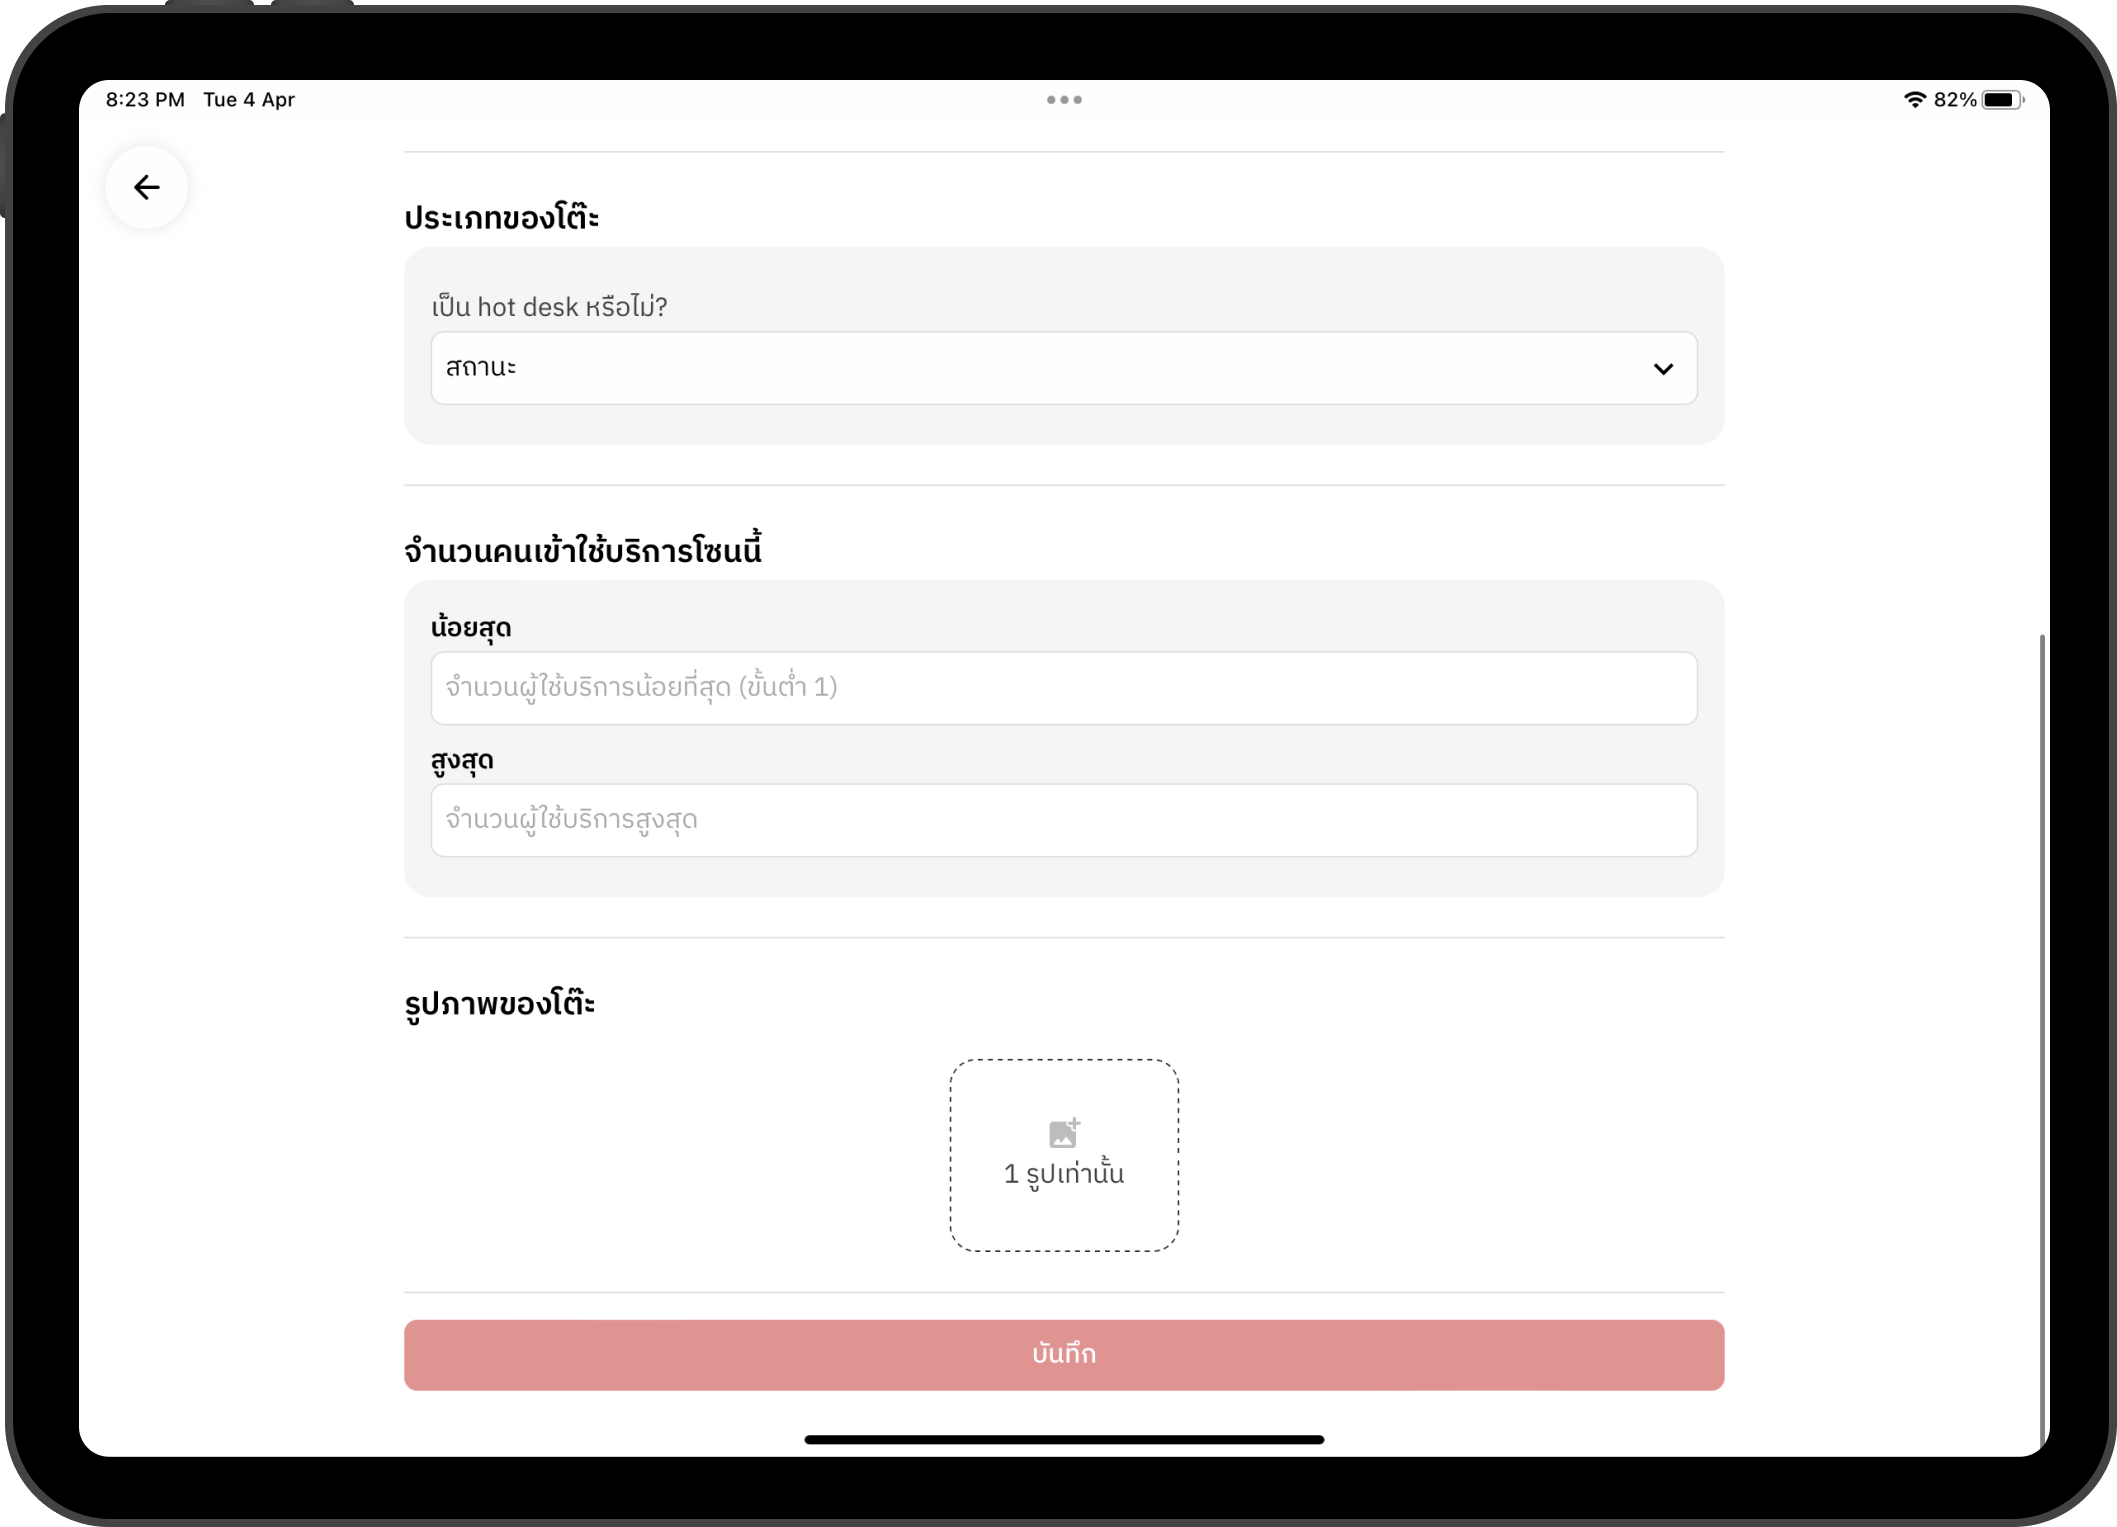
\includegraphics[width=5.5in]{./image/Flowider_desk_2.png}
    \end{center}
    \caption[Flowider desk 2]{หน้าระบุรายระเอียดของโต๊ะ (ต่อ)}
    \label{fig:Flowider_desk_2}
\end{figure}
